% Seminar report -- KTU B.Tech seminar report format
% Build: latexmk -pdf main.tex   (see README.md)
\pdfminorversion=7
\documentclass[12pt,a4paper,oneside]{report}

% ---------------------------------------------------------------- details
% Edit these if any of the names below need to change.
\newcommand{\reporttitle}{Beyond Pure Transformers: A Study of Hybrid Mamba-Transformer Architectures in NVIDIA's Nemotron~3 Super}
\newcommand{\studentname}{Rohith Chandran}
\newcommand{\registerno}{LKNP23AD042}
\newcommand{\programme}{Artificial Intelligence and Data Science}
\newcommand{\department}{Computer Science and Engineering}
\newcommand{\deptshort}{CSE}
\newcommand{\college}{College of Engineering Karunagappally}
\newcommand{\collegeplace}{Karunagappally, Kollam, Kerala}
\newcommand{\university}{APJ Abdul Kalam Technological University}
\newcommand{\reportmonth}{October 2026}
% Not given in the inputs -- fill these in before printing.
\newcommand{\guidename}{[Name of Seminar Guide]}
\newcommand{\guidedesignation}{[Designation]}
\newcommand{\coordinatorname}{[Name of Seminar Coordinator]}
\newcommand{\coordinatordesignation}{[Designation]}
\newcommand{\hodname}{[Name of Head of Department]}
\newcommand{\principalname}{[Name of Principal]}

% ---------------------------------------------------------------- packages
\usepackage[T1]{fontenc}
\usepackage[utf8]{inputenc}
\usepackage{mathptmx}
\usepackage{amsmath,amssymb}
\usepackage[a4paper,left=1.25in,right=1in,top=1in,bottom=1in,footskip=0.5in]{geometry}
\usepackage{setspace}
\usepackage{graphicx}
\usepackage{xcolor}
\usepackage{booktabs}
\usepackage{tabularx}
\usepackage{multirow}
\usepackage{array}
\usepackage{float}
\usepackage{enumitem}
\usepackage[font=small,labelfont=bf,labelsep=colon,skip=8pt]{caption}
\usepackage{subcaption}
\usepackage{titlesec}
\usepackage{fancyhdr}
\usepackage{microtype}
\usepackage{tikz}
\usepackage{pgfplots}
\pgfplotsset{compat=1.18}
\usetikzlibrary{arrows.meta,positioning,calc,fit,shapes.geometric}
\usepackage{xurl}
\usepackage[hidelinks,pdfusetitle,bookmarksnumbered]{hyperref}

\graphicspath{{figures/}}
\hypersetup{
  pdftitle={Beyond Pure Transformers: A Study of Hybrid Mamba-Transformer Architectures in NVIDIA's Nemotron 3 Super},
  pdfauthor={\studentname},
  pdfsubject={B.Tech Seminar Report}
}

% ---------------------------------------------------------------- layout
\onehalfspacing
\setlength{\parindent}{1.25cm}
\setlength{\emergencystretch}{2em}
\setlist{itemsep=2pt,topsep=4pt,parsep=2pt}
\renewcommand{\arraystretch}{1.2}
\newcolumntype{L}{>{\raggedright\arraybackslash}X}
\newcolumntype{P}[1]{>{\raggedright\arraybackslash}p{#1}}

\titleformat{\chapter}[display]
  {\normalfont\Large\bfseries\centering}
  {\MakeUppercase{\chaptertitlename}~\thechapter}{6pt}{\MakeUppercase}
\titleformat{name=\chapter,numberless}[block]
  {\normalfont\Large\bfseries\centering}{}{0pt}{\MakeUppercase}
\titlespacing*{\chapter}{0pt}{-10pt}{24pt}
\titleformat{\section}{\normalfont\large\bfseries}{\thesection}{0.8em}{}
\titleformat{\subsection}{\normalfont\normalsize\bfseries}{\thesubsection}{0.8em}{}
\titlespacing*{\section}{0pt}{14pt}{6pt}
\titlespacing*{\subsection}{0pt}{10pt}{4pt}

\newcommand{\footerdept}{Department of \deptshort, \college}
\fancypagestyle{mainmatter}{%
  \fancyhf{}%
  \fancyfoot[L]{\small\footerdept}%
  \fancyfoot[R]{\small\thepage}%
  \renewcommand{\headrulewidth}{0pt}%
  \renewcommand{\footrulewidth}{0.4pt}}
\fancypagestyle{frontmatter}{%
  \fancyhf{}%
  \fancyfoot[C]{\small\thepage}%
  \renewcommand{\headrulewidth}{0pt}%
  \renewcommand{\footrulewidth}{0pt}}

% Source line for figures taken from the literature
\newcommand{\source}[1]{\emph{Source:} #1.}
% Model names used throughout
\newcommand{\NS}{Nemotron~3 Super}
\newcommand{\NN}{Nemotron~3 Nano}

\begin{document}
\makeatletter
\def\bstctlcite#1{\@bsphack\@for\@citeb:=#1\do{\edef\@citeb{\expandafter\@firstofone\@citeb}\if@filesw\immediate\write\@auxout{\string\citation{\@citeb}}\fi}\@esphack}
\makeatother
\bstctlcite{bstctl}

% ================================================================ front matter
\pagenumbering{roman}
\pagestyle{frontmatter}
\fancypagestyle{plain}{%
  \fancyhf{}\fancyfoot[C]{\small\thepage}%
  \renewcommand{\headrulewidth}{0pt}\renewcommand{\footrulewidth}{0pt}}

\thispagestyle{empty}
\begin{center}
\singlespacing
\vspace*{0.3cm}
{\LARGE\bfseries Beyond Pure Transformers: A Study of Hybrid Mamba-Transformer Architectures in NVIDIA's Nemotron~3 Super\par}
\vspace{1.6cm}
{\large\itshape A Seminar Report\par}
\vspace{0.5cm}
{\normalsize\itshape Submitted to the \university\par}
\vspace{0.2cm}
{\normalsize\itshape in partial fulfillment of requirements for the award of degree\par}
\vspace{0.5cm}
{\large\bfseries\itshape Bachelor of Technology\par}
\vspace{0.3cm}
{\itshape in\par}
\vspace{0.3cm}
{\large\bfseries\itshape \programme\par}
\vspace{0.3cm}
{\itshape by\par}
\vspace{0.4cm}
{\large\bfseries\MakeUppercase{\studentname}\par}
\vspace{0.2cm}
{\large\bfseries \registerno\par}
\vspace{1.0cm}

\includegraphics[width=4.6cm]{logo.png}\par
\vspace{1.2cm}
{\bfseries\small\MakeUppercase{Department of \department}\par}
\vspace{0.1cm}
{\bfseries\small\MakeUppercase{\college}\par}
\vspace{0.1cm}
{\bfseries\small KERALA\par}
\vspace{0.1cm}
{\bfseries\footnotesize \reportmonth\par}
\end{center}
\clearpage

\thispagestyle{empty}
\begin{center}
\singlespacing
{\bfseries DEPT. OF \MakeUppercase{\department}\\ \MakeUppercase{\college}\par}
\vspace{0.3cm}
{\bfseries \acyear\par}
\vspace{0.5cm}

\includegraphics[width=3.4cm]{logo.png}\par
\vspace{0.8cm}
{\bfseries CERTIFICATE\par}
\end{center}
\vspace{0.3cm}
\begingroup
\doublespacing\hyphenpenalty=10000\exhyphenpenalty=10000
\noindent\hspace{1.2em}This is to certify that the report entitled
\textbf{\reporttitle} submitted by \mbox{\textbf{\MakeUppercase{\studentname}}}
\mbox{(\registerno)}, to the \university\ in partial fulfillment of the B.Tech.\
degree in \programme\ is a bonafide record of the seminar work carried out by
him under our guidance and supervision. This report in any form has not been
submitted to any other University or Institute for any purpose.
\par\endgroup
\vspace{1.2cm}

\begingroup\singlespacing
% Guide at the left margin, coordinator at the right margin, HOD centred below
\noindent
\begin{tabular}[t]{@{}l@{}}
\textbf{\guidename}\\ (Seminar Guide)\\ \guidedesignation\\ Dept.\ of \deptshort\\ College of Engineering\\ Karunagappally
\end{tabular}\hfill
\begin{tabular}[t]{@{}l@{}}
\textbf{\coordinatorname}\\ (Seminar Coordinator)\\ \coordinatordesignation\\ Dept.\ of \deptshort\\ College of Engineering\\ Karunagappally
\end{tabular}

\vspace{1.0cm}
\begin{center}
\begin{tabular}{@{}c@{}}
\textbf{\hodname}\\ Associate Professor and HOD\\ Dept.\ of \deptshort\\ College of Engineering\\ Karunagappally
\end{tabular}
\end{center}
\endgroup
\clearpage

\chapter*{Declaration}
\addcontentsline{toc}{chapter}{Declaration}

I, the undersigned, hereby declare that the seminar report entitled
\textbf{``\reporttitle''}, submitted in partial fulfilment of the requirements
for the award of the degree of Bachelor of Technology of the \university,
Kerala, is a bonafide work done by me under the supervision of \guidename. This
submission represents my ideas in my own words, and where ideas or words of
others have been included, I have adequately and accurately cited and
referenced the original sources. Figures reproduced from published papers are
identified as such in their captions together with the source.

I also declare that I have adhered to the ethics of academic honesty and
integrity and have not misrepresented or fabricated any data, idea, fact or
source in this submission. I understand that any violation of the above will be
a cause for disciplinary action by the institute and/or the University and can
also evoke penal action from the sources which have not been properly cited or
from whom proper permission has not been obtained. This report has not
previously formed the basis for the award of any degree, diploma or similar
title of any other university.

\vspace{2.2cm}
\noindent
\begin{minipage}[t]{0.48\linewidth}
\raggedright\singlespacing
Place: Karunagappally\\[4pt]
Date:
\end{minipage}\hfill
\begin{minipage}[t]{0.48\linewidth}
\raggedleft\singlespacing
\textbf{\studentname}\\
\registerno
\end{minipage}

\chapter*{Acknowledgement}
\addcontentsline{toc}{chapter}{Acknowledgement}

I take this opportunity to express my deepest sense of gratitude and sincere
thanks to everyone who helped me to complete this work successfully. I am
profoundly grateful to \principalname, The Principal, \college\ for her
encouragement, constant support, and for providing the necessary facilities
that enabled me to carry out this seminar work successfully.

I express my sincere thanks to \hodname, Head of Department, \department,
\college\ for providing me with all the necessary facilities and support.

I would like to express my sincere gratitude to \coordinatorname,
\coordinatordesignation, \department, \college\ for their support and
co-operation.

I would like to place on record my sincere gratitude to my seminar guide
\guidename, \guidedesignation, \department, \college\ for the guidance and
mentorship throughout the course.

Finally I thank my family, and friends who contributed to the successful
fulfilment of this seminar work.

\vspace{0.8cm}
\noindent\textbf{\MakeUppercase{\studentname}}\\
Department of \deptshort, \college

\chapter*{Abstract}
\addcontentsline{toc}{chapter}{Abstract}

Since 2017, the Transformer architecture has been the standard foundation for
large language models. However, its self-attention mechanism compares every
token with every other token and must keep a key--value cache that grows with
the input, so it becomes computationally expensive and memory-hungry as the
context length increases. This seminar studies Nemotron~3 Super, an open
language model released by NVIDIA in April 2026, which replaces most attention
layers with Mamba-2 state-space layers, keeps a small number of attention
layers as global ``anchors'', and scales its capacity with a Mixture-of-Experts
(MoE) design. The model has 120~billion parameters in total, of which only
about 12~billion are active for each token, and it supports context windows of
up to one million tokens.

The report first explains why pure Transformers struggle on long inputs and how
selective state-space models such as Mamba and Mamba-2 keep a constant-size
state instead. It then describes the three architectural ideas that distinguish
Nemotron~3 Super: the interleaved hybrid Mamba--attention layout of its 88
layers, LatentMoE, which runs 512 experts in a compressed 1024-dimensional
latent space, and shared-weight Multi-Token Prediction heads that enable native
speculative decoding. The training pipeline is examined next, covering 4-bit
NVFP4 pretraining on 25~trillion tokens, long-context extension, supervised
fine-tuning and multi-environment reinforcement learning, followed by
post-training quantization and the stochastic-rounding fix required for the
Mamba state cache.

On published benchmarks the model reaches accuracy comparable to
GPT-OSS-120B and Qwen3.5-122B while delivering up to 2.2$\times$ and
7.5$\times$ higher inference throughput than these two models respectively, and
it retains a RULER score of 91.6 at a one-million-token context. The report
closes with the applications, advantages and limitations of the design and
argues that hybrid architectures are a significant step beyond
Transformer-only models for efficient, large-scale AI systems.

\vspace{0.6cm}
\noindent\textbf{Keywords:} large language models, state-space models, Mamba-2,
hybrid architecture, Mixture-of-Experts, LatentMoE, multi-token prediction,
NVFP4, quantization, long-context inference.

\vspace{0.8cm}
\noindent\textbf{\MakeUppercase{\studentname}}\\
\registerno


\begingroup
\singlespacing
\tableofcontents
\clearpage
\phantomsection\addcontentsline{toc}{chapter}{List of Figures}
\listoffigures
\clearpage
\phantomsection\addcontentsline{toc}{chapter}{List of Tables}
\listoftables
\endgroup
\chapter*{List of Abbreviations}
\addcontentsline{toc}{chapter}{List of Abbreviations}

\begingroup
\singlespacing
\renewcommand{\arraystretch}{1.25}
\noindent
\begin{tabularx}{\linewidth}{@{}P{2.6cm}L@{}}
AI      & Artificial Intelligence \\
API     & Application Programming Interface \\
BF16    & 16-bit ``brain'' floating-point format (bfloat16) \\
CPT     & Continuous Pretraining \\
FFN     & Feed-Forward Network \\
FLOP    & Floating-Point Operation \\
FP4/FP8 & 4-bit / 8-bit floating-point formats \\
GEMM    & General Matrix--Matrix Multiplication \\
GenRM   & Generative Reward Model \\
GPU     & Graphics Processing Unit \\
GQA     & Grouped-Query Attention \\
GRPO    & Group Relative Policy Optimization \\
KV      & Key--Value (cache) \\
LLM     & Large Language Model \\
LR      & Learning Rate \\
MoE     & Mixture-of-Experts \\
MSE     & Mean Squared Error \\
MTP     & Multi-Token Prediction \\
MXFP4/8 & Microscaling 4-bit / 8-bit floating-point formats \\
NVFP4   & NVIDIA 4-bit block-scaled floating-point format \\
PTQ     & Post-Training Quantization \\
QAD/QAT & Quantization-Aware Distillation / Training \\
RHT     & Random Hadamard Transform \\
RL      & Reinforcement Learning \\
RLHF    & Reinforcement Learning from Human Feedback \\
RLVR    & Reinforcement Learning from Verifiable Rewards \\
RTNE    & Round To Nearest, ties to Even \\
SFT     & Supervised Fine-Tuning \\
SR      & Stochastic Rounding \\
SSD     & Structured State Space Duality \\
SSM     & State Space Model \\
SWE     & Software Engineering \\
TPS     & Tokens Per Second \\
WSD     & Warmup--Stable--Decay (learning-rate schedule) \\
\end{tabularx}
\endgroup


% ================================================================ main matter
\clearpage
\pagenumbering{arabic}
\pagestyle{mainmatter}
\fancypagestyle{plain}{%
  \fancyhf{}\fancyfoot[L]{\small\footerdept}\fancyfoot[R]{\small\thepage}%
  \renewcommand{\headrulewidth}{0pt}\renewcommand{\footrulewidth}{0.4pt}}

\chapter{Introduction}
\label{ch:intro}

\section{Background}

Almost every large language model (LLM) in use today is built on the
Transformer architecture introduced by Vaswani et al.\ in
2017~\cite{vaswani2017attention}. Its central operation, self-attention, lets
every token in the input look directly at every other token, which gives the
model an exceptionally flexible way of routing information across a sequence.
That flexibility has a price. The amount of computation in an attention layer
grows quadratically with the length of the input, and during text generation
the model must keep the keys and values of all previous tokens in a
\emph{key--value (KV) cache} whose size grows with every token that is added.
For a chat message of a few hundred tokens this cost is negligible. For the
workloads that are now becoming common---an AI agent that reads an entire code
repository, works through a long tool-calling session, or analyses a
several-hundred-page document---it becomes the dominant cost of running the
model.

Two independent lines of research have attacked this cost from different
directions. The first is the \emph{state-space model} (SSM). Mamba~\cite{gu2023mamba}
and its successor Mamba-2~\cite{dao2024mamba2} read a sequence one token at a
time and summarise everything seen so far in a state of fixed size, so that
time grows only linearly with the sequence length and the memory needed during
generation does not grow at all. The second is the \emph{Mixture-of-Experts}
(MoE) layer~\cite{shazeer2017moe,lepikhin2020gshard}, which splits the
feed-forward part of a model into many small ``experts'' and activates only a
handful of them for each token, so that a model can hold a very large number of
parameters while spending the computation of a much smaller one.

\NS, released by NVIDIA in April 2026~\cite{nvidia2026super}, combines both
ideas in a single open model. It has 120.6~billion parameters in total, of
which only 12.7~billion are active in any forward pass. Most of its 88 layers
are Mamba-2 and MoE layers; only eight are self-attention layers. The model
accepts contexts of up to one million tokens and, according to its technical
report, achieves accuracy comparable to GPT-OSS-120B~\cite{openai2025gptoss}
and Qwen3.5-122B while delivering up to 2.2$\times$ and 7.5$\times$ higher
inference throughput than those models respectively.

\section{Motivation}

The motivation for studying this model is that it is the clearest example so
far of a production-scale LLM that is \emph{not} a pure Transformer. Earlier
hybrid models were either small or research prototypes. \NS\ shows that the
hybrid approach scales to more than one hundred billion parameters and to
million-token contexts while remaining competitive with the strongest open
Transformer models of the same size. Understanding how it works therefore
answers a broader question: is the attention-only design that has dominated
since 2017 still the best foundation for large models, or is the field moving
towards mixed architectures in which attention is used sparingly?

A second motivation is that the model is fully open. Its weights, a large part
of its training data and its training recipe are published, and the technical
report describes the engineering in unusual detail---including problems that
appeared along the way, such as the numerical drift caused by quantizing the
Mamba state. This makes it possible to study not only the architecture but
also what it takes to train and deploy it.

\section{Objectives of the Seminar}

The objectives of this seminar are:
\begin{itemize}
  \item to understand why Transformers become slow and memory-heavy on long
        inputs;
  \item to explore state-space models, in particular Mamba and Mamba-2, which
        were proposed to solve that problem;
  \item to study how \NS\ interleaves Mamba-2 and attention layers to form a
        hybrid model;
  \item to examine how Mixture-of-Experts, and specifically LatentMoE, lets the
        model stay large while running cheaply;
  \item to review how the model is trained, quantized and evaluated; and
  \item to highlight what this design suggests about the future of efficient
        large-scale AI.
\end{itemize}

\section{Scope}

The report is a study of published work. Its primary source is the \NS\
technical report~\cite{nvidia2026super}; the supporting papers on Mamba,
Mamba-2, LatentMoE, multi-token prediction and NVFP4 training are used to
explain the building blocks in more depth. All benchmark numbers quoted in this
report are those published by the respective authors; no new experiments were
run. Where the report contains estimates worked out by the author from
published configuration values, this is stated explicitly.

\section{Organisation of the Report}

Chapter~\ref{ch:survey} surveys the literature that leads up to \NS.
Chapter~\ref{ch:background} gives the technical background on Transformers and
the KV cache, state-space models, and Mixture-of-Experts.
Chapter~\ref{ch:arch} describes the architecture of \NS: the hybrid layout,
LatentMoE and multi-token prediction. Chapter~\ref{ch:training} covers
pretraining in the 4-bit NVFP4 format, the training data, long-context
extension, supervised fine-tuning and reinforcement learning.
Chapter~\ref{ch:quant} explains how the model is quantized for deployment and
how the Mamba state is handled. Chapter~\ref{ch:results} presents the results,
Chapter~\ref{ch:apps} the applications, and
Chapter~\ref{ch:adv} the advantages and limitations.
Chapter~\ref{ch:conclusion} concludes the report and outlines future scope.

\chapter{Literature Survey}
\label{ch:survey}

\NS\ brings together several existing ideas at a larger scale than before.
This chapter traces them through the literature.

\section{Transformers and State-Space Models}

The Transformer~\cite{vaswani2017attention} relates all pairs of positions in
one step, which makes it highly parallel and good at long-range dependencies
but quadratic in cost. Grouped-Query Attention (GQA)~\cite{ainslie2023gqa}
shrinks the KV cache by letting several query heads share one key--value head,
but does not change how it scales.

The Structured State Space model S4~\cite{gu2021s4} showed that a discretised
linear state-space system can model very long sequences, but its dynamics were
the same for every input. Mamba~\cite{gu2023mamba} made the parameters
\emph{functions of the input}, so the model decides token by token what to
store and what to ignore (Figure~\ref{fig:mamba-selective}); it was the first
linear-time model to match Transformers of similar size on language modelling.
Mamba-2~\cite{dao2024mamba2} introduced the \emph{structured state space
duality} (SSD) framework, showing that SSMs and a form of attention are two
views of the same structured matrices, and made the core layer 2--8$\times$
faster. Its remaining weakness is inherent: the state is a compressed summary,
so exact details from far back can fade.

\begin{figure}[!htbp]
  \centering
  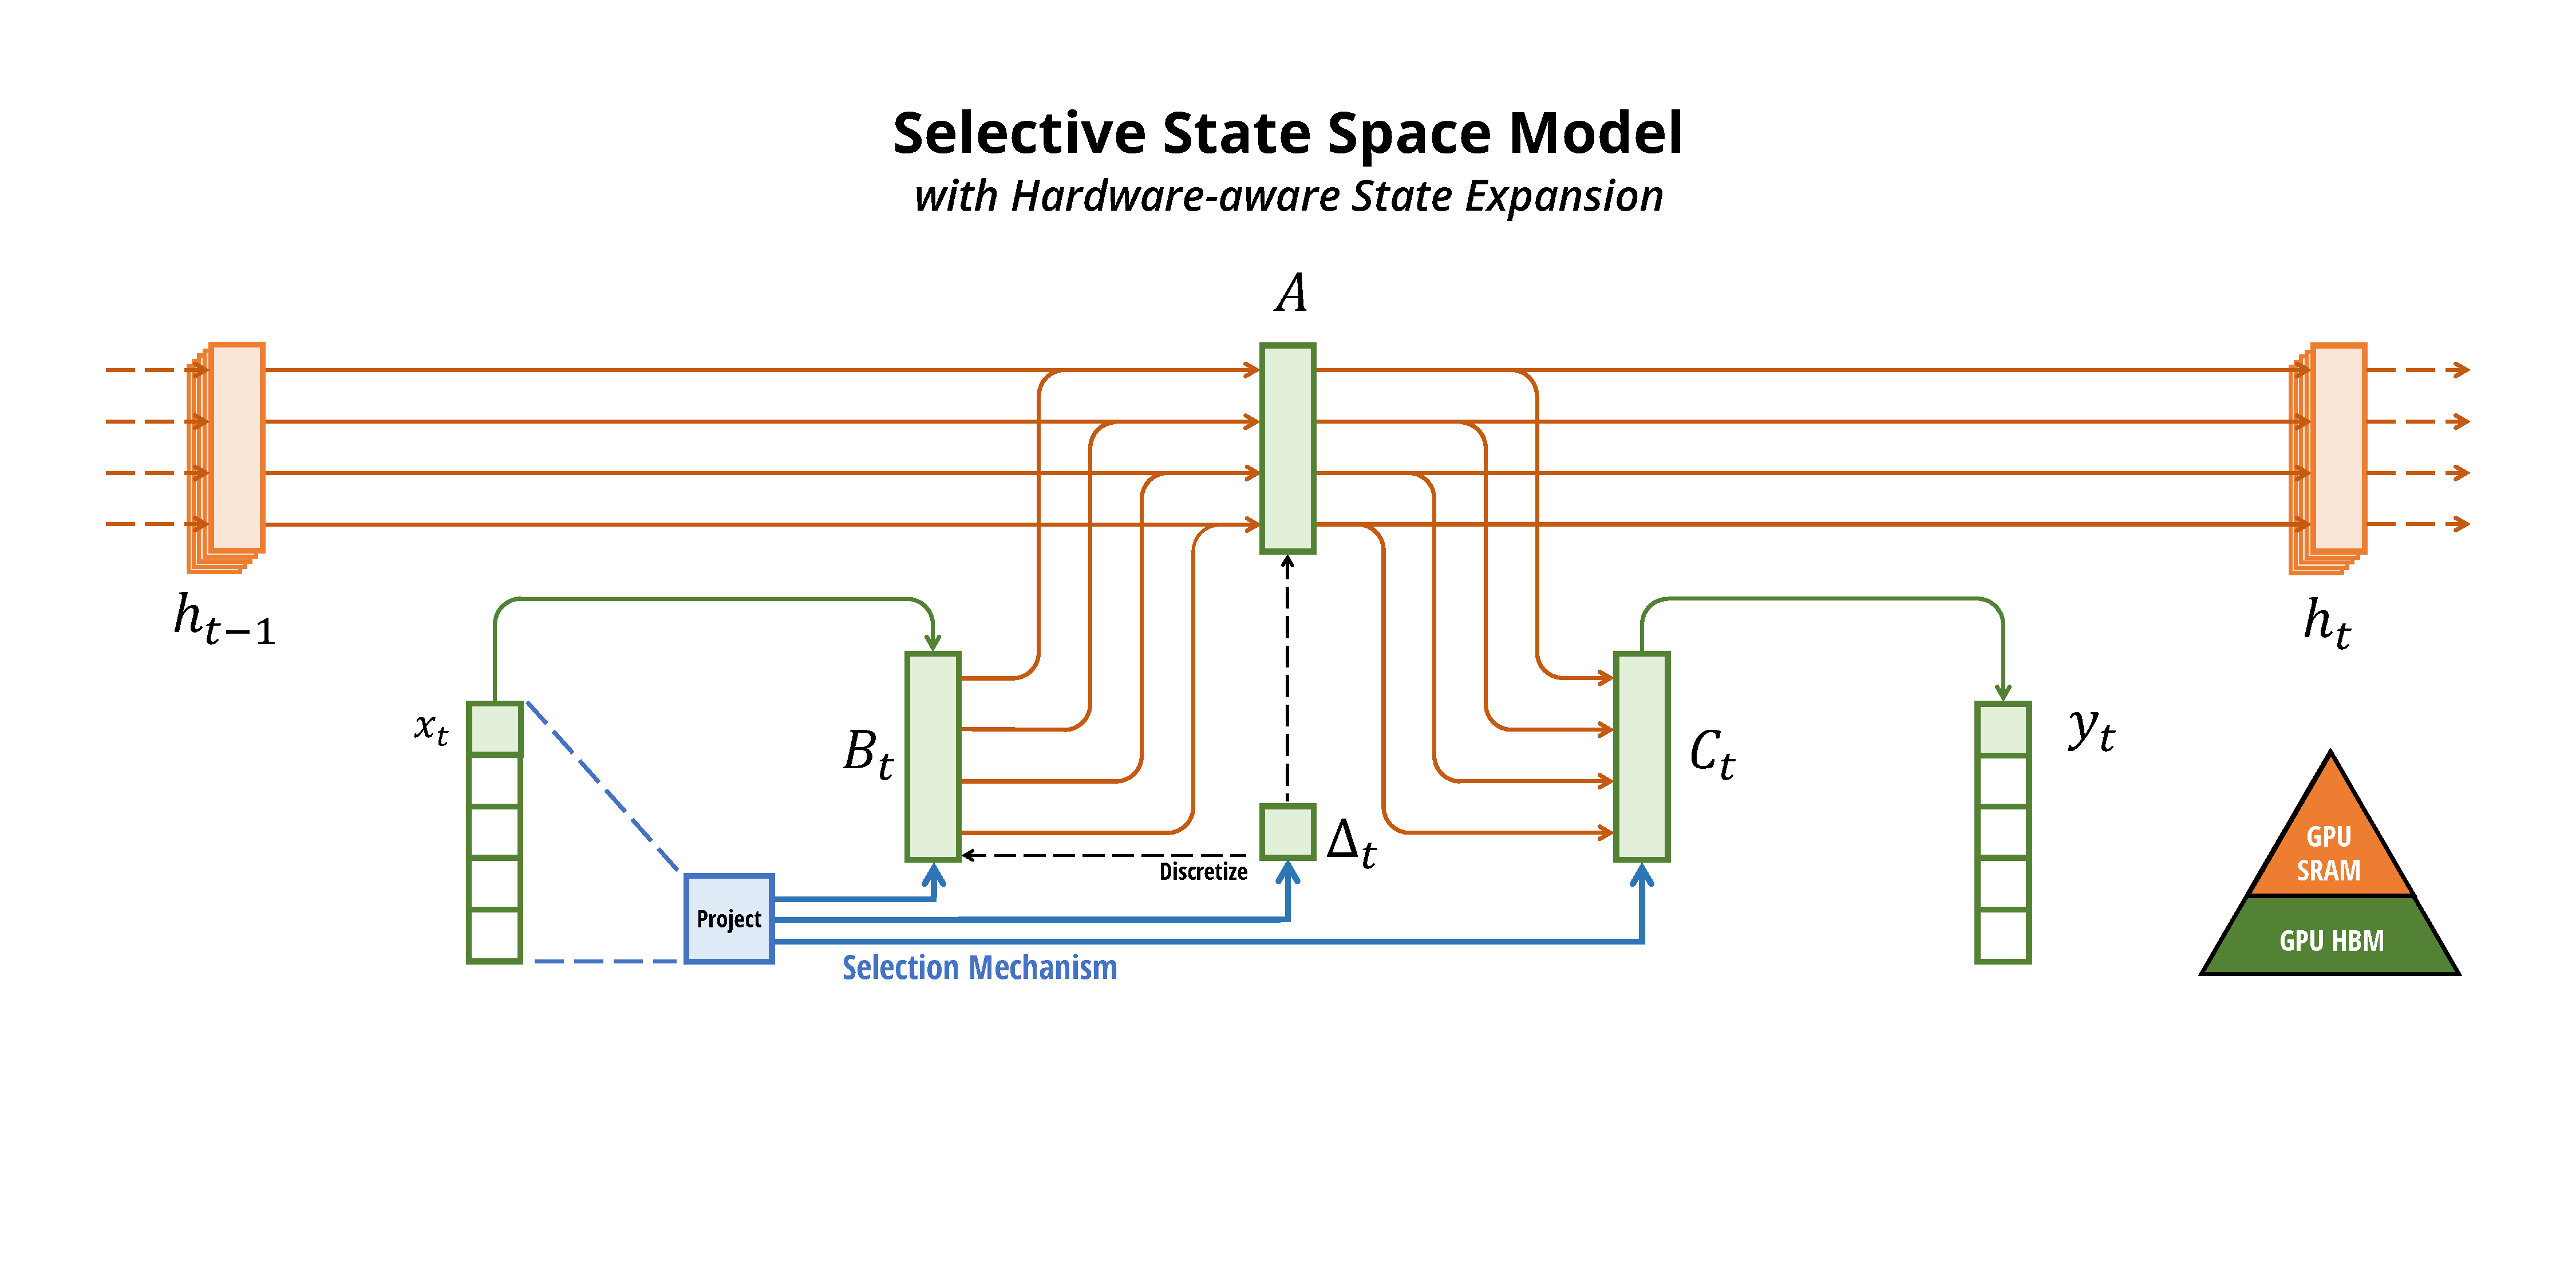
\includegraphics[width=0.9\linewidth]{mamba-fig01-selective-ssm.pdf}
  \caption[Selective state-space model with input-dependent parameters]{Selective
  state-space model: a selection mechanism makes the SSM parameters depend on
  the input. \source{Gu and Dao (2023)~\cite{gu2023mamba}, Fig.~1}}
  \label{fig:mamba-selective}
\end{figure}

\section{Hybrid Mamba--Transformer Models}

If Mamba is efficient but forgetful and attention is precise but expensive,
the natural step is to mix them. Jamba~\cite{lieber2024jamba} was the first
large model to interleave Transformer and Mamba layers with MoE
(Figure~\ref{fig:jamba}), supporting 256K-token contexts on a single 80\,GB
GPU.

\begin{figure}[!htbp]
  \centering
  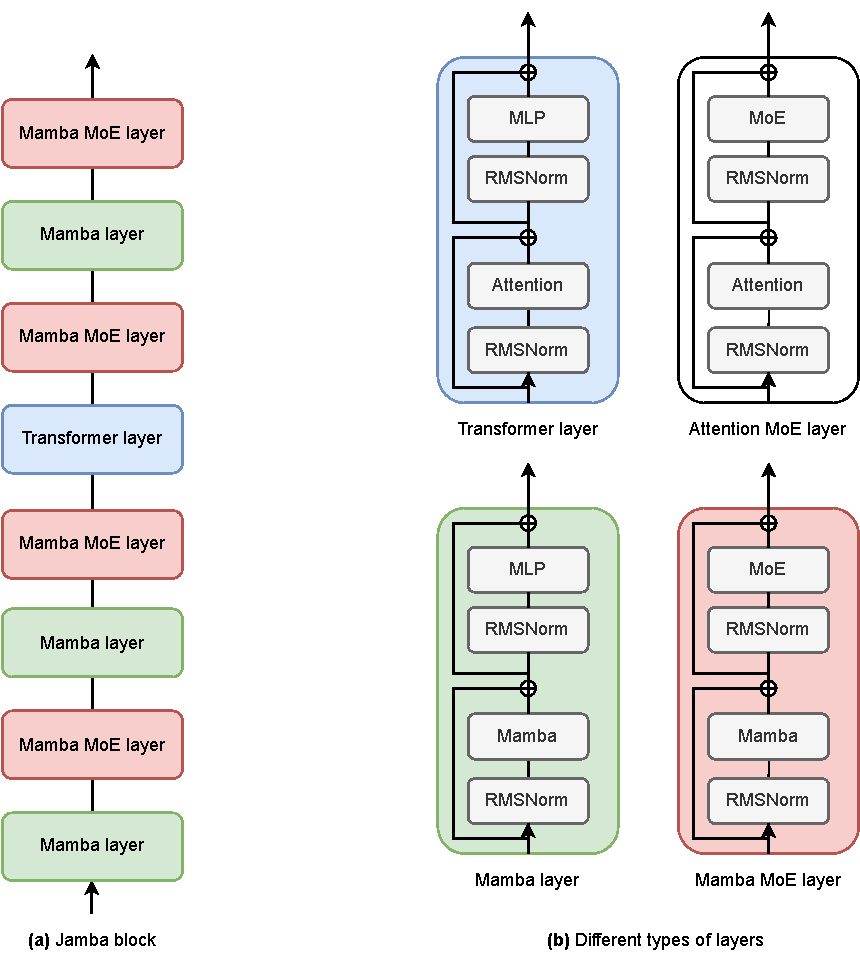
\includegraphics[width=0.5\linewidth]{jamba-fig01-block.pdf}
  \caption[A Jamba block mixing attention, Mamba and MoE layers]{(a) A Jamba
  block and (b) its layer types. \source{Lieber et al.\
  (2024)~\cite{lieber2024jamba}, Fig.~1}}
  \label{fig:jamba}
\end{figure}

Waleffe et al.~\cite{waleffe2024empirical} trained 8B Mamba, Mamba-2 and
Transformer models on the same data. Pure SSMs lagged on copying and
in-context learning tasks such as five-shot MMLU, but a hybrid of 43\%
Mamba-2, 7\% attention and 50\% MLP layers beat the Transformer on all twelve
tasks evaluated and was predicted to be up to 8$\times$ faster at generation.
Validation loss was lowest with only about 8\% attention layers
(Figure~\ref{fig:attn-ratio}): \emph{a few attention layers are enough}.

\begin{figure}[!htbp]
  \centering
  \begin{subfigure}[b]{0.44\linewidth}
    \centering
    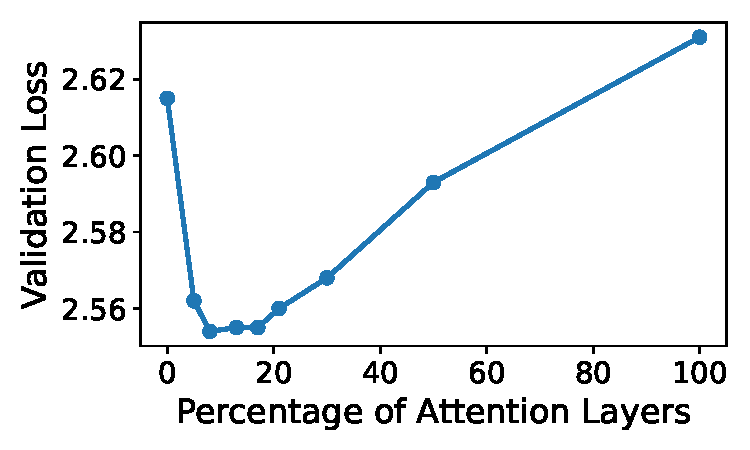
\includegraphics[width=\linewidth]{empirical-fig04-attention-ratio.pdf}
    \caption{Validation loss against percentage of attention layers.}
  \end{subfigure}\hfill
  \begin{subfigure}[b]{0.46\linewidth}
    \centering
    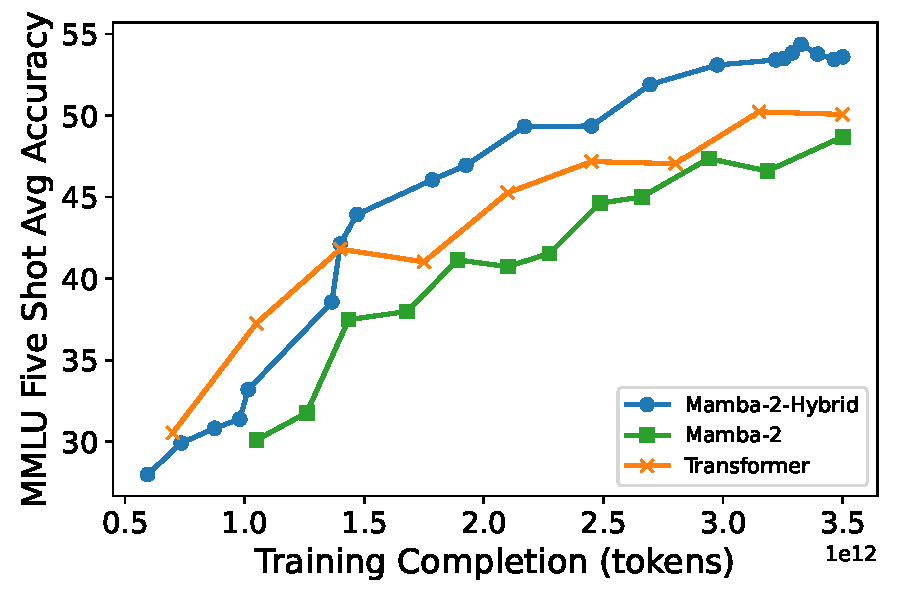
\includegraphics[width=\linewidth]{empirical-fig06-mmlu.pdf}
    \caption{Five-shot MMLU of 8B models during training.}
  \end{subfigure}
  \caption[How much attention a hybrid model needs]{How much attention a hybrid
  needs, and what it buys. \source{Waleffe et al.\
  (2024)~\cite{waleffe2024empirical}, Figs.~4 and~6}}
  \label{fig:attn-ratio}
\end{figure}

\section{The Nemotron Lineage}

\emph{Nemotron-H}~\cite{nvidia2025nemotronh} turned this finding into 8B and
56B models with about 8\% evenly dispersed attention layers
(Figure~\ref{fig:nemotronh}), matching Qwen-2.5 and Llama-3.1 while being up to
3$\times$ faster. \emph{Nemotron Nano~2}~\cite{nvidia2025nano2} applied it to a
reasoning model with up to 6$\times$ the throughput of Qwen3-8B.
\emph{\NN}~\cite{nvidia2025nano3}, the first Nemotron~3
model~\cite{nvidia2025nemotron3}, added MoE (31.6B total, 3.2B active) and
reached up to 3.3$\times$ the throughput of similar models
(Figure~\ref{fig:nano3}), but used a standard MoE and BF16 training.

\begin{figure}[!htbp]
  \centering
  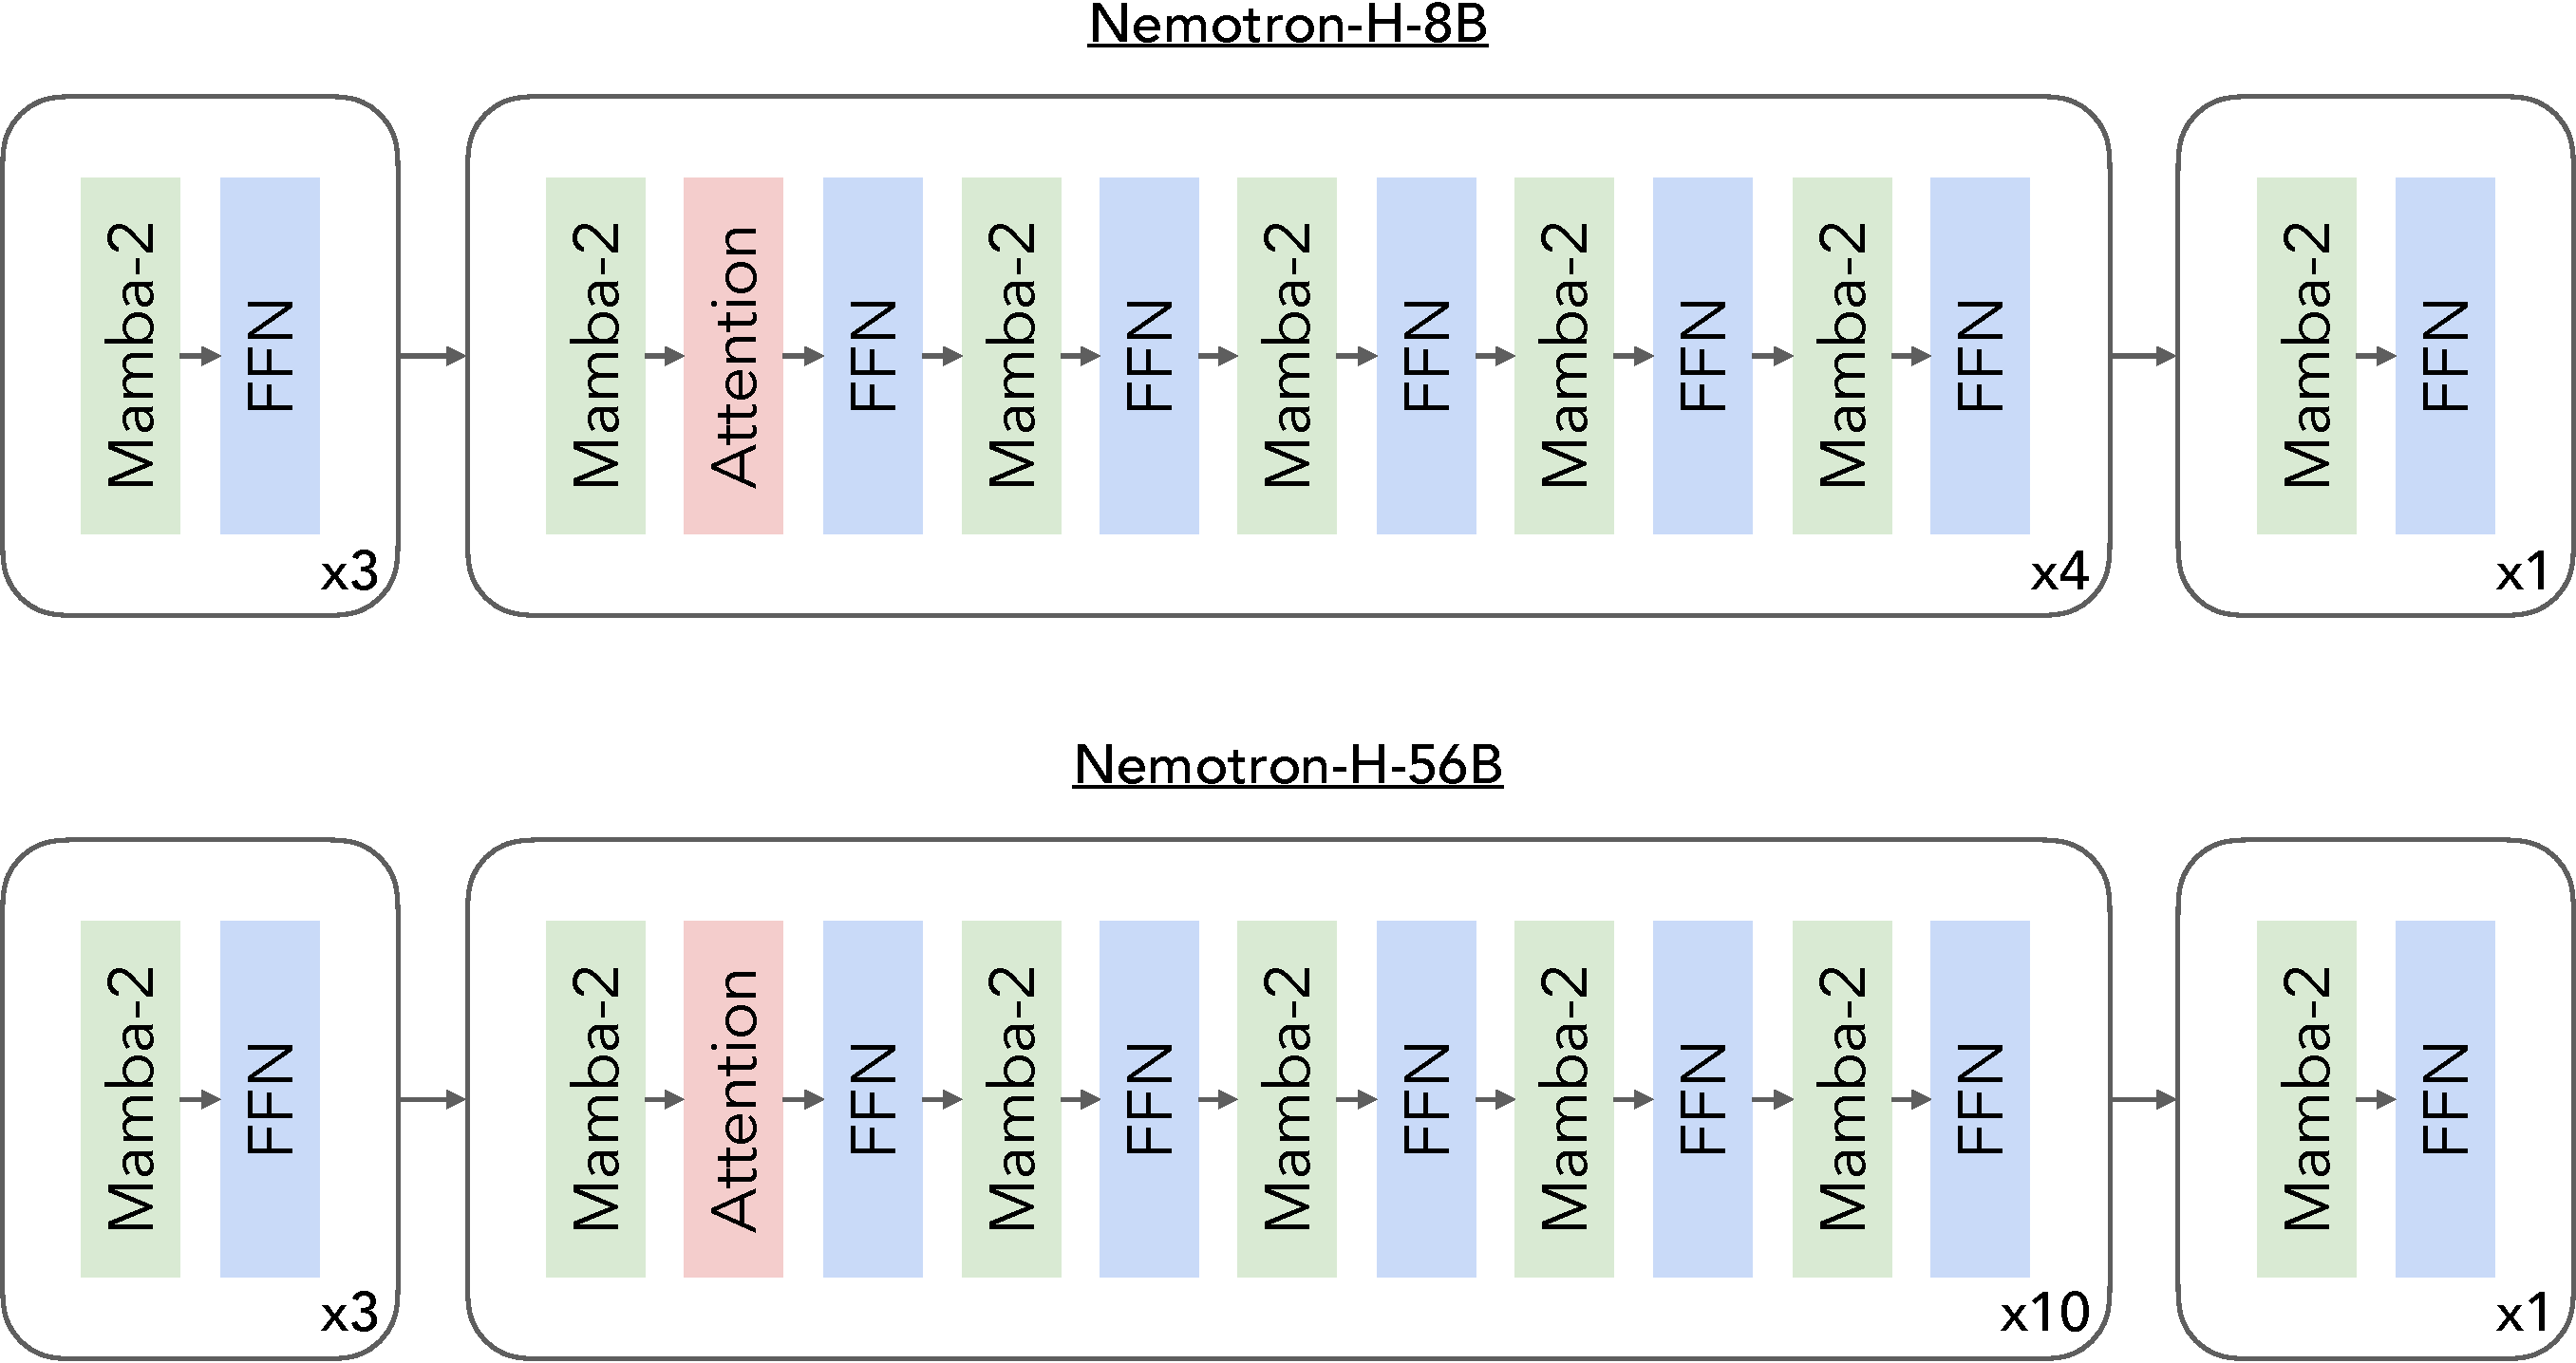
\includegraphics[width=0.8\linewidth]{nemotronh-fig02-layer-pattern.pdf}\\[4pt]
  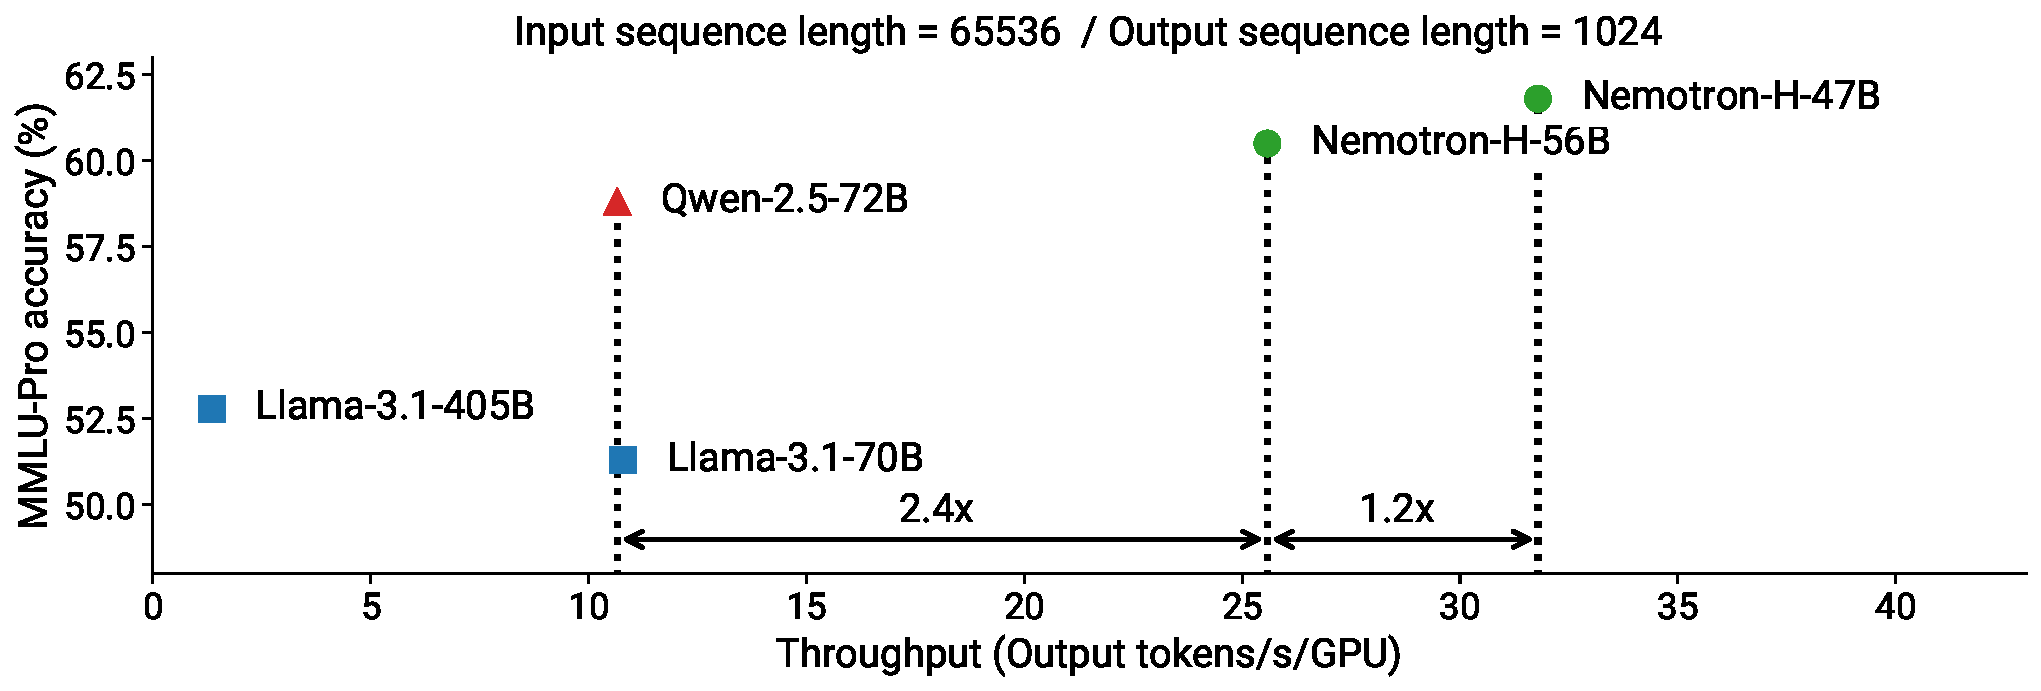
\includegraphics[width=0.8\linewidth]{nemotronh-fig01-throughput.pdf}
  \caption[Nemotron-H layer pattern and accuracy versus throughput]{Top:
  Nemotron-H layer patterns. Bottom: MMLU-Pro accuracy against inference
  throughput. \source{NVIDIA (2025)~\cite{nvidia2025nemotronh}, Figs.~2 and~1}}
  \label{fig:nemotronh}
\end{figure}

\begin{figure}[!htbp]
  \centering
  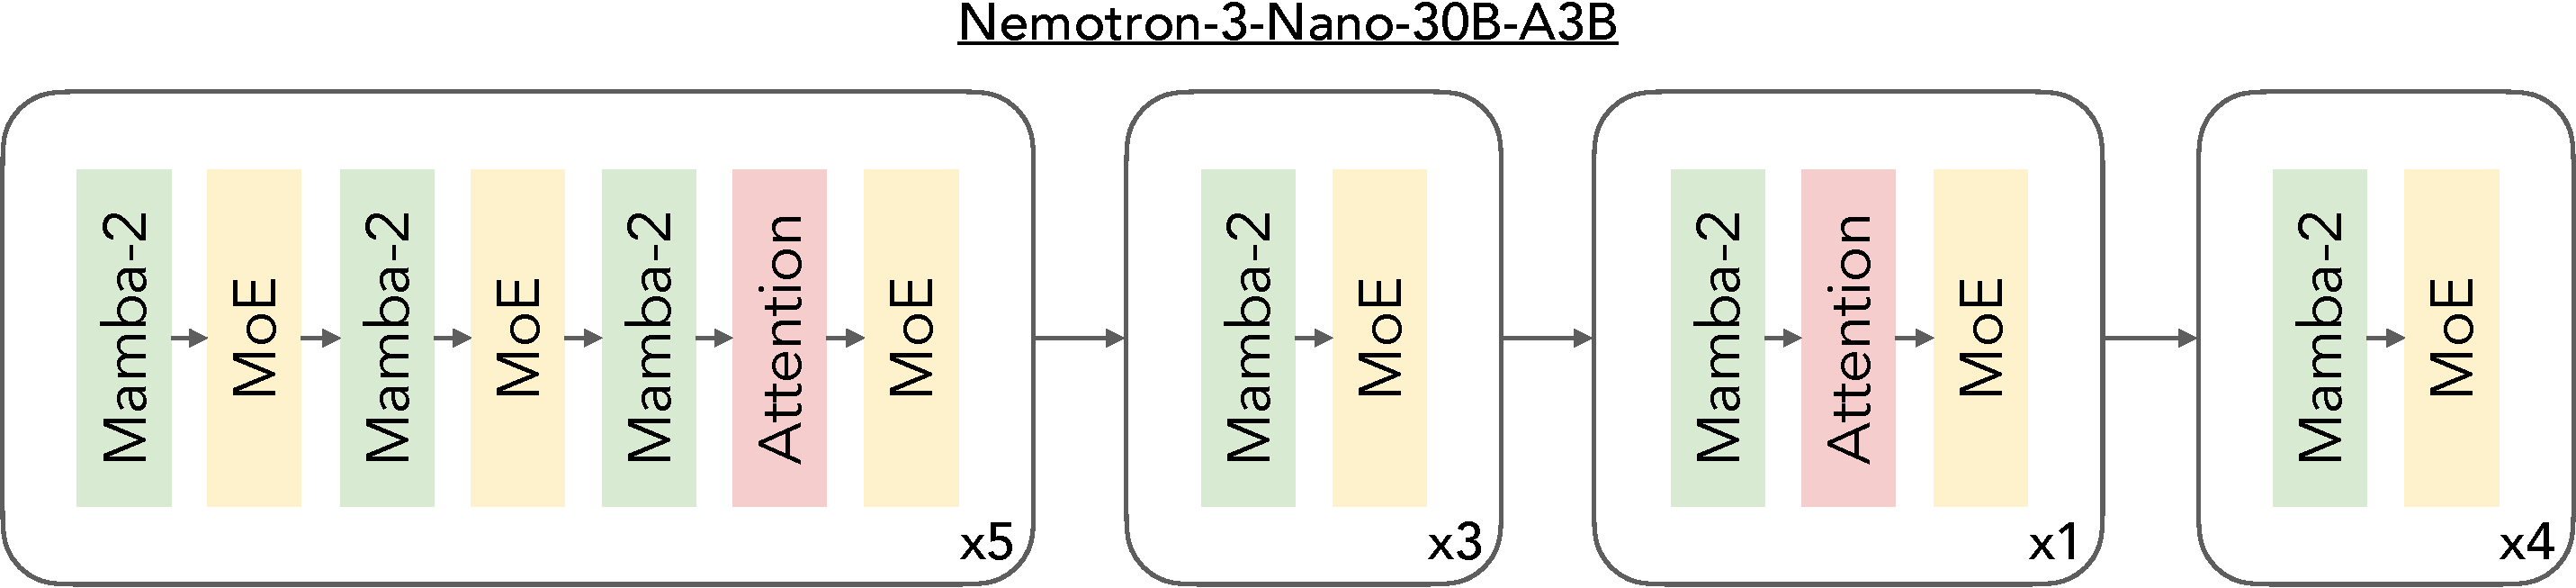
\includegraphics[width=0.78\linewidth]{nano3-fig02-layer-pattern.pdf}\\[4pt]
  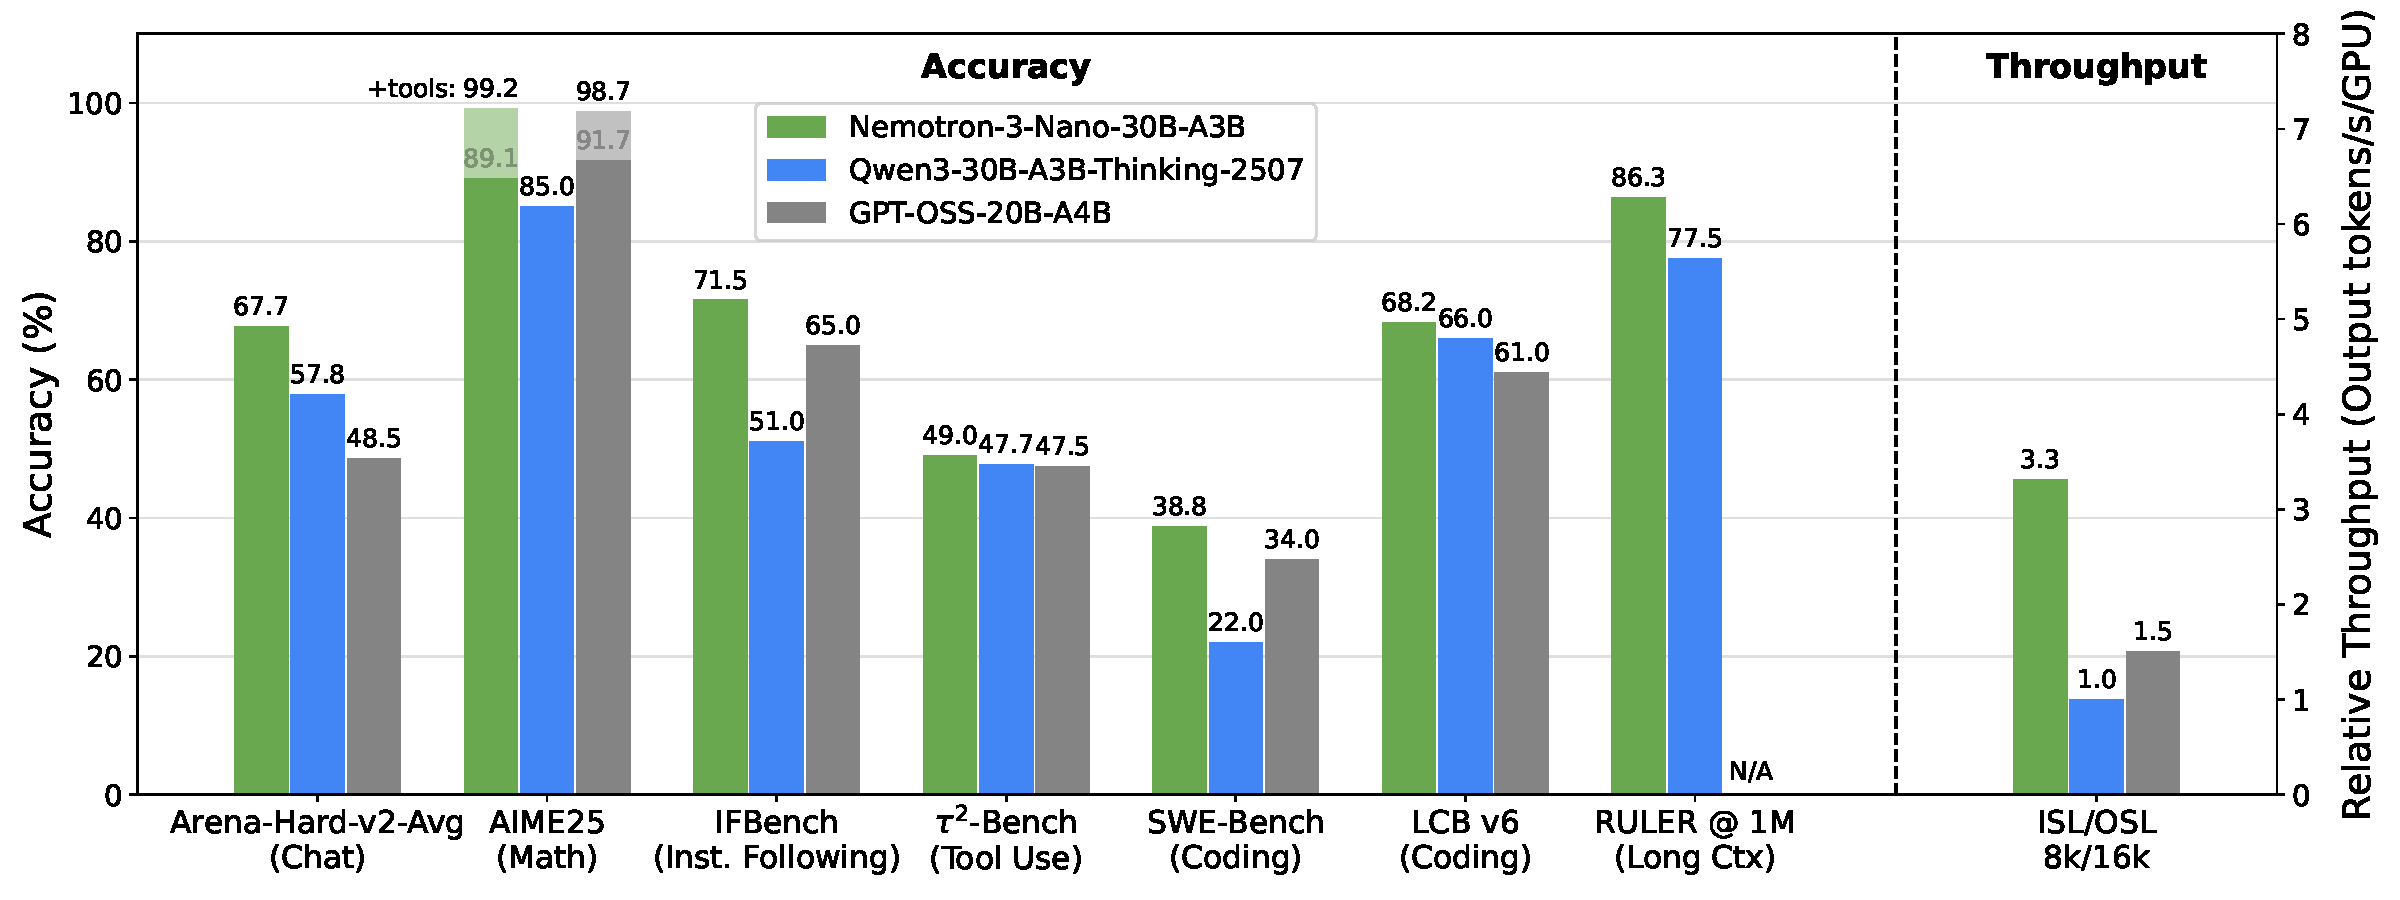
\includegraphics[width=0.88\linewidth]{nano3-fig01-accuracy-throughput.pdf}
  \caption[Nemotron 3 Nano layer pattern and accuracy/throughput comparison]{Top:
  \NN\ layer pattern. Bottom: accuracy and throughput against Qwen3-30B-A3B and
  GPT-OSS-20B. \source{NVIDIA (2025)~\cite{nvidia2025nano3}, Figs.~2 and~1}}
  \label{fig:nano3}
\end{figure}

\section{Supporting Techniques}

\textbf{Mixture-of-Experts.} The sparsely-gated MoE~\cite{shazeer2017moe} was
scaled by GShard~\cite{lepikhin2020gshard} and refined by
DeepSeek-V3~\cite{deepseek2024v3} with fine-grained experts and
auxiliary-loss-free balancing. LatentMoE~\cite{elango2026latentmoe} moves the
experts into a lower-dimensional latent space and is used in \NS.

\textbf{Multi-token prediction.} Gloeckle et al.~\cite{gloeckle2024mtp}
trained models to predict several future tokens with extra heads on a shared
trunk (Figure~\ref{fig:mtp-meta}), which pairs naturally with speculative
decoding~\cite{leviathan2022speculative,chen2023speculative}.

\textbf{Low-precision training.} NVFP4~\cite{nvidia2025nvfp4} showed stable
4-bit pretraining of a 12B model over 10 trillion tokens.

\begin{figure}[!htbp]
  \centering
  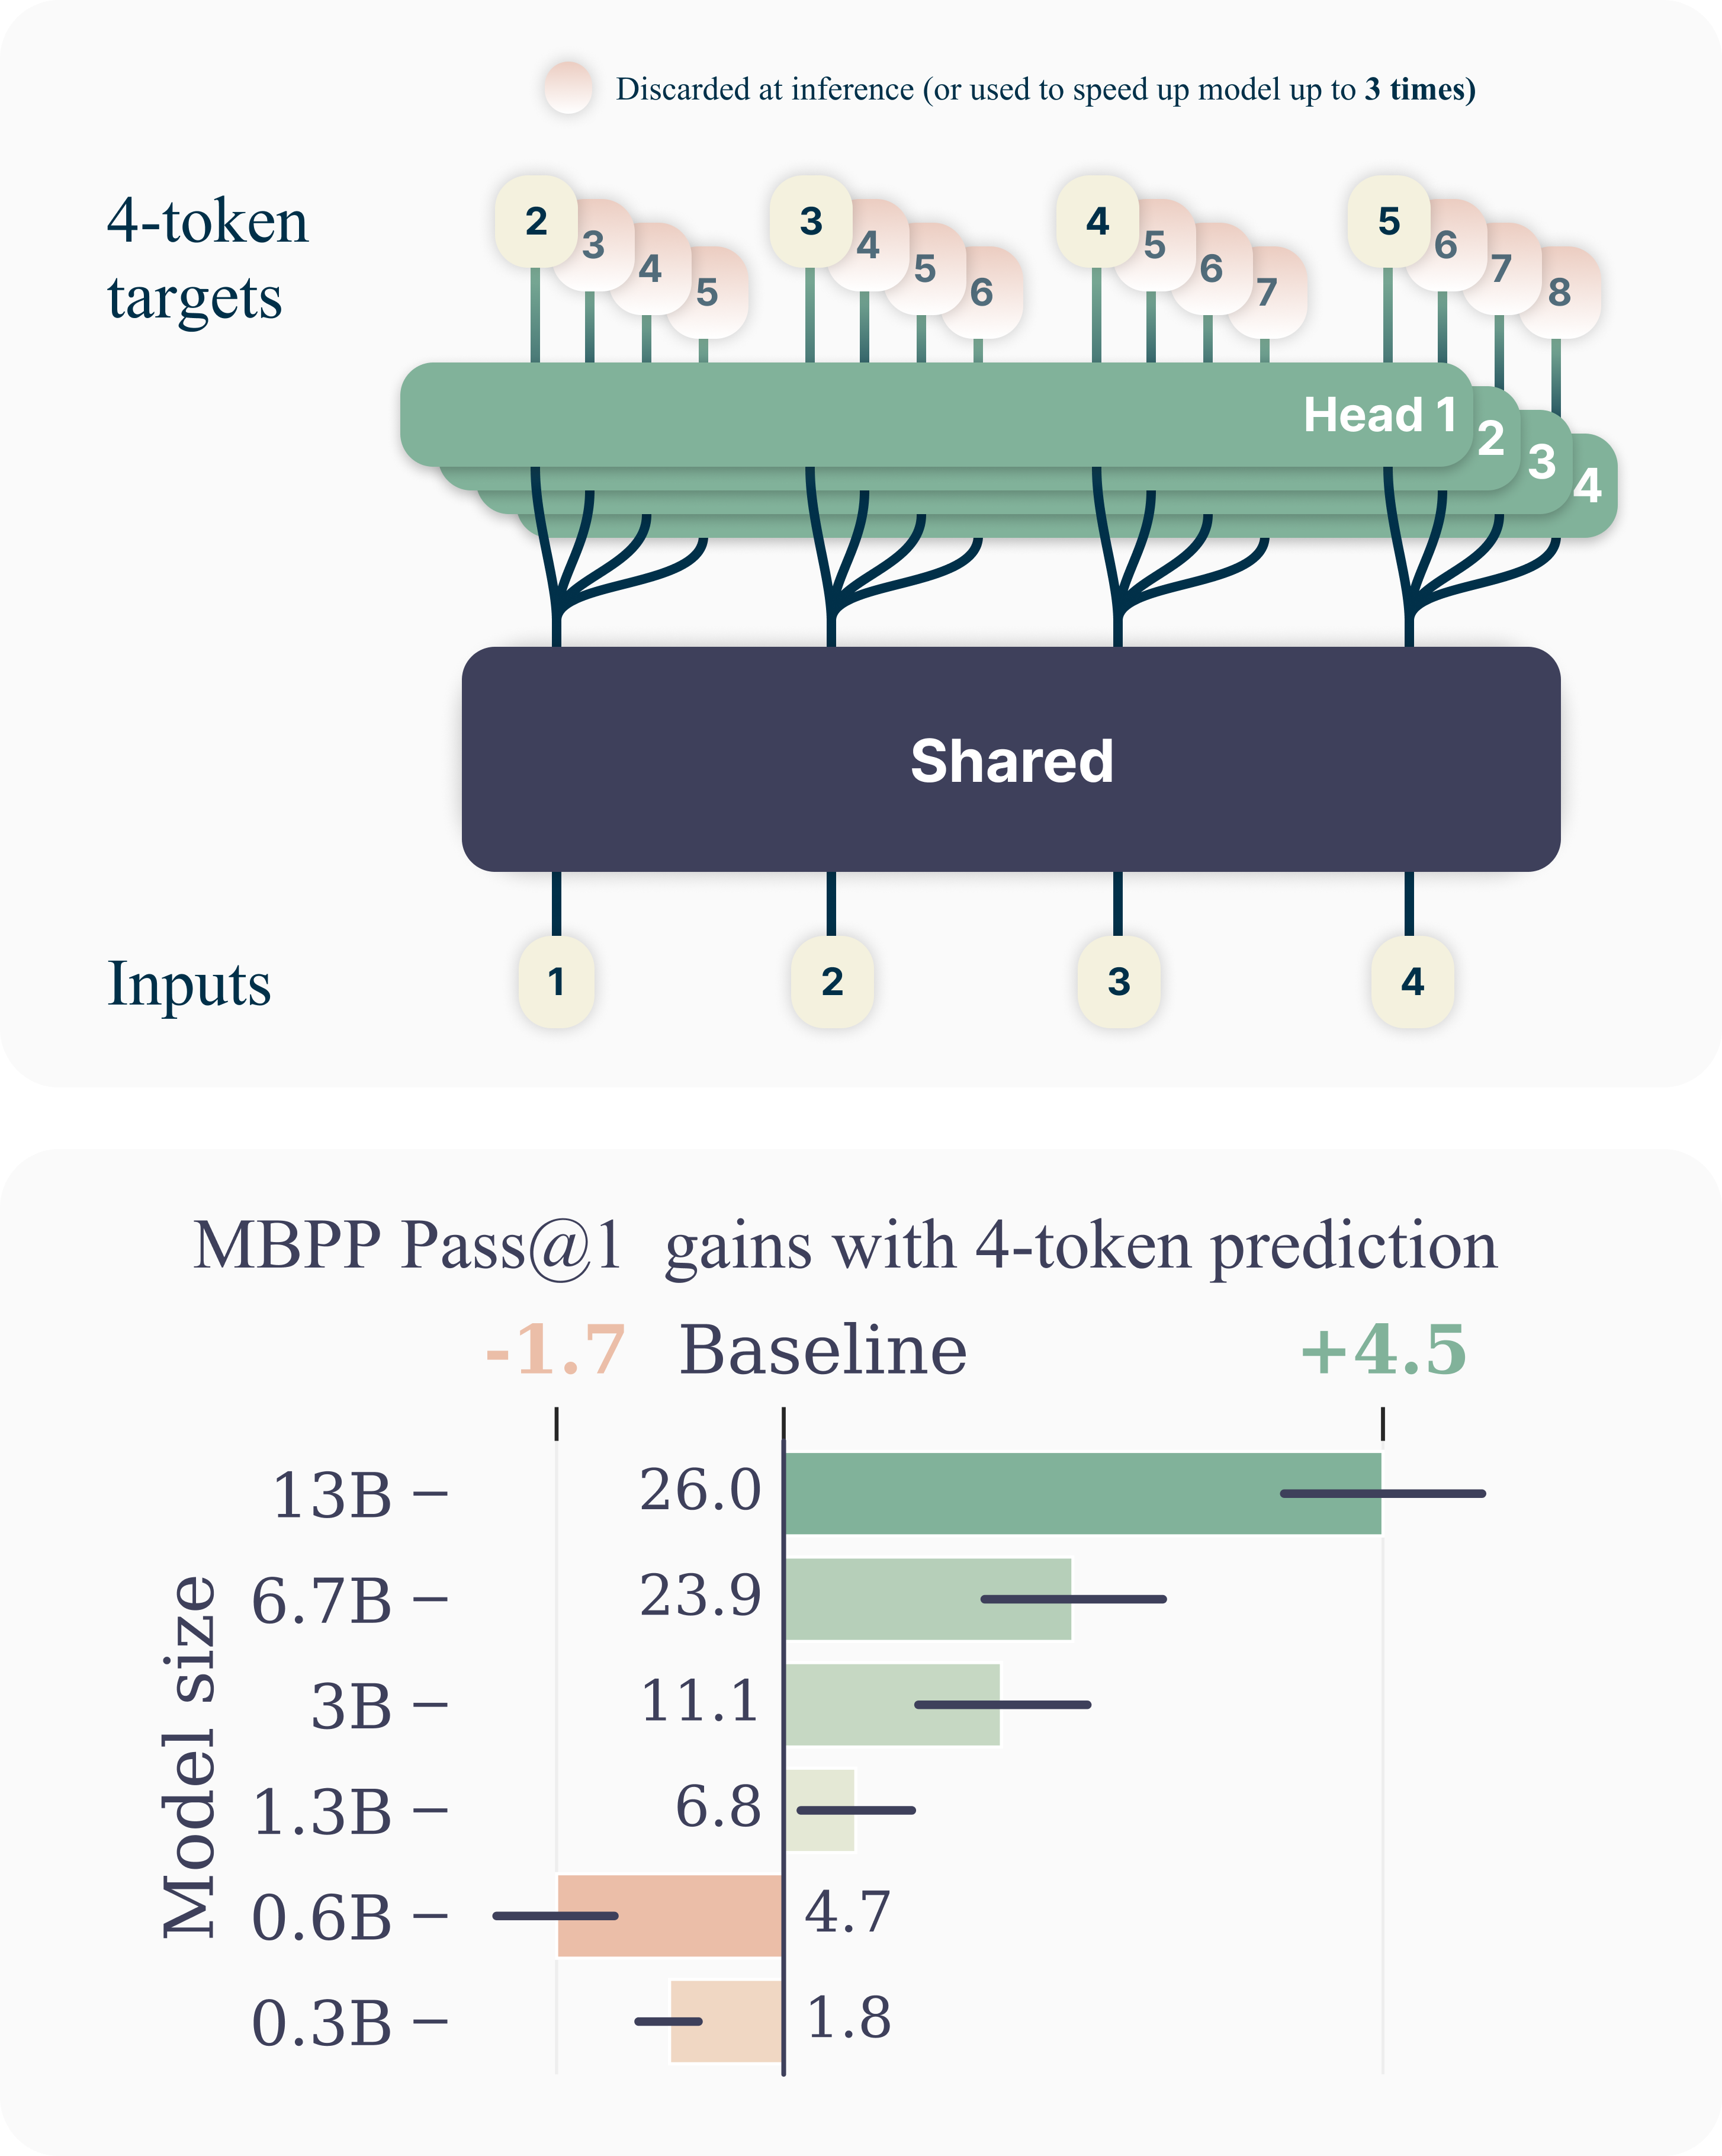
\includegraphics[width=0.48\linewidth]{mtp-fig01-overview.png}
  \caption[Multi-token prediction with several output heads on a shared trunk]{Multi-token
  prediction with several output heads on a shared trunk.
  \source{Gloeckle et al.\ (2024)~\cite{gloeckle2024mtp}, Fig.~1}}
  \label{fig:mtp-meta}
\end{figure}

\section{Summary of the Survey}

Table~\ref{tab:survey} summarises the main works and the gap each leaves open.

\begin{table}[!htbp]
\centering
\small
\caption{Summary of the literature survey}
\label{tab:survey}
\begin{tabularx}{\linewidth}{@{}P{3.0cm}LL@{}}
\toprule
\textbf{Study} & \textbf{Main contribution} & \textbf{Limitation / gap} \\
\midrule
Vaswani et al.\ (2017) \cite{vaswani2017attention} &
Transformer built on self-attention. &
Quadratic compute; KV cache grows with context. \\
Gu and Dao (2023) \cite{gu2023mamba} &
Mamba: selective, linear-time SSM. &
Fixed-size state; small to medium scale. \\
Dao and Gu (2024) \cite{dao2024mamba2} &
Mamba-2 and SSD; 2--8$\times$ faster layer. &
State is a lossy summary. \\
Lieber et al.\ (2024) \cite{lieber2024jamba} &
Jamba: first large hybrid with MoE. &
One fixed ratio; standard MoE. \\
Waleffe et al.\ (2024) \cite{waleffe2024empirical} &
Hybrid with $\sim$8\% attention beats a Transformer. &
Dense models only. \\
NVIDIA (2025) \cite{nvidia2025nano3} &
\NN: hybrid plus MoE at 30B. &
Small scale; standard MoE, BF16. \\
NVIDIA (2026) \cite{nvidia2026super} &
\NS: 120B with LatentMoE, MTP and NVFP4. &
Large memory; trails Qwen3.5 on some tasks. \\
\bottomrule
\end{tabularx}
\end{table}

\section{Research Gap}

The survey shows a clear progression. Mamba and Mamba-2 solved the cost of
long sequences but lost exact recall; Jamba and the empirical study of Waleffe
et al.\ showed that a small share of attention restores it; and the Nemotron-H,
Nano~2 and \NN\ models proved the idea in practice up to about 30 billion
parameters. What remained open was whether such a hybrid could be scaled to
more than one hundred billion parameters, combined with a hardware-aware MoE,
trained in 4-bit precision and post-trained for demanding agentic tasks while
staying competitive with the best Transformers. \NS\ is the first open model
to attempt all of these together, which is why it was chosen for this seminar.

\chapter{Background}
\label{ch:background}

This chapter introduces the three building blocks needed to understand \NS:
the Transformer with its KV cache, state-space models (Mamba and Mamba-2), and
Mixture-of-Experts layers.

\section{The Transformer and the KV Cache}

\subsection{Self-Attention}

A Transformer layer consists of a self-attention block followed by a
feed-forward network (FFN)~\cite{vaswani2017attention}. Given a sequence of $n$
token representations stacked as the rows of $X \in \mathbb{R}^{n \times d}$,
self-attention forms queries, keys and values by linear projection,
$Q = XW_Q$, $K = XW_K$, $V = XW_V$, and computes
\begin{equation}
  \operatorname{Attention}(Q,K,V) =
  \operatorname{softmax}\!\left(\frac{QK^{\top}}{\sqrt{d_k}}\right)V ,
  \label{eq:attention}
\end{equation}
where $d_k$ is the dimension of each key. The matrix $QK^{\top}$ has $n \times
n$ entries, one for every pair of tokens. This is what gives attention its
power---any token can retrieve information from any other token in a single
step---and also what makes it expensive: both the time and the memory of this
product grow as $O(n^2)$. Doubling the input length quadruples the work in
every attention layer. Figure~\ref{fig:complexity} contrasts this growth with
the linear growth of a state-space layer.

\begin{figure}[htbp]
  \centering
  % Attention O(n^2) vs Mamba O(n): relative per-layer cost against sequence length
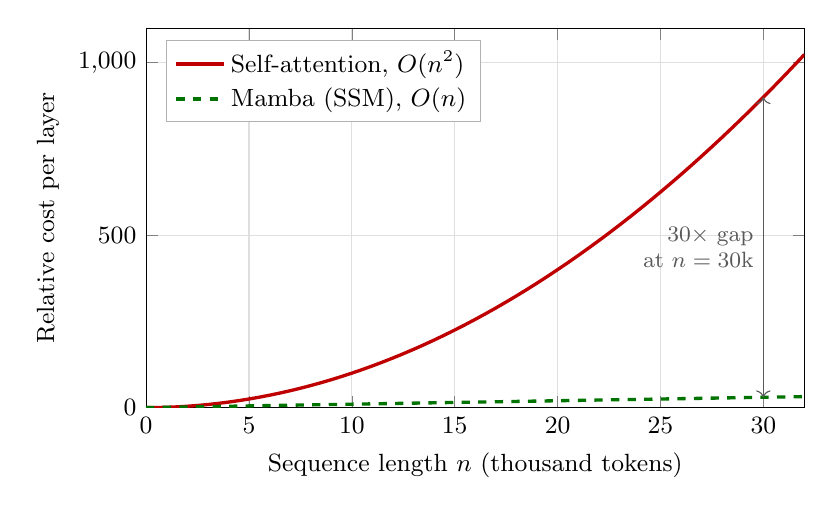
\begin{tikzpicture}
\begin{axis}[
  width=0.82\linewidth, height=6.4cm,
  xlabel={Sequence length $n$ (thousand tokens)},
  ylabel={Relative cost per layer},
  xmin=0, xmax=32, ymin=0, ymax=1100,
  domain=0:32, samples=65,
  grid=major, grid style={gray!25},
  legend pos=north west, legend cell align=left,
  legend style={font=\small, draw=gray!60},
  tick label style={font=\small}, label style={font=\small}]
\addplot[very thick, red!75!black] {x^2};
\addlegendentry{Self-attention, $O(n^2)$}
\addplot[very thick, green!45!black, dashed] {x};
\addlegendentry{Mamba (SSM), $O(n)$}
\draw[<->, gray!70!black] (axis cs:30,30) -- (axis cs:30,900)
  node[midway, left, font=\footnotesize, align=right] {$30\times$ gap\\at $n=30$k};
\end{axis}
\end{tikzpicture}

  \caption[Quadratic cost of self-attention versus linear cost of Mamba]{Relative
  per-layer cost of self-attention, $O(n^2)$, and of a Mamba layer, $O(n)$, as
  the sequence grows (both normalised to 1 at $n=1$k tokens; drawn by the
  author).}
  \label{fig:complexity}
\end{figure}

\subsection{Autoregressive Generation and the KV Cache}

Language models generate text one token at a time. To produce token $t+1$ the
newest token must attend to all $t$ tokens before it. Recomputing the keys and
values of those earlier tokens at every step would be wasteful, so
implementations store them in a \emph{KV cache} and append one new key--value
pair per layer for every generated token. The cache removes redundant
computation, but it introduces two costs that grow with the context:
\begin{itemize}
  \item \textbf{Memory.} The cache holds one entry per past token per attention
        layer, so its size grows linearly and without bound as the context
        lengthens.
  \item \textbf{Time per token.} Every new token must read the whole cache, so
        the cost of generating a token also grows linearly with the context,
        and the total cost of generating a sequence grows quadratically.
\end{itemize}
More cache means more GPU memory and more memory traffic per token, so fewer
requests fit on a GPU and each one runs more slowly. Figure~\ref{fig:kvcache}
illustrates the difference from a state-space layer, whose state does not grow.

\begin{figure}[htbp]
  \centering
  % KV cache growth vs constant-size SSM state during generation
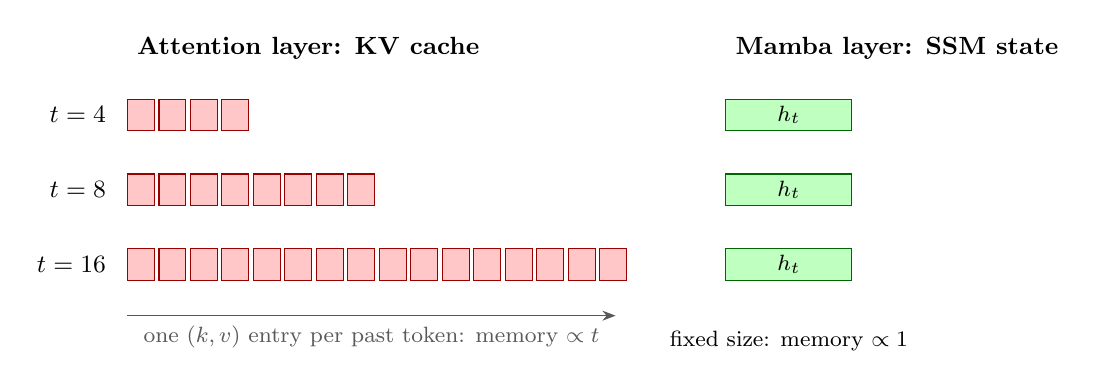
\begin{tikzpicture}[font=\small]
\node[font=\small\bfseries, anchor=west] at (0,0.85) {Attention layer: KV cache};
\node[font=\small\bfseries, anchor=west] at (7.6,0.85) {Mamba layer: SSM state};
\foreach \n/\y/\lab in {4/0/{$t=4$}, 8/-0.95/{$t=8$}, 16/-1.9/{$t=16$}}{
  \node[anchor=east] at (-0.15,\y) {\lab};
  \foreach \i in {1,...,\n}{
    \draw[fill=red!22, draw=red!60!black] ({(\i-1)*0.4},{\y-0.2}) rectangle ++(0.34,0.4);
  }
  \draw[fill=green!25, draw=green!40!black] (7.6,{\y-0.2}) rectangle ++(1.6,0.4);
  \node[font=\footnotesize] at (8.4,\y) {$h_t$};
}
\draw[-{Stealth}, gray!70!black] (0,-2.55) -- (6.2,-2.55)
  node[midway, below, font=\footnotesize] {one $(k,v)$ entry per past token: memory $\propto t$};
\node[font=\footnotesize, anchor=north] at (8.4,-2.62) {fixed size: memory $\propto 1$};
\end{tikzpicture}

  \caption[KV cache growth versus a constant-size SSM state]{During generation
  an attention layer appends one key--value entry per token, whereas a Mamba
  layer overwrites a state of fixed size (drawn by the author).}
  \label{fig:kvcache}
\end{figure}

Techniques such as Grouped-Query Attention~\cite{ainslie2023gqa}, in which
many query heads share a small number of key--value heads, reduce the size of
each cache entry but not the way the cache scales. For very long-context tasks
a pure Transformer therefore remains expensive and inefficient.

\section{State-Space Models}

\subsection{From Continuous Systems to Sequence Layers}

A state-space model describes a system through a hidden state $h(t) \in
\mathbb{R}^{N}$ that evolves under an input signal $x(t)$ and produces an
output $y(t)$:
\begin{equation}
  h'(t) = A\,h(t) + B\,x(t), \qquad y(t) = C^{\top} h(t).
  \label{eq:ssm-cont}
\end{equation}
To apply this to a sequence of tokens, the system is discretised with a step
size $\Delta$. Under the commonly used zero-order hold rule the discrete
parameters are $\bar{A} = \exp(\Delta A)$ and
$\bar{B} = (\Delta A)^{-1}\bigl(\exp(\Delta A) - I\bigr)\,\Delta B$, which
gives the recurrence~\cite{gu2021s4,gu2023mamba}
\begin{equation}
  h_t = \bar{A}\,h_{t-1} + \bar{B}\,x_t, \qquad y_t = C^{\top} h_t .
  \label{eq:ssm-disc}
\end{equation}
In words, the model reads the text one token at a time and keeps one small
``note'' in memory, the state $h_t$. After each token it updates the note,
writing in what matters and letting the rest decay. The note has the same size
whether the text is one thousand or one million tokens long.
Figure~\ref{fig:ssm} shows this recurrence unrolled over three steps.

\begin{figure}[htbp]
  \centering
  % Unrolled state-space recurrence  h_t = A_t h_{t-1} + B_t x_t,  y_t = C_t^T h_t
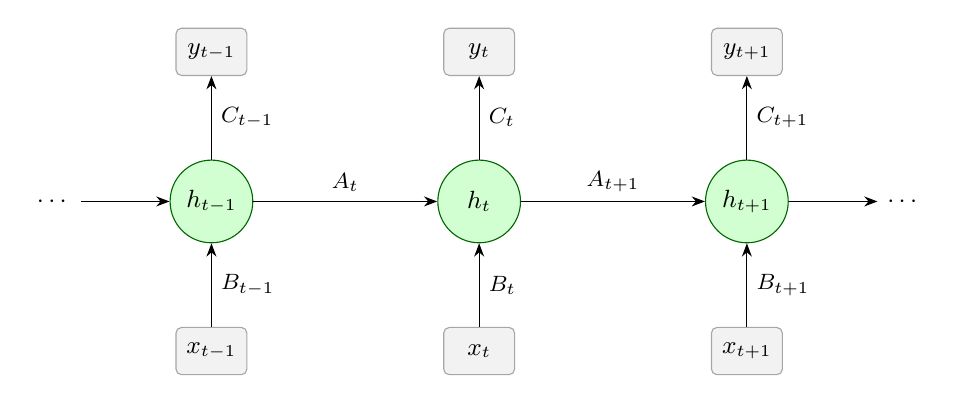
\begin{tikzpicture}[
  font=\small, >={Stealth},
  state/.style={circle, draw=green!40!black, fill=green!18, minimum size=1.05cm, inner sep=0pt},
  io/.style={rectangle, rounded corners=2pt, draw=gray!70, fill=gray!10, minimum width=0.9cm, minimum height=0.6cm}]
\node[state] (h0) at (0,0)   {$h_{t-1}$};
\node[state] (h1) at (3.4,0) {$h_{t}$};
\node[state] (h2) at (6.8,0) {$h_{t+1}$};
\node (l) at (-2.0,0) {$\cdots$};
\node (r) at (8.8,0)  {$\cdots$};
\foreach \k/\x/\lab in {0/0/{t-1}, 1/3.4/{t}, 2/6.8/{t+1}}{
  \node[io] (x\k) at (\x,-1.9) {$x_{\lab}$};
  \node[io] (y\k) at (\x,1.9)  {$y_{\lab}$};
  \draw[->] (x\k) -- node[right, font=\footnotesize] {$B_{\lab}$} (h\k);
  \draw[->] (h\k) -- node[right, font=\footnotesize] {$C_{\lab}$} (y\k);
}
\draw[->] (l) -- (h0);
\draw[->] (h0) -- node[above, font=\footnotesize] {$A_{t}$} (h1);
\draw[->] (h1) -- node[above, font=\footnotesize] {$A_{t+1}$} (h2);
\draw[->] (h2) -- (r);
\end{tikzpicture}

  \caption[Unrolled state-space recurrence]{The state-space recurrence unrolled
  over time: each state $h_t$ depends only on the previous state and the
  current input (drawn by the author).}
  \label{fig:ssm}
\end{figure}

Because the update in Eq.~\eqref{eq:ssm-disc} touches only $h_{t-1}$ and $x_t$,
processing $n$ tokens costs $O(n)$ time, and generating a new token costs the
same amount of work and memory no matter how long the context already is.

\subsection{Mamba: Selective State Spaces}

In early SSMs such as S4~\cite{gu2021s4} the matrices $A$, $B$ and $C$ are
fixed after training, so every token is written into the state in the same
way. Text is not like that: some tokens are essential and many are filler.
Mamba~\cite{gu2023mamba} makes the parameters depend on the current input,
\begin{equation}
  h_t = \bar{A}(x_t)\,h_{t-1} + \bar{B}(x_t)\,x_t, \qquad
  y_t = C(x_t)^{\top} h_t ,
  \label{eq:mamba}
\end{equation}
so that the model can \emph{select} what to remember. When $\bar{A}(x_t)$ is
close to the identity and $\bar{B}(x_t)$ is small, the token is effectively
ignored and the state is carried forward unchanged; in the opposite case the
state is reset and overwritten. The Mamba block wraps this selective SSM with a
linear projection, a short convolution and a gated branch
(Figure~\ref{fig:mamba-block}) and is stacked like a Transformer block, without
any attention.

\begin{figure}[htbp]
  \centering
  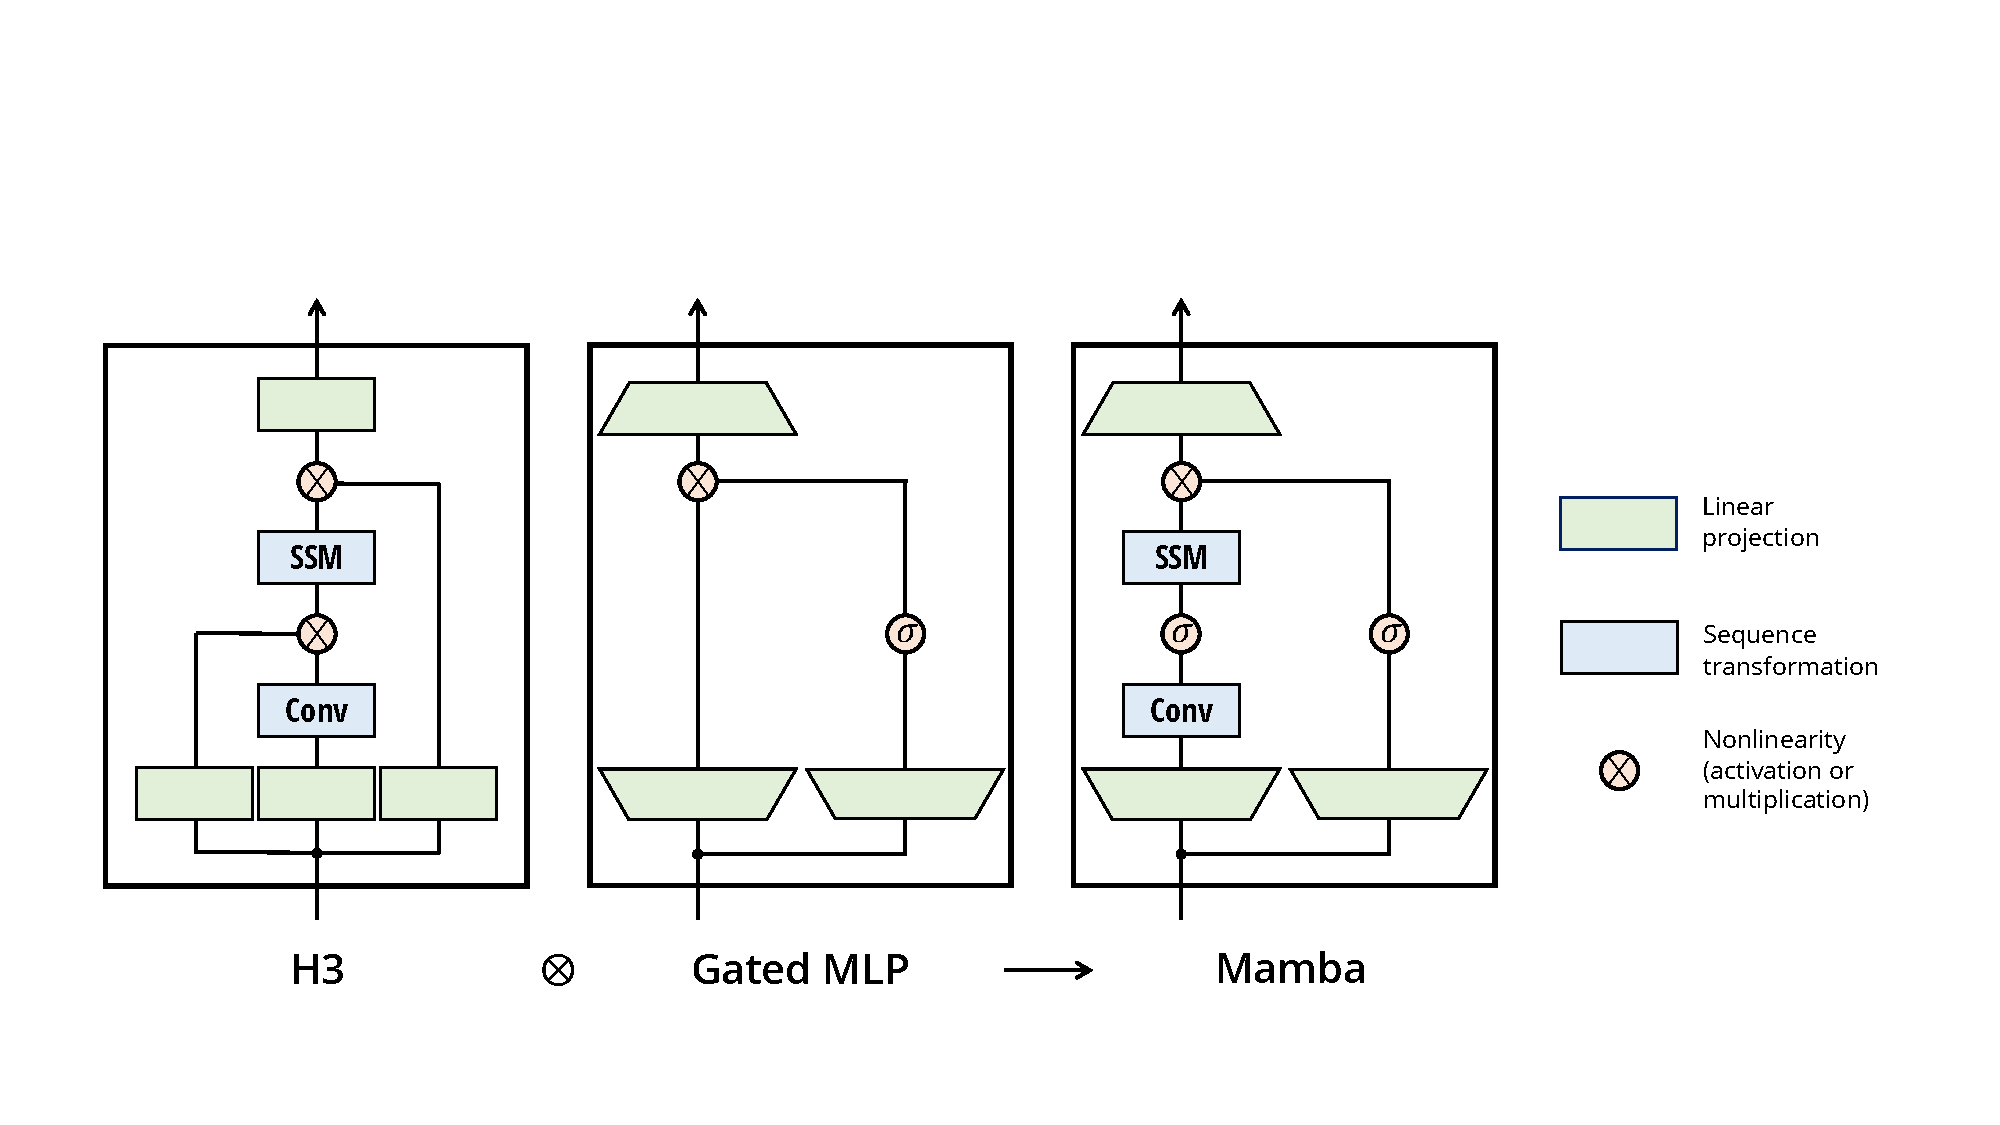
\includegraphics[width=0.9\linewidth]{mamba-fig03-block.pdf}
  \caption[The Mamba block compared with the H3 and gated-MLP blocks]{The Mamba
  block combines the H3 block, the basis of most earlier SSM architectures,
  with the gated MLP block. \source{Gu and Dao (2023)~\cite{gu2023mamba}, Fig.~3}}
  \label{fig:mamba-block}
\end{figure}

\subsection{Mamba-2 and State Space Duality}
\label{sec:mamba2}

Mamba-2~\cite{dao2024mamba2} starts from an observation about
Eq.~\eqref{eq:mamba}. Unrolling the recurrence shows that the whole layer is a
single matrix multiplication $y = Mx$, where
\begin{equation}
  M_{ji} = C_j^{\top} A_j A_{j-1} \cdots A_{i+1} B_i \quad (j \ge i),
  \label{eq:ssd}
\end{equation}
and $M_{ji}=0$ for $j<i$. Matrices of this form are called
\emph{semiseparable}. Dao and Gu show that a restricted form of masked
attention produces exactly the same family of matrices, which they call
\emph{structured state space duality} (SSD): the same sequence transformation
can be computed either as a linear-time recurrence (the SSM view) or as a
matrix product (the attention view).

Mamba-2 exploits both views. It restricts each $A_t$ to a scalar times the
identity and groups channels into \emph{heads}, much like attention heads.
During training, the sequence is cut into chunks; within a chunk the layer is
computed with ordinary matrix multiplications, which GPUs execute very
efficiently, and the states are passed between chunks with the recurrence. As
a result the SSD algorithm is 2--8$\times$ faster than Mamba's sequential scan
while keeping linear scaling in sequence length. During generation Mamba-2
falls back to the pure recurrence and so keeps a constant-size state. The block
is also simplified (Figure~\ref{fig:mamba2-block}), which makes it easier to
parallelise across GPUs.

\begin{figure}[htbp]
  \centering
  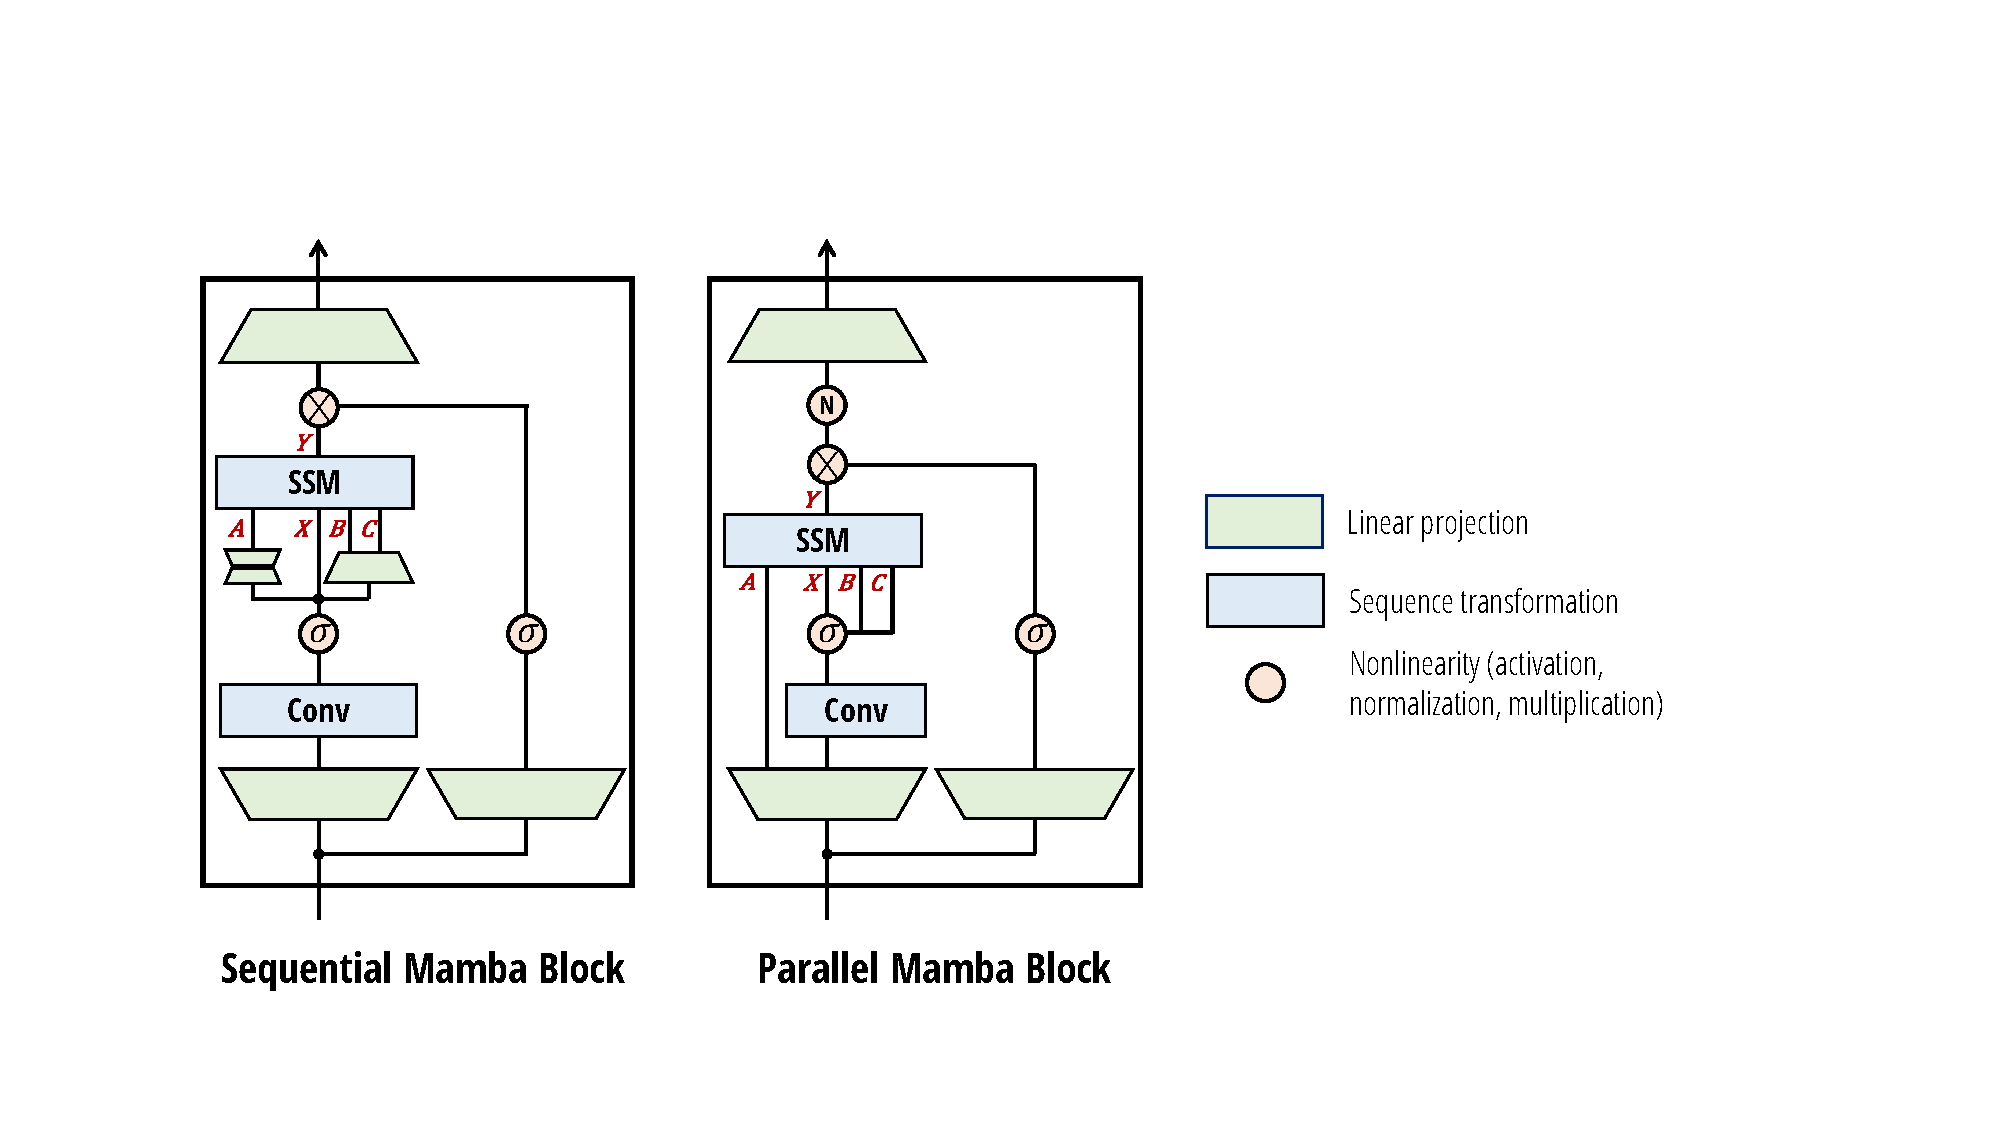
\includegraphics[width=0.78\linewidth]{mamba2-fig06-block.pdf}
  \caption[The Mamba-2 block]{The Mamba-2 block simplifies the Mamba block by
  removing sequential linear projections; the SSM parameters are produced in
  parallel at the start of the block. \source{Dao and Gu
  (2024)~\cite{dao2024mamba2}, Fig.~6}}
  \label{fig:mamba2-block}
\end{figure}

\subsection{What a State-Space Layer Cannot Do}

The strength of an SSM is also its weakness. Everything the layer knows about
the past must fit into a state of fixed size, so the state is necessarily a
lossy summary. Tasks that need an exact copy of something seen long ago---a
phone number from a long list, a variable name defined thousands of lines
earlier---are precisely where pure SSMs fall behind
Transformers~\cite{waleffe2024empirical}. Attention has the opposite profile:
perfect recall at high cost. Table~\ref{tab:attn-vs-ssm} summarises the
contrast, which is the motivation for hybrid models.

\begin{table}[htbp]
\centering
\small
\caption{Self-attention and Mamba-2 layers compared}
\label{tab:attn-vs-ssm}
\begin{tabularx}{\linewidth}{@{}P{4.2cm}LL@{}}
\toprule
\textbf{Property} & \textbf{Self-attention} & \textbf{Mamba-2 (SSM)} \\
\midrule
Compute for $n$ tokens & $O(n^2)$ & $O(n)$ \\
Memory during generation & KV cache, grows as $O(n)$ & Fixed-size state, $O(1)$ \\
Work per generated token & Grows with context & Constant \\
Access to past tokens & Exact, to every token & Compressed summary \\
Typical weakness & Cost on long contexts & Exact recall and copying \\
\bottomrule
\end{tabularx}
\end{table}

\section{Mixture-of-Experts}

\subsection{The Basic Idea}

In a standard Transformer, roughly two thirds of the parameters sit in the
feed-forward networks, and every token passes through all of them. A
Mixture-of-Experts layer~\cite{shazeer2017moe} replaces the single FFN with
$N$ smaller FFNs called \emph{experts}, $E_1,\dots,E_N$, together with a small
\emph{router} network. For each token $x$ the router produces a score for every
expert, only the $k$ highest-scoring experts are evaluated, and their outputs
are combined:
\begin{equation}
  y = \sum_{i \,\in\, \operatorname{TopK}(g(x),\,k)} g_i(x)\, E_i(x),
  \qquad E_i(x) = W^{(i)}_{2}\,\sigma\!\bigl(W^{(i)}_{1}x\bigr).
  \label{eq:moe}
\end{equation}
Here $g(x)$ is the vector of router scores and $\sigma$ is a non-linearity.
Figure~\ref{fig:moe} sketches the layer. The experts that are not selected do
no work for this token, so the \emph{total} parameter count grows with $N$
while the \emph{active} parameter count and the FLOPs per token grow only with
$k$. This is how a model can be very large and still cheap to run.

\begin{figure}[htbp]
  \centering
  % Mixture-of-Experts layer: router scores all experts, only the top-k run
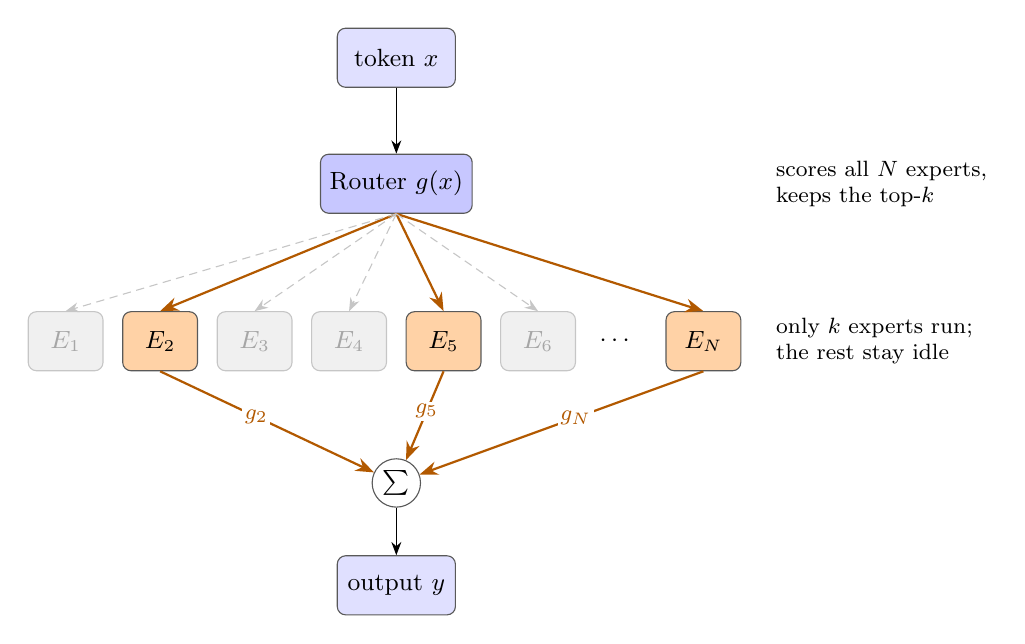
\begin{tikzpicture}[
  font=\small, >={Stealth},
  box/.style={rectangle, rounded corners=3pt, draw=gray!70!black, minimum height=0.75cm},
  on/.style={box, fill=orange!35, minimum width=0.95cm},
  off/.style={box, fill=gray!12, text=gray!70, draw=gray!45, minimum width=0.95cm}]
\node[box, fill=blue!12, minimum width=1.5cm] (x) at (0,0) {token $x$};
\node[box, fill=blue!22, minimum width=1.9cm, align=center] (r) at (0,-1.6) {Router $g(x)$};
\node[off] (e1) at (-4.2,-3.6) {$E_1$};
\node[on]  (e2) at (-3.0,-3.6) {$E_2$};
\node[off] (e3) at (-1.8,-3.6) {$E_3$};
\node[off] (e4) at (-0.6,-3.6) {$E_4$};
\node[on]  (e5) at (0.6,-3.6)  {$E_5$};
\node[off] (e6) at (1.8,-3.6)  {$E_6$};
\node (dots) at (2.8,-3.6) {$\cdots$};
\node[on]  (en) at (3.9,-3.6)  {$E_N$};
\node[circle, draw=gray!70!black, fill=white, inner sep=1.5pt] (s) at (0,-5.4) {$\sum$};
\node[box, fill=blue!12, minimum width=1.5cm] (y) at (0,-6.7) {output $y$};
\draw[->] (x) -- (r);
\foreach \e/\w in {e2/g_2, e5/g_5, en/g_N}{
  \draw[->, thick, orange!70!black] (r.south) -- (\e.north);
  \draw[->, thick, orange!70!black] (\e.south) -- node[pos=0.45, fill=white, inner sep=1pt, font=\footnotesize] {$\w$} (s);
}
\foreach \e in {e1,e3,e4,e6}{ \draw[->, gray!45, densely dashed] (r.south) -- (\e.north); }
\draw[->] (s) -- (y);
\node[font=\footnotesize, align=left, anchor=west] at (4.7,-1.6) {scores all $N$ experts,\\keeps the top-$k$};
\node[font=\footnotesize, align=left, anchor=west] at (4.7,-3.6) {only $k$ experts run;\\the rest stay idle};
\end{tikzpicture}

  \caption[Mixture-of-Experts layer with router and top-$k$ selection]{A
  Mixture-of-Experts layer: the router scores all $N$ experts and only the
  top-$k$ (shaded) are executed and summed (drawn by the author).}
  \label{fig:moe}
\end{figure}

\subsection{Practical Issues}

Sparse routing introduces problems that dense models do not have.
\begin{itemize}
  \item \textbf{Load balancing.} If the router sends most tokens to a few
        favourite experts, the rest are wasted. GShard~\cite{lepikhin2020gshard}
        adds an auxiliary loss that encourages even usage, and
        DeepSeek-V3~\cite{deepseek2024v3} adjusts a per-expert bias instead so
        that no extra loss term is needed.
  \item \textbf{Memory.} Idle experts still occupy memory. All $N$ experts
        must be loaded even though only $k$ run for a given token.
  \item \textbf{Memory bandwidth and communication.} Each token may use a
        different set of experts, so the weights that must be read change from
        token to token, and in a multi-GPU deployment tokens must be shipped to
        whichever device holds their experts.
\end{itemize}
These hardware-level costs are the starting point for LatentMoE, the MoE
variant used in \NS, which is described in Chapter~\ref{ch:arch}.

\chapter{Nemotron 3 Super Architecture}
\label{ch:arch}

\section{Overview}

\NS\ 120B-A12B~\cite{nvidia2026super} has 120.6 billion parameters in total
and 12.7 billion active per token. It scales up the hybrid Mamba--attention MoE
design of \NN~\cite{nvidia2025nano3} and is the first model in the family to
use \textbf{LatentMoE}, \textbf{Multi-Token Prediction (MTP)} for native
speculative decoding, and \textbf{NVFP4} pretraining
(Chapter~\ref{ch:training}). Table~\ref{tab:arch} lists its main dimensions.

\begin{table}[!htbp]
\centering
\small
\caption[Architectural dimensions of Nemotron 3 Super]{Architectural dimensions
of \NS\ (from~\cite{nvidia2026super}, Table~1)}
\label{tab:arch}
\begin{tabular}{@{}lr@{\hspace{2.5em}}lr@{}}
\toprule
\textbf{Configuration} & \textbf{Value} & \textbf{Configuration} & \textbf{Value} \\
\midrule
Total layers & 88 & Mamba heads / head dim. & 128 / 64 \\
Hidden dimension $d$ & 4096 & Mamba state dimension & 128 \\
Attention query heads & 32 & Experts per layer $N$ & 512 \\
Attention KV heads & 2 & Active experts (top-$k$) & 22 \\
Attention head dimension & 128 & Expert hidden dimension & 2688 \\
MTP layers (shared) & 2 & MoE latent size $\ell$ & 1024 \\
\bottomrule
\end{tabular}
\end{table}

\section{Hybrid Interleaved Layout}

Every sequence mixer---a Mamba-2 block or, occasionally, an attention
block---is followed by a LatentMoE layer (Figure~\ref{fig:layer-pattern}). Of
the 88 layers, 40 are Mamba-2, 40 are LatentMoE and only 8 are attention
layers, about 9\% of the stack, in line with the roughly 8\% found optimal by
Waleffe et al.~\cite{waleffe2024empirical}.

\begin{figure}[!htbp]
  \centering
  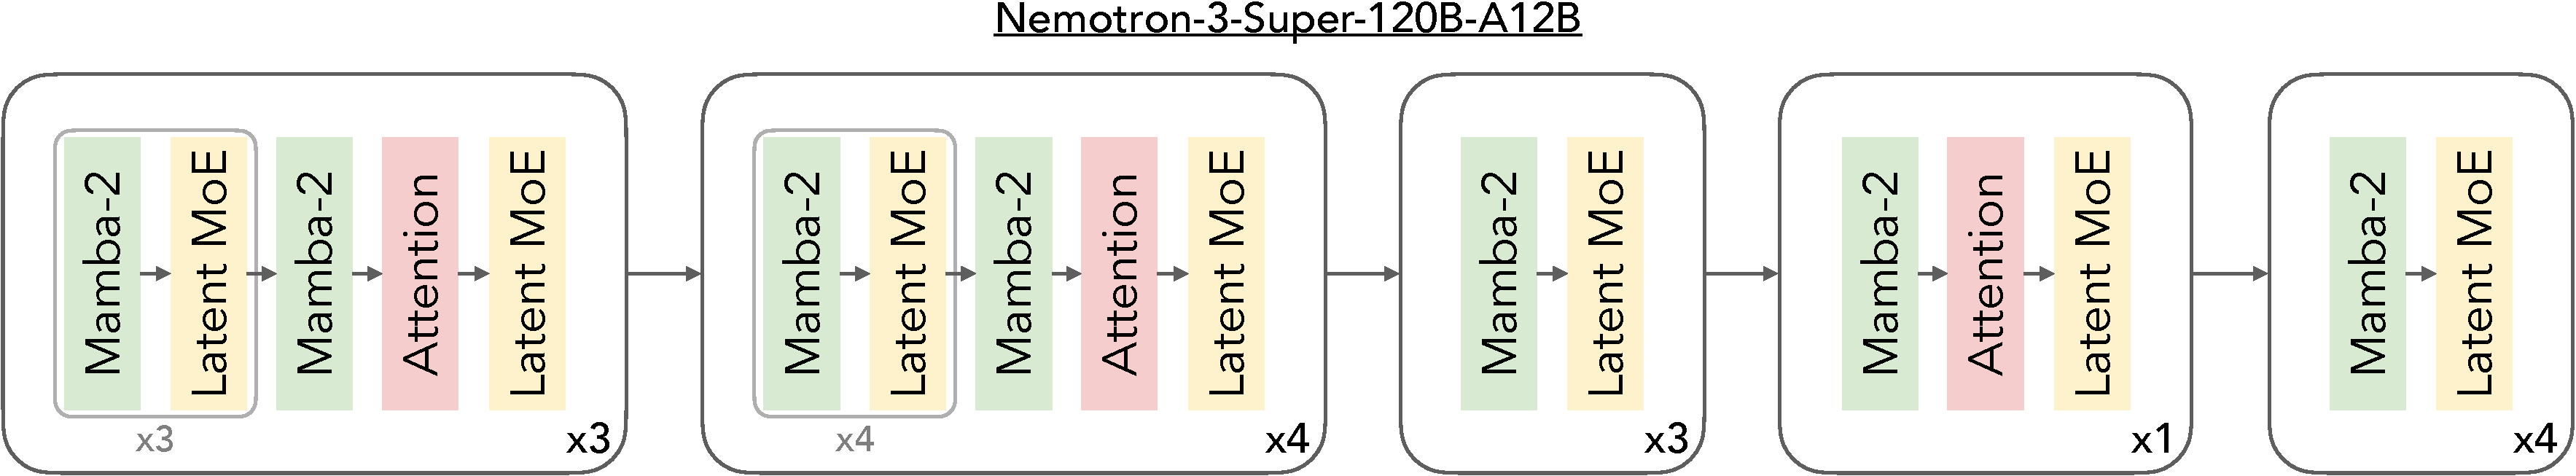
\includegraphics[width=\linewidth]{n3s-fig02-layer-pattern.pdf}
  \caption[Nemotron 3 Super layer pattern]{\NS\ layer pattern: Mamba-2 blocks
  paired with LatentMoE layers, with a few attention layers at intervals.
  \source{NVIDIA (2026)~\cite{nvidia2026super}, Fig.~2}}
  \label{fig:layer-pattern}
\end{figure}

Multiplying out the repeat counts in the pattern gives the layer budget in
Table~\ref{tab:layer-count}. Seven of the eight attention layers fall within
the first 71 layers, and the final eight layers contain none.

\begin{table}[!htbp]
\centering
\small
\caption[Layer budget of Nemotron 3 Super]{Layer budget of \NS, counted by the
author from the published layer pattern}
\label{tab:layer-count}
\begin{tabular}{@{}lcccc@{}}
\toprule
\textbf{Group in the pattern} & \textbf{Mamba-2} & \textbf{Attention} & \textbf{LatentMoE} & \textbf{Layers} \\
\midrule
$[\,(\text{M},\text{E})\times 3,\ \text{M},\ \text{A},\ \text{E}\,]\times 3$ & 12 & 3 & 12 & 27 \\
$[\,(\text{M},\text{E})\times 4,\ \text{M},\ \text{A},\ \text{E}\,]\times 4$ & 20 & 4 & 20 & 44 \\
$(\text{M},\text{E})\times 3$ & 3 & 0 & 3 & 6 \\
$(\text{M},\ \text{A},\ \text{E})\times 1$ & 1 & 1 & 1 & 3 \\
$(\text{M},\text{E})\times 4$ & 4 & 0 & 4 & 8 \\
\midrule
\textbf{Total} & \textbf{40} & \textbf{8} & \textbf{40} & \textbf{88} \\
\bottomrule
\multicolumn{5}{@{}l}{\footnotesize M = Mamba-2 block, A = attention block, E = LatentMoE layer.}
\end{tabular}
\end{table}

The layout is a division of labour. The Mamba-2 blocks do the heavy lifting in
linear time with a constant-size state. The few attention layers act as global
\emph{anchors} where every token can reach every other token, so information
that the Mamba state compressed away can still be retrieved exactly. The
attention layers use GQA with 32 query heads and only 2 KV heads; there are no
positional embeddings, and RMSNorm is used for normalisation.

The saving is large. By the author's estimate, 8 attention layers with 2 KV
heads of dimension 128 store $8 \times 2 \times 2 \times 128 = 4096$ numbers
per token, about 4\,GB at one million tokens in 8-bit precision; using
attention in place of all 40 Mamba blocks too would make it six times larger.
The 40 Mamba-2 states together hold about 42 million numbers---a few tens of
megabytes---regardless of context length.

\section{LatentMoE}

Each MoE layer has 512 experts, 22 of them active per token. LatentMoE~\cite{elango2026latentmoe}
starts from the observation that existing MoE designs are tuned for accuracy
per FLOP, whereas real deployments are limited by other things. NVIDIA's
analysis gives five principles~\cite{nvidia2026super}:
\begin{enumerate}
  \item In low-latency serving the cost is the \emph{memory bandwidth} to read
        expert weights of size $d \times m$, where $d$ is the hidden dimension
        and $m$ the expert's intermediate dimension.
  \item In distributed serving the cost is all-to-all \emph{routing} of tokens,
        whose volume scales as $d \times K$ for $K$ active experts.
  \item Quality depends on the non-linear budget $K \cdot m$, so $K$ and $m$
        should not be reduced.
  \item $d$ can be reduced only down to a task-dependent effective rank;
        below it, quality collapses.
  \item More experts $N$ and more active experts $K$ improve quality, because
        the number of expert combinations grows exponentially.
\end{enumerate}
Principles 1--3 single out $d$ as the quantity to shrink, principle 4 limits
how far, and principle 5 says how to spend the savings. Each token is projected from dimension $d$
into a smaller latent space of size $\ell$, the routed experts work there, and
the result is projected back (Figure~\ref{fig:latentmoe}):
\begin{equation}
  y = W_{\uparrow} \sum_{i \,\in\, \operatorname{TopK}(g(x),\,K')}
      g_i(x)\, E_i\bigl(W_{\downarrow}\,x\bigr) \;+\; E_{\text{shared}}(x).
  \label{eq:latentmoe}
\end{equation}
This cuts weight loads and routing traffic by $\alpha = d/\ell$, and the
saving is spent on $\alpha$ times more experts, improving quality at roughly
the same cost.

\begin{figure}[!htbp]
  \centering
  \begin{subfigure}[t]{0.42\linewidth}
    \centering
    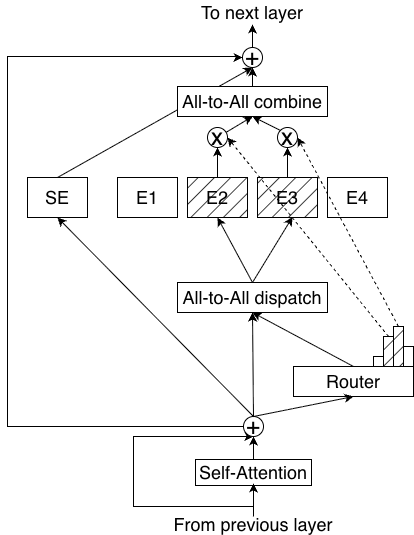
\includegraphics[width=\linewidth]{n3s-fig03a-standard-moe.png}
    \caption{Standard MoE}
  \end{subfigure}\hspace{0.06\linewidth}
  \begin{subfigure}[t]{0.42\linewidth}
    \centering
    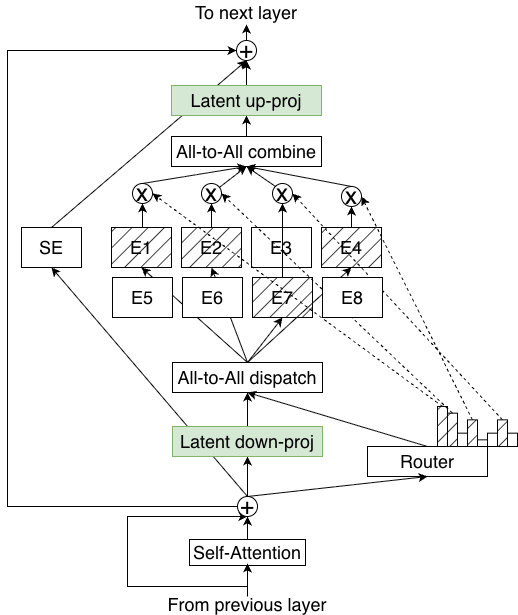
\includegraphics[width=\linewidth]{n3s-fig03b-latent-moe.png}
    \caption{LatentMoE}
  \end{subfigure}
  \caption[Standard MoE compared with LatentMoE]{Standard MoE compared with
  LatentMoE, where tokens are projected into a smaller latent dimension $\ell$
  for routing and expert computation. \source{NVIDIA
  (2026)~\cite{nvidia2026super}, Fig.~3}}
  \label{fig:latentmoe}
\end{figure}

In \NS, $d = 4096$ and $\ell = 1024$, so $\alpha = 4$. By the author's
estimate, the routed experts hold about 113 of the 120.6 billion parameters,
of which only $22/512 \approx 4.3\%$ are used per token---the reason the
active size is about a tenth of the total. On a 95B model with the same
setting, LatentMoE matched or improved on the baseline's validation loss
(Figure~\ref{fig:latentmoe-loss}).

\begin{figure}[!htbp]
  \centering
  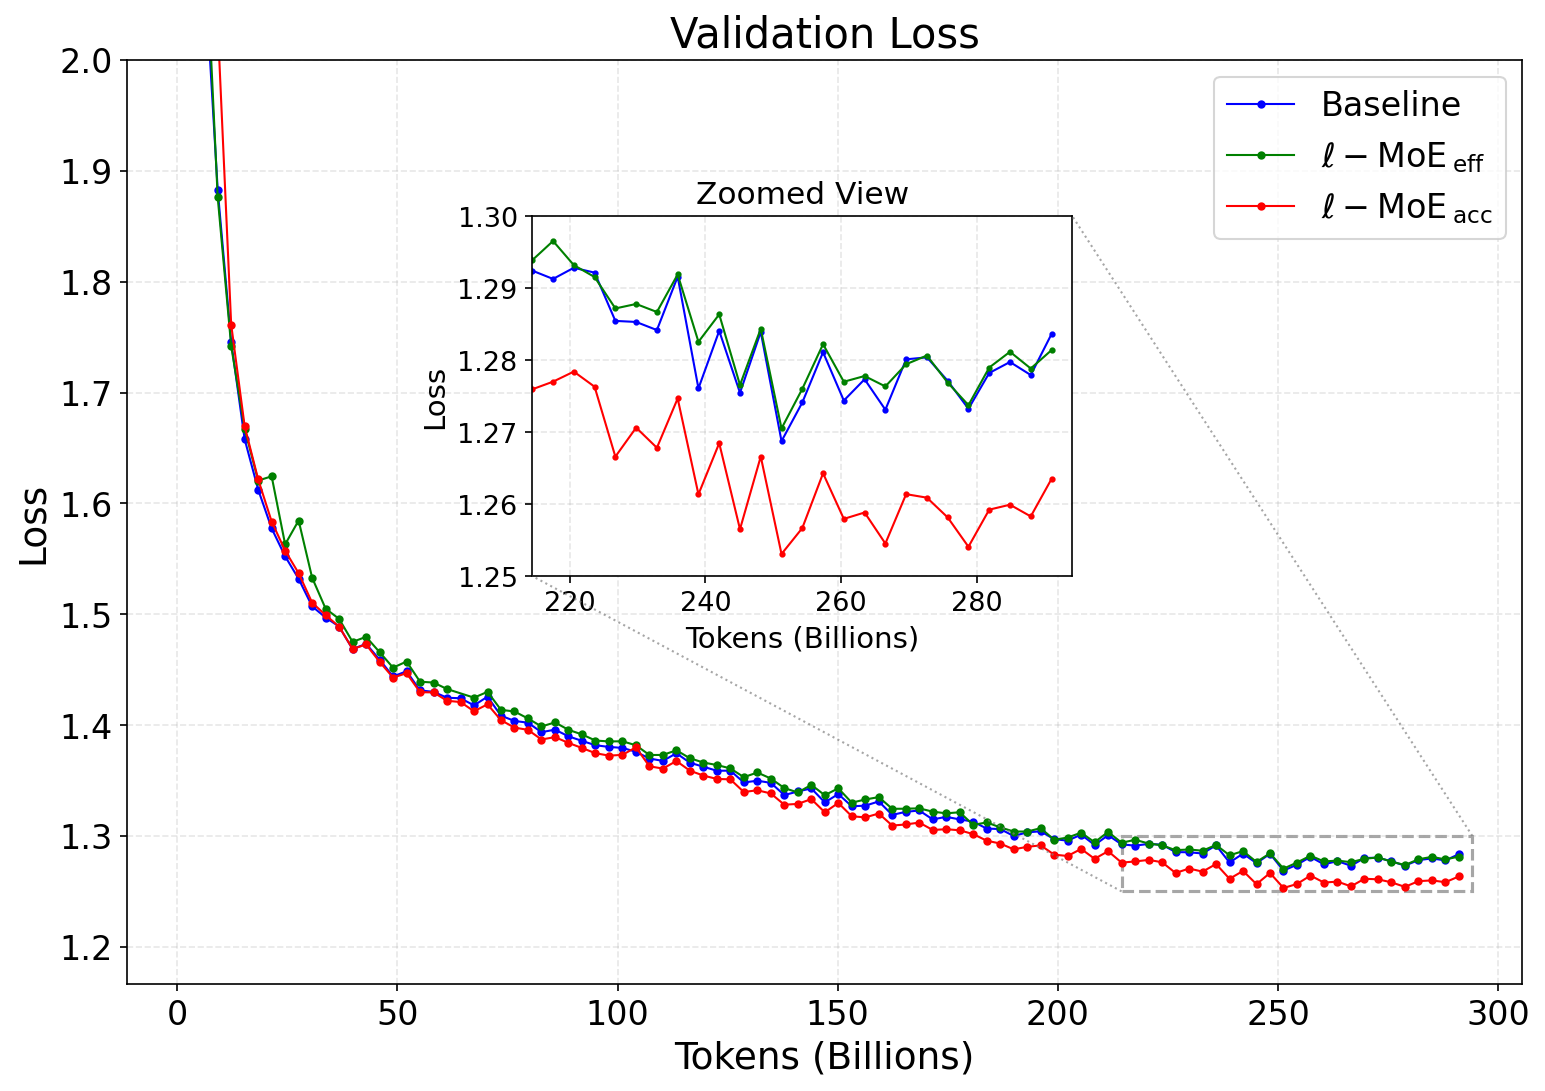
\includegraphics[width=0.6\linewidth]{latentmoe-fig06-95b-val-loss.png}
  \caption[Validation loss of LatentMoE variants on a 95B model]{Validation
  loss of a 95B baseline MoE and two LatentMoE configurations. \source{Elango
  et al.\ (2026)~\cite{elango2026latentmoe}, Fig.~6}}
  \label{fig:latentmoe-loss}
\end{figure}

\section{Multi-Token Prediction}

\NS\ adds an MTP objective~\cite{gloeckle2024mtp,deepseek2024v3}: auxiliary
heads also predict tokens further ahead, and the model is trained on
$\mathcal{L} = \mathcal{L}_{\text{next}} + 0.3\,\mathcal{L}_{\text{MTP}}$,
which improves validation loss and accuracy.

MTP also speeds up generation through speculative
decoding~\cite{leviathan2022speculative,chen2023speculative}: a cheap draft
proposes several tokens, the full model checks them in one pass, and the
agreeing ones are accepted (Figure~\ref{fig:specdec}). The output still
follows the full model's distribution. In \NS\ the MTP heads are the draft
model, so no separate network is needed and the extra computation is small.

Standard MTP uses independent heads, each trained for one fixed offset, which
limits a draft to as many tokens as there are heads. Reusing one head
repeatedly works poorly, because a head trained on ground-truth hidden states
is suddenly fed its own predictions. \NS\ instead \emph{shares the weights} of
its two MTP layers during training, giving a single head exposed to several
offsets. It is more robust to its own outputs, so it can be applied
recursively to draft longer sequences without adding parameters.

\begin{figure}[!htbp]
  \centering
  % Speculative decoding loop with MTP heads as the built-in draft model
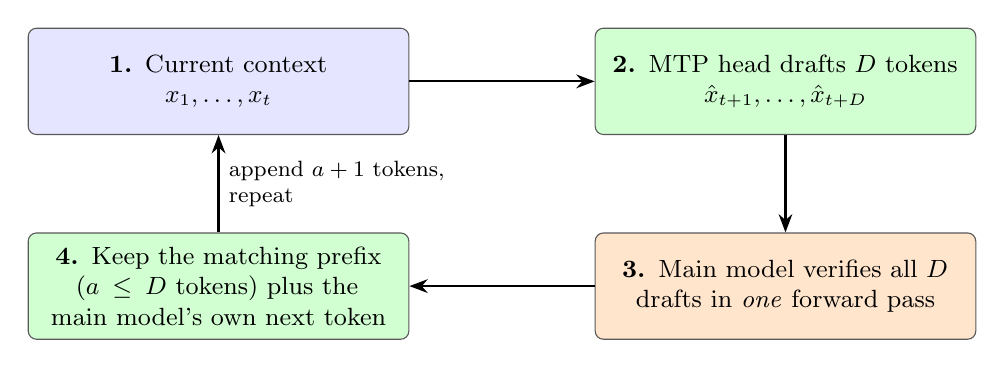
\begin{tikzpicture}[
  font=\small, >={Stealth},
  stp/.style={rectangle, rounded corners=3pt, draw=gray!70!black, fill=blue!10,
              minimum height=1.35cm, text width=4.6cm, align=center}]
\node[stp] (ctx) at (0,0) {\textbf{1.} Current context\\$x_1,\dots,x_t$};
\node[stp, fill=green!18] (draft) at (7.2,0)
  {\textbf{2.} MTP head drafts $D$ tokens\\$\hat{x}_{t+1},\dots,\hat{x}_{t+D}$};
\node[stp, fill=orange!20] (verify) at (7.2,-2.6)
  {\textbf{3.} Main model verifies all $D$ drafts in \emph{one} forward pass};
\node[stp, fill=green!18] (keep) at (0,-2.6)
  {\textbf{4.} Keep the matching prefix ($a \le D$ tokens) plus the main model's own next token};
\draw[->, thick] (ctx) -- (draft);
\draw[->, thick] (draft) -- (verify);
\draw[->, thick] (verify) -- (keep);
\draw[->, thick] (keep) -- node[right, font=\footnotesize, align=left] {append $a+1$ tokens,\\repeat} (ctx);
\end{tikzpicture}

  \caption[Speculative decoding loop using MTP heads]{The speculative decoding
  loop, with the MTP head as the built-in draft model (drawn by the author).}
  \label{fig:specdec}
\end{figure}

On SPEED-Bench with a draft length of 7, \NS\ accepts on average 3.45 tokens
per verification step, more than DeepSeek-R1 (2.70) and Qwen3-Next (3.33), and
leads in eight of eleven categories (Table~\ref{tab:mtp}). Deeper drafts move
the throughput--latency curve outwards (Figure~\ref{fig:mtp-acceptance}).

\begin{table}[!htbp]
\centering
\small
\caption[MTP average acceptance lengths on SPEED-Bench]{MTP average acceptance
lengths on SPEED-Bench, draft length 7 (selected categories
from~\cite{nvidia2026super}, Table~2)}
\label{tab:mtp}
\begin{tabular}{@{}lccc@{}}
\toprule
\textbf{Category} & \textbf{DeepSeek-R1} & \textbf{Qwen3-Next} & \textbf{\NS} \\
\midrule
Coding        & 2.99 & \textbf{4.32} & 3.78 \\
Math          & 2.98 & \textbf{3.89} & 3.73 \\
Multilingual  & 2.83 & 3.97 & \textbf{4.05} \\
RAG           & 2.79 & 3.53 & \textbf{3.78} \\
Reasoning     & 2.80 & 3.47 & \textbf{3.59} \\
Summarization & 2.59 & 3.06 & \textbf{3.48} \\
\midrule
\textbf{Average (all 11)} & 2.70 & 3.33 & \textbf{3.45} \\
\bottomrule
\end{tabular}
\end{table}

\begin{figure}[!htbp]
  \centering
  \begin{subfigure}[b]{0.46\linewidth}
    \centering
    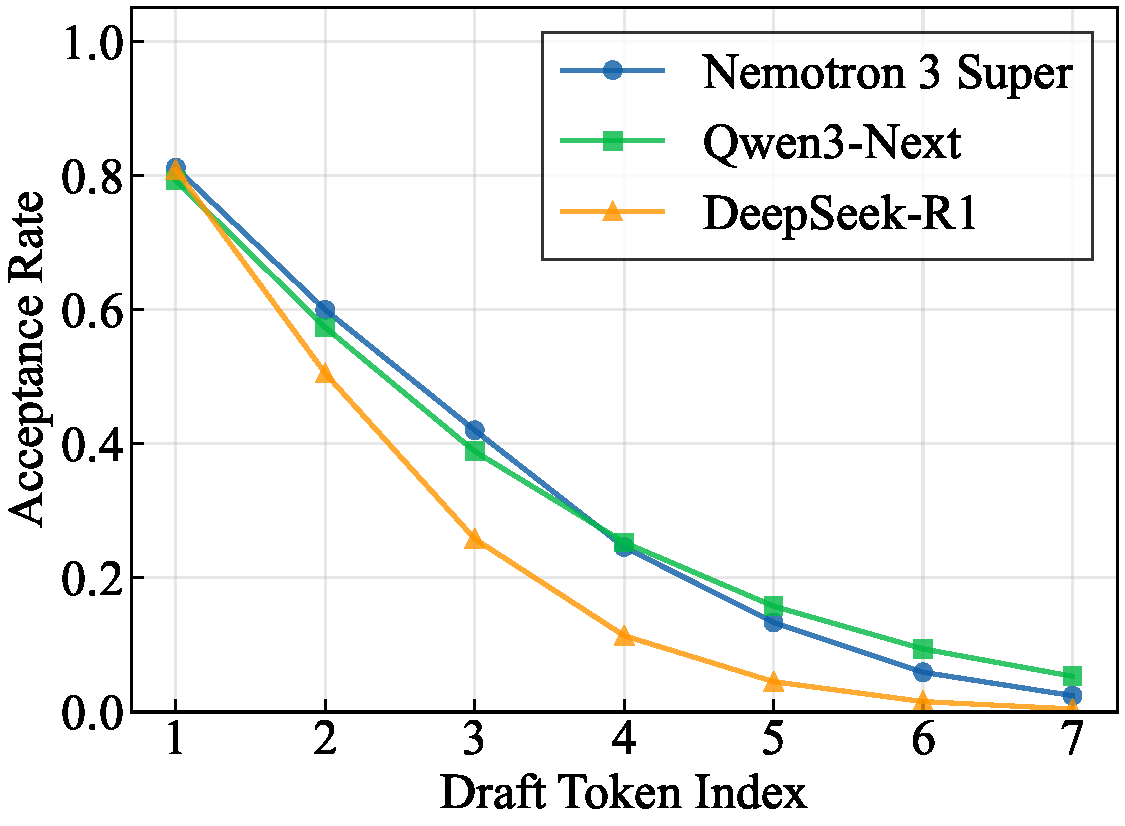
\includegraphics[width=\linewidth]{n3s-fig04-mtp-acceptance.pdf}
    \caption{Acceptance rate by draft index.}
  \end{subfigure}\hfill
  \begin{subfigure}[b]{0.44\linewidth}
    \centering
    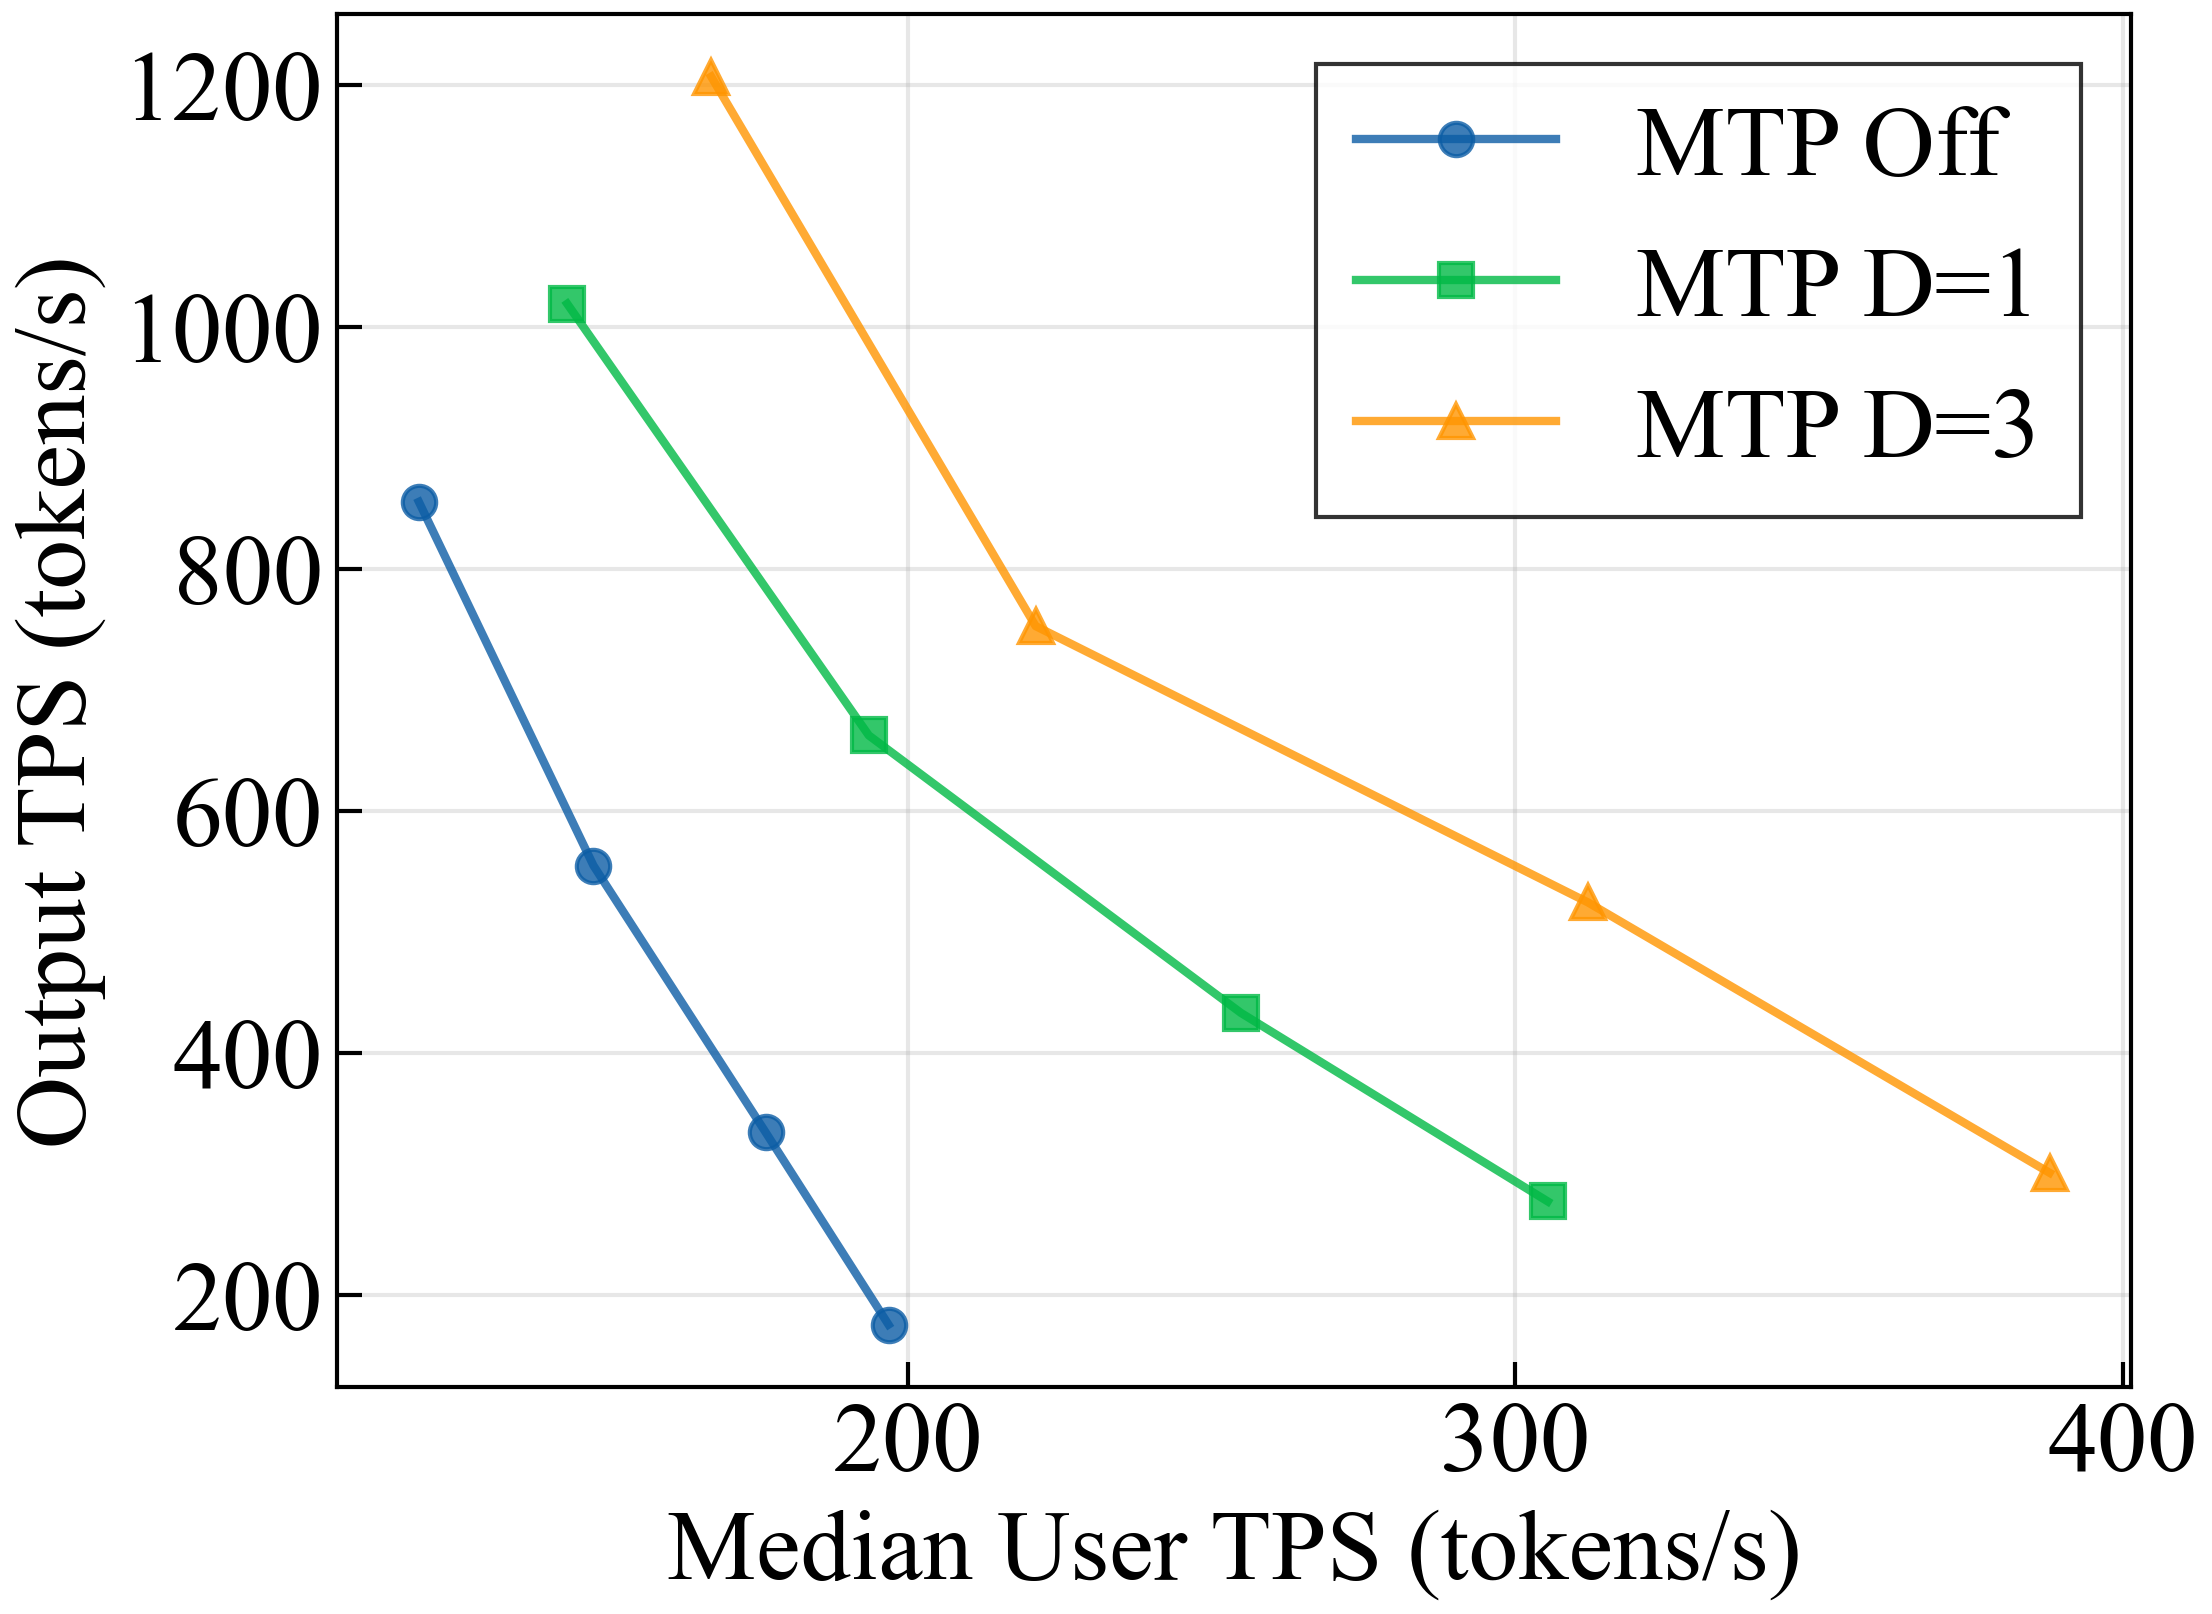
\includegraphics[width=\linewidth]{n3s-fig05-mtp-throughput.png}
    \caption{Throughput with MTP off and draft lengths 1 and 3.}
  \end{subfigure}
  \caption[MTP acceptance rate and serving throughput]{MTP acceptance on
  SPEED-Bench and its effect on serving throughput (NVFP4, B300 GPU).
  \source{NVIDIA (2026)~\cite{nvidia2026super}, Figs.~4 and~5}}
  \label{fig:mtp-acceptance}
\end{figure}

\section{Summary of the Architecture}

\NS\ arranges 88 layers so that 40 Mamba-2 blocks carry most of the sequence
processing, 8 GQA attention layers act as global anchors for exact retrieval,
and 40 LatentMoE layers provide capacity. LatentMoE compresses each token from
4096 to 1024 dimensions before routing, which cuts weight traffic and
communication fourfold and pays for 512 experts with 22 active per token. Two
shared-weight MTP layers improve training and act as a built-in draft model,
accepting on average 3.45 tokens per verification step. Together these choices
give a model with the capacity of 120 billion parameters, the per-token cost of
about 12 billion, and a KV cache only one sixth the size it would otherwise be.

\chapter{Training}
\label{ch:training}

\NS\ is pretrained on 25 trillion tokens in NVFP4 precision, extended to a
one-million-token context, fine-tuned on more than 7 million samples, trained
with reinforcement learning, and finally has its MTP heads retrained.

\section{NVFP4 Pretraining}

NVFP4~\cite{nvidia2025nvfp4} is a 4-bit format natively accelerated on NVIDIA
Blackwell GPUs. Each value is a 4-bit E2M1 number; blocks of 16 values share
an 8-bit (E4M3) scale, and a second FP32 scale is applied per tensor
(Figure~\ref{fig:nvfp4-format}), about 4.5 bits per value. Its smaller blocks
make it more accurate than MXFP4.

\begin{figure}[!htbp]
  \centering
  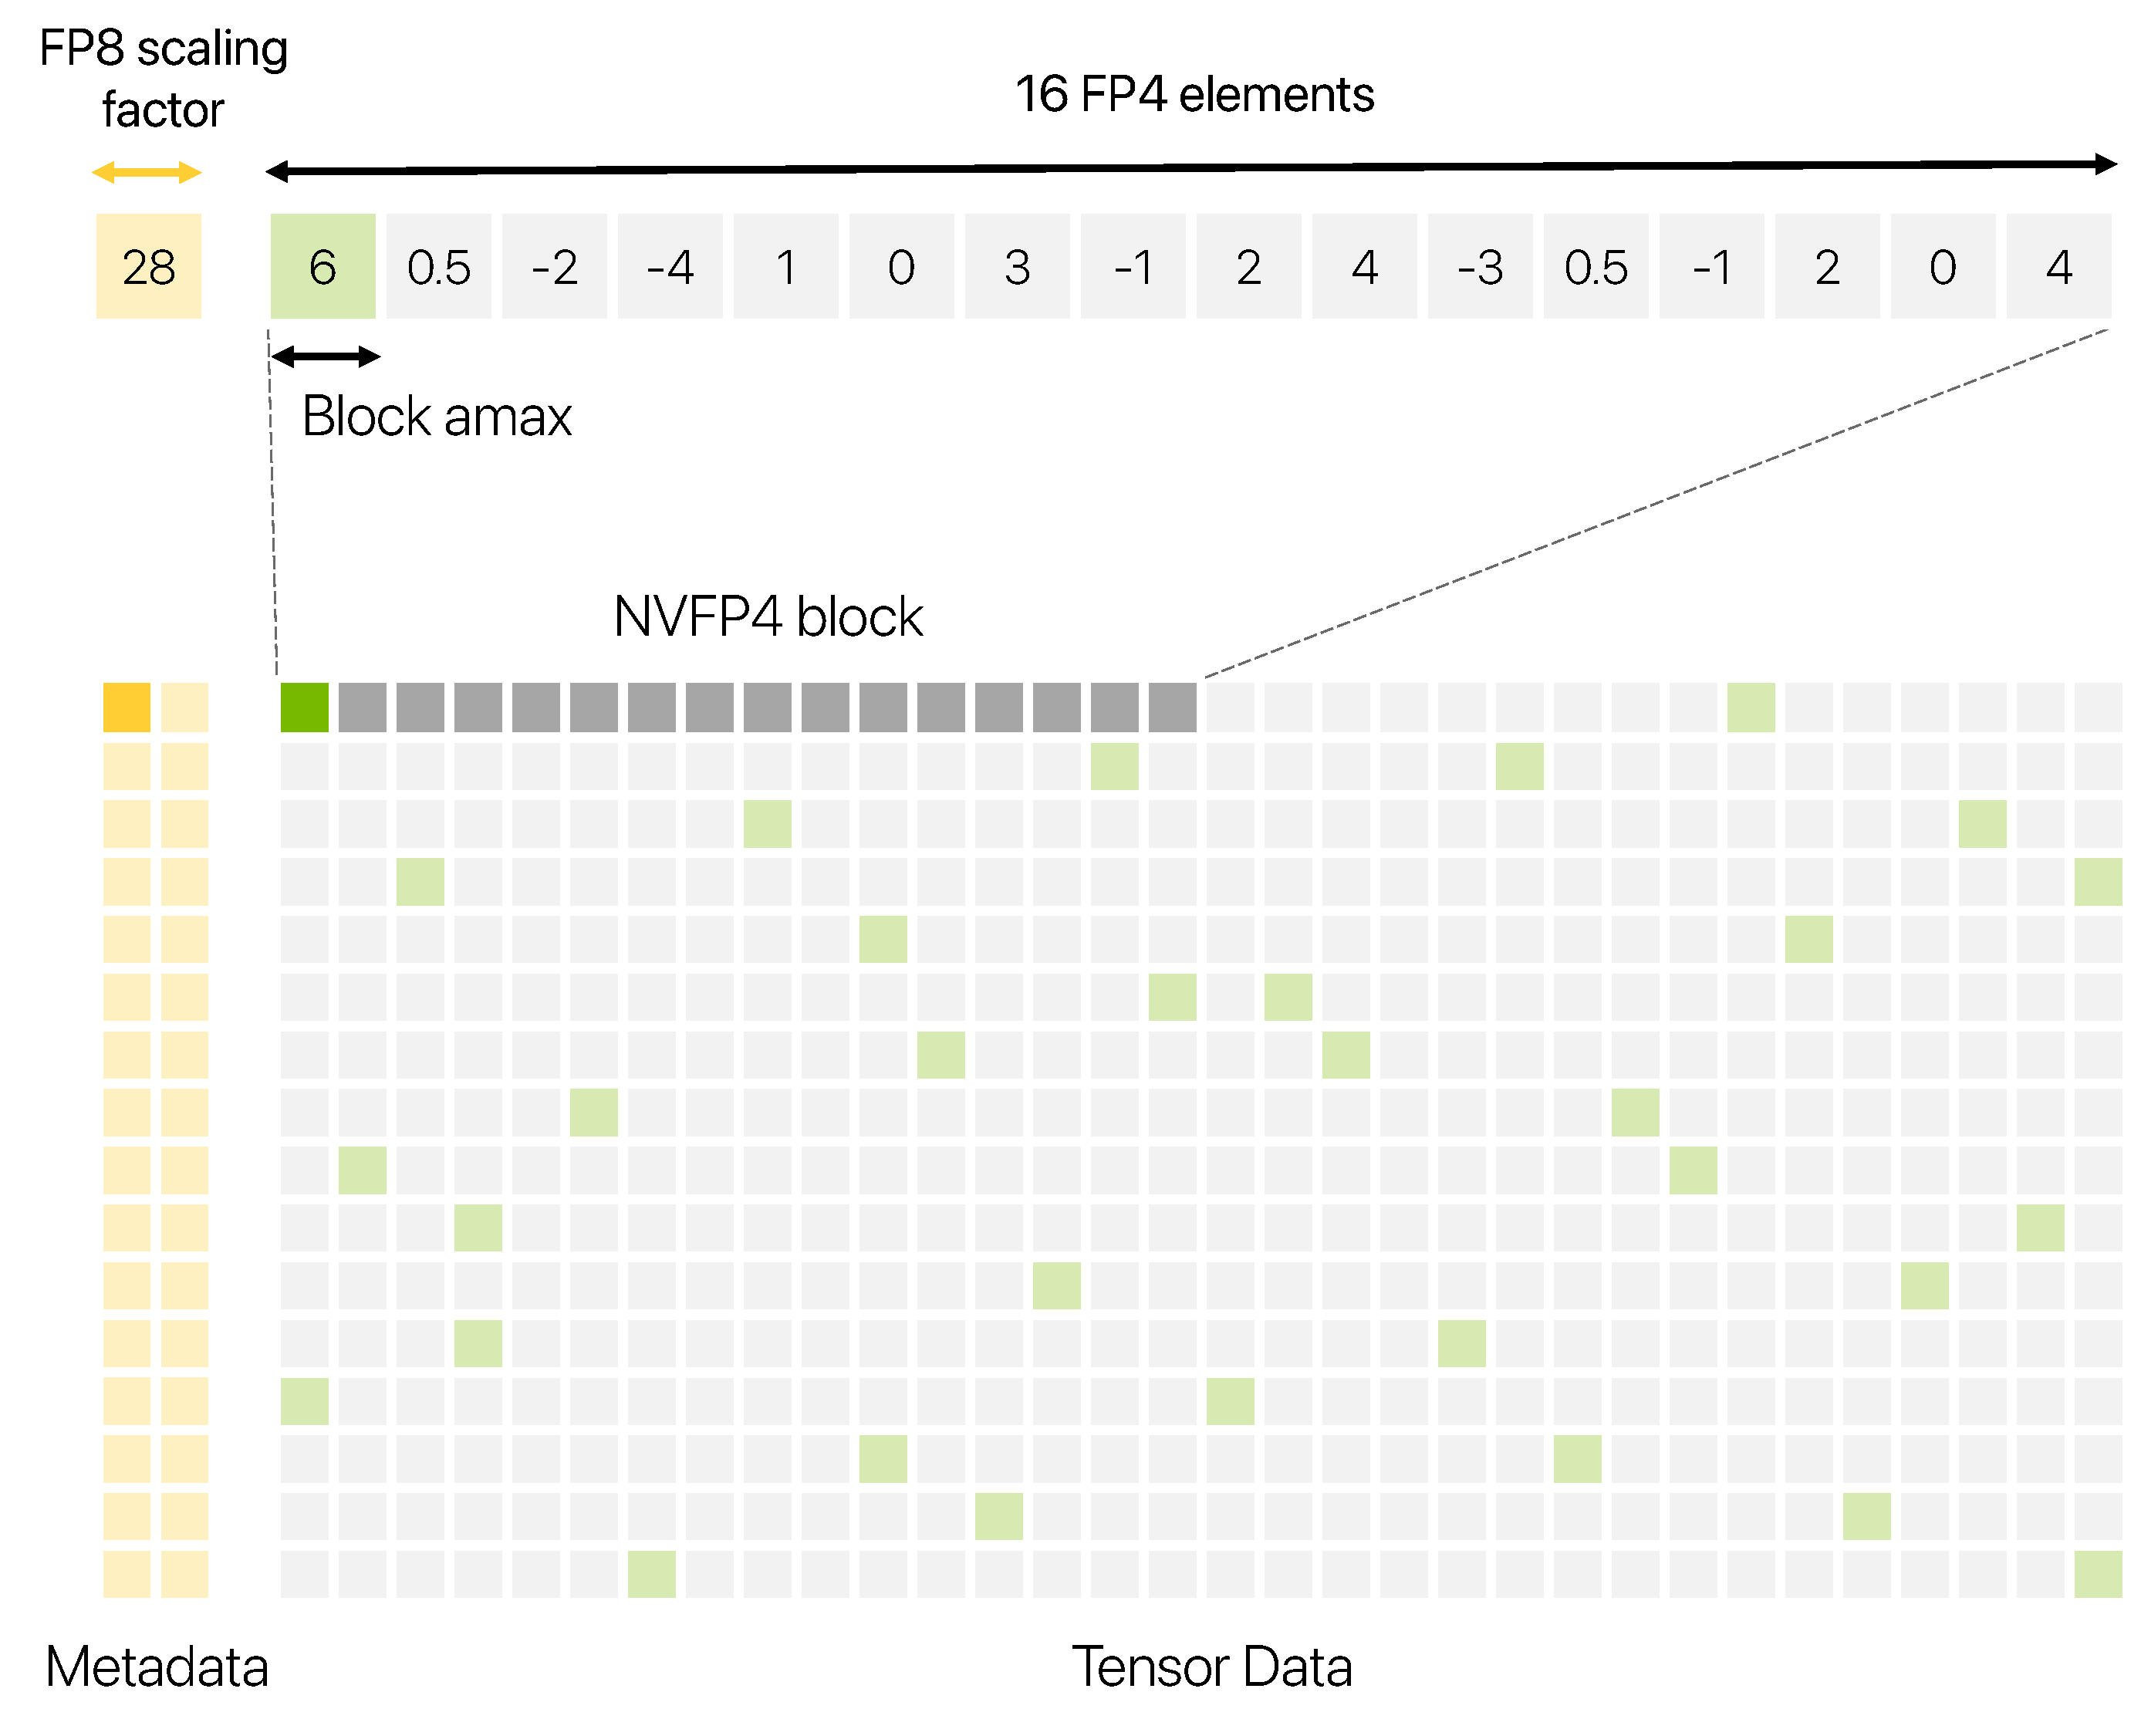
\includegraphics[width=0.48\linewidth]{nvfp4-fig01-format.pdf}
  \caption[A matrix stored in NVFP4 format]{A matrix stored in NVFP4: each
  block holds sixteen FP4 elements and one FP8 scale. \source{NVIDIA
  (2025)~\cite{nvidia2025nvfp4}, Fig.~1}}
  \label{fig:nvfp4-format}
\end{figure}

Simply rounding everything to 4 bits makes training diverge. The recipe uses
two-dimensional block scaling for weights, Random Hadamard Transforms to spread
outliers, stochastic rounding of gradients, and keeps a few sensitive layers in
higher precision (Table~\ref{tab:precision-train}). On a 12B model this kept
the loss close to FP8 over 10T tokens (Figure~\ref{fig:nvfp4-loss}).

\begin{figure}[!htbp]
  \centering
  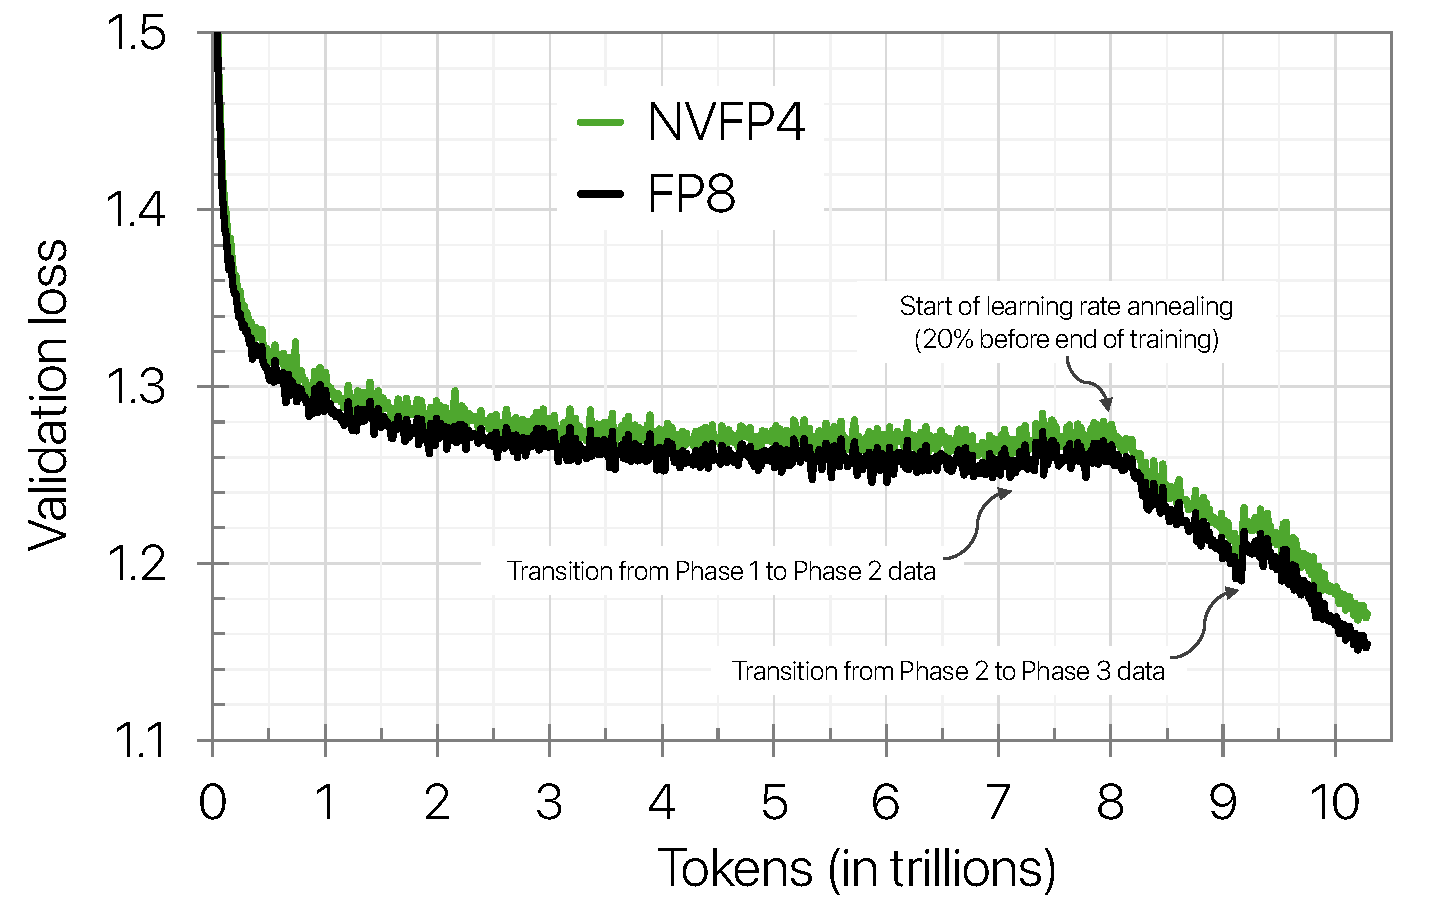
\includegraphics[width=0.6\linewidth]{nvfp4-fig02-val-loss.pdf}
  \caption[Validation loss of NVFP4 versus FP8 pretraining]{Validation loss of
  NVFP4 and FP8 pretraining for a 12B model. \source{NVIDIA
  (2025)~\cite{nvidia2025nvfp4}, Fig.~2}}
  \label{fig:nvfp4-loss}
\end{figure}

\begin{table}[!htbp]
\centering
\small
\caption[Training precision by layer type]{Training precision by layer type
(from~\cite{nvidia2026super}, Table~3)}
\label{tab:precision-train}
\begin{tabularx}{\linewidth}{@{}P{4.6cm}cL@{}}
\toprule
\textbf{Layer type} & \textbf{Format} & \textbf{Rationale} \\
\midrule
All linear layers unless noted & NVFP4 & Default \\
Final 15\% of the network & BF16 & Training stability at scale \\
Latent projections, embeddings & BF16 & Negligible effect on step time \\
MTP and attention layers & BF16 & Preserve fidelity of these few layers \\
Mamba output projection & MXFP8 & Avoids underflow seen with NVFP4 \\
\bottomrule
\end{tabularx}
\end{table}

Training was stable over all 25T tokens. Zero-valued weight gradients grew to
7\% of parameters; a controlled test on \NN\ showed NVFP4 produces about three
times more than BF16 because 4-bit quantization underflows tiny gradients
(Figure~\ref{fig:nvfp4-zeros}). Switching to MXFP8 at 19T tokens gave no
lasting downstream gain (Figure~\ref{fig:nvfp4-healing}), so NVFP4 was kept
throughout.

\begin{figure}[!htbp]
  \centering
  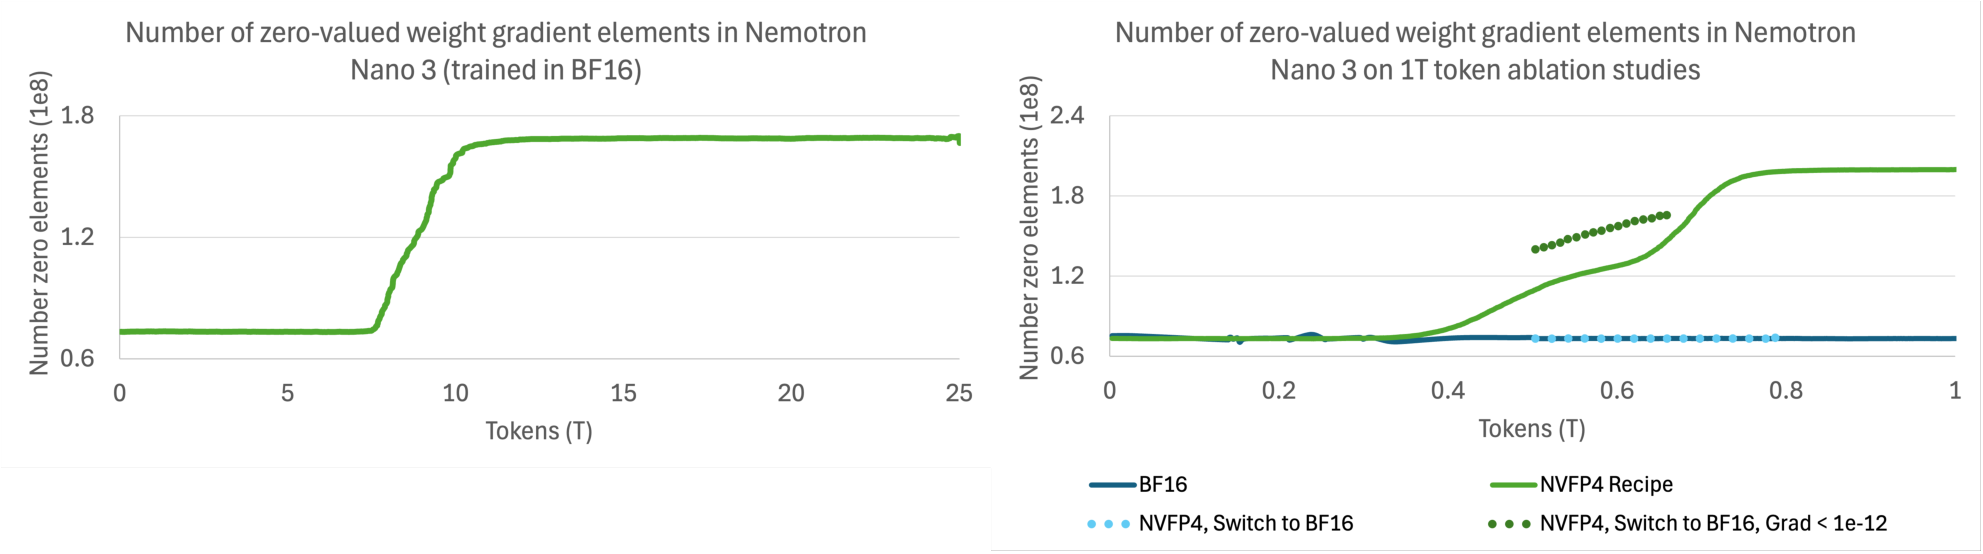
\includegraphics[width=0.92\linewidth]{n3s-fig07-nvfp4-zero-grads.pdf}
  \caption[Zero-valued weight gradients under NVFP4 and BF16 training]{Zero-valued
  weight-gradient elements on \NN\ under BF16 and NVFP4. \source{NVIDIA
  (2026)~\cite{nvidia2026super}, Fig.~7}}
  \label{fig:nvfp4-zeros}
\end{figure}

\begin{figure}[!htbp]
  \centering
  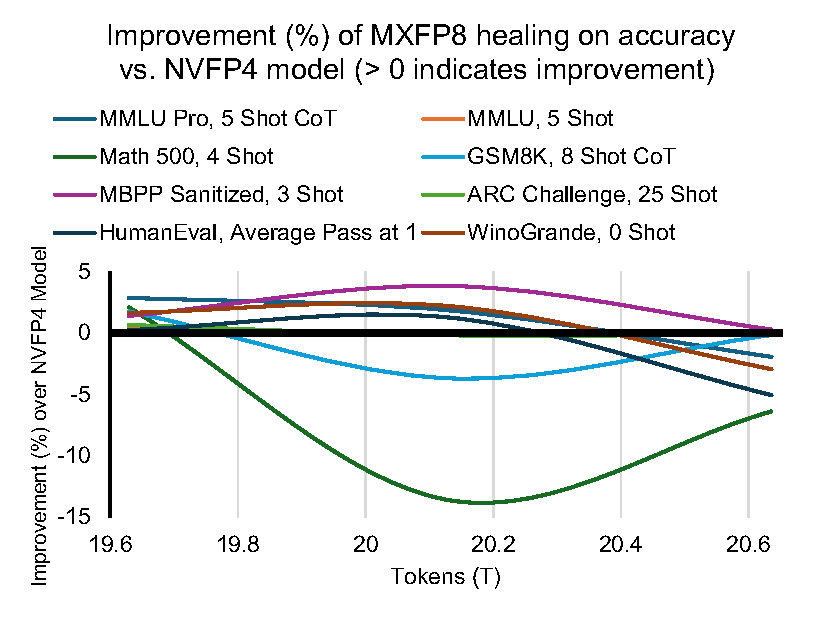
\includegraphics[width=0.52\linewidth]{n3s-fig09-nvfp4-healing.pdf}
  \caption[Effect of switching from NVFP4 to MXFP8 late in pretraining]{Change
  in downstream accuracy after switching to MXFP8. \source{NVIDIA
  (2026)~\cite{nvidia2026super}, Fig.~9}}
  \label{fig:nvfp4-healing}
\end{figure}

\section{Pretraining Data and Optimisation}

The corpus spans 16 categories---web crawl in quality tiers with synthetic
rewrites, mathematics, Wikipedia, code, academic, multilingual and synthetic
instruction data---plus new synthetic sets for code concepts, algorithmic
problems, economics, formal logic and multiple-choice reasoning. A two-phase
curriculum (Figure~\ref{fig:blends}) uses diverse data for the first 20T tokens
and shifts to high-quality sources for the last 5T.

\begin{figure}[!htbp]
  \centering
  \begin{subfigure}[b]{0.44\linewidth}
    \centering
    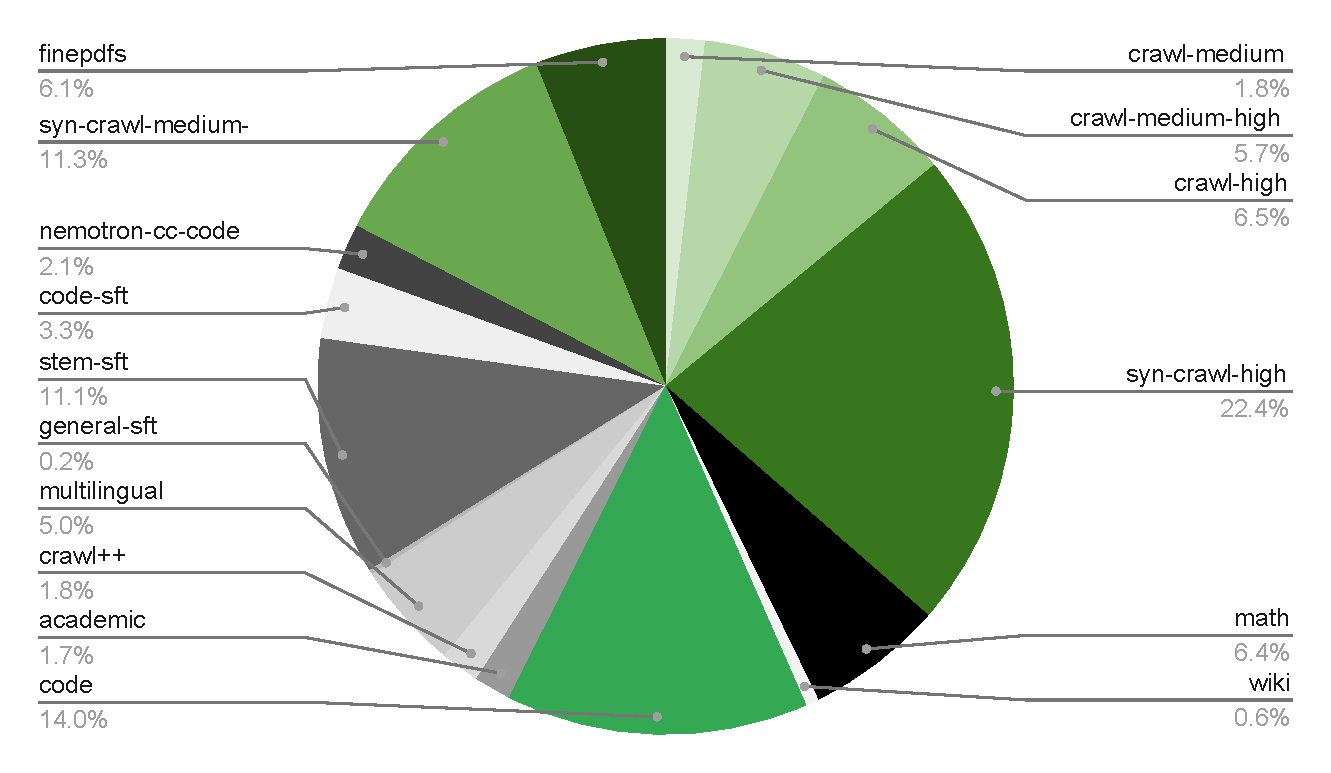
\includegraphics[width=\linewidth]{n3s-fig10a-phase1-blend.pdf}
    \caption{Phase 1}
  \end{subfigure}\hfill
  \begin{subfigure}[b]{0.44\linewidth}
    \centering
    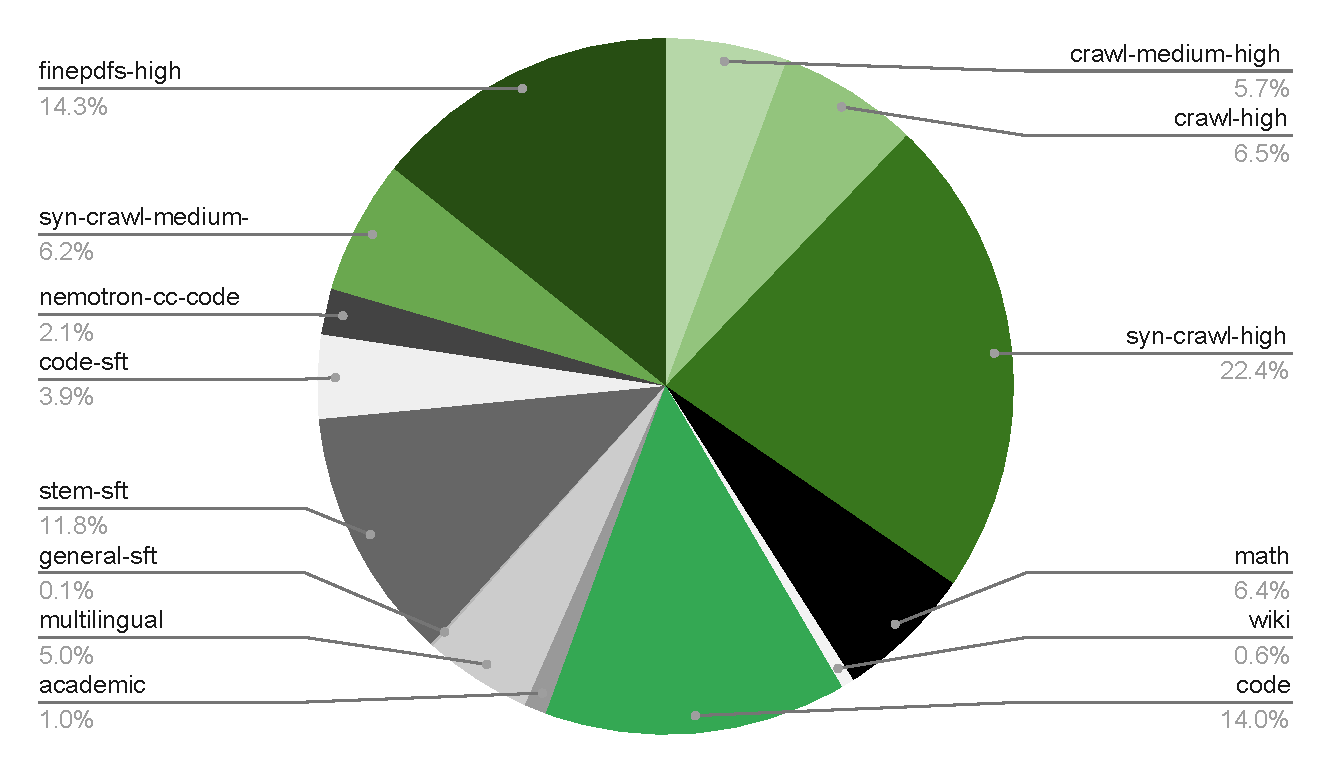
\includegraphics[width=\linewidth]{n3s-fig10b-phase2-blend.pdf}
    \caption{Phase 2}
  \end{subfigure}
  \caption[Data mixtures for the two pretraining phases]{Data mixtures for the
  two pretraining phases. \source{NVIDIA (2026)~\cite{nvidia2026super},
  Fig.~10}}
  \label{fig:blends}
\end{figure}

Training uses AdamW with a Warmup--Stable--Decay schedule (peak learning rate
$4.5 \times 10^{-4}$), 8192-token sequences and about 25M tokens per step.
Instead of separate decay runs to track progress, recent checkpoints were
\emph{merged} by weighted averaging; merges scored 2--4 points higher than raw
checkpoints during the stable phase (Figure~\ref{fig:merge}), saving an
estimated 16\% of pretraining compute.

\begin{figure}[!htbp]
  \centering
  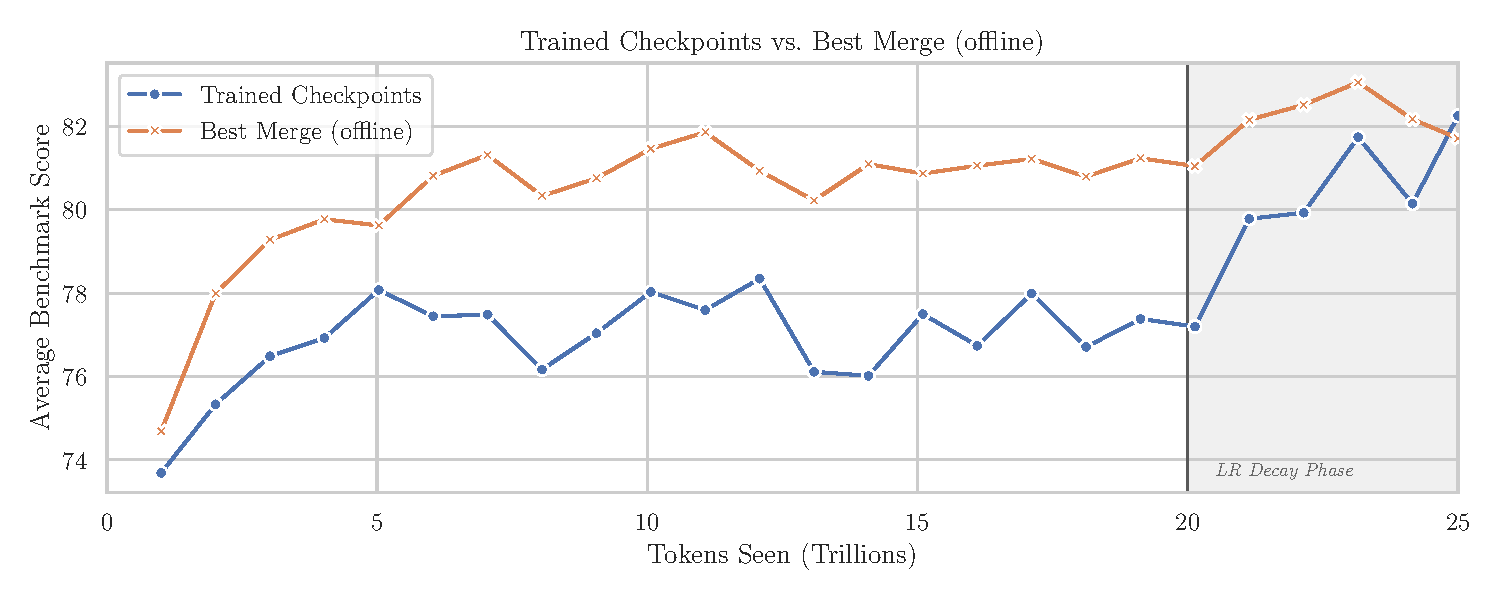
\includegraphics[width=0.85\linewidth]{n3s-fig11-checkpoint-merge.pdf}
  \caption[Trained checkpoints versus merged checkpoints during pretraining]{Average
  accuracy over 12 benchmarks for trained and merged checkpoints.
  \source{NVIDIA (2026)~\cite{nvidia2026super}, Fig.~11}}
  \label{fig:merge}
\end{figure}

A final long-context phase continues at a constant learning rate on 20\%
long-document question-answering data and 80\% Phase~2 data: 34B tokens at a
context of 1,048,576 tokens, then 17B tokens alternating 1M and 4k sequences to
remove a small regression on mathematics. Million-token sequences need 64-way
context parallelism and 64-way expert parallelism on GB200 GPUs; this is
practical because 80 of the 88 layers have no quadratic cost.

\section{Supervised Fine-Tuning}

Post-training follows Figure~\ref{fig:posttraining}. SFT uses more than 7
million samples. A single-stage SFT degraded tasks with long inputs and short
outputs, so two stages with different loss normalisation are used. For a batch
$\mathcal{B}$ of conversations $c$, with output positions $\mathcal{O}_c$ and
token loss $\ell_t$, Stage~1 averages over all output tokens and Stage~2 first
within each conversation:
\begin{equation}
  \mathcal{L}_{\text{tok}} =
  \frac{\sum_{c \in \mathcal{B}} \sum_{t \in \mathcal{O}_c} \ell_t}
       {\sum_{c \in \mathcal{B}} |\mathcal{O}_c|},
  \qquad
  \mathcal{L}_{\text{samp}} =
  \frac{1}{|\mathcal{B}|} \sum_{c \in \mathcal{B}}
  \frac{1}{|\mathcal{O}_c|} \sum_{t \in \mathcal{O}_c} \ell_t .
\end{equation}
Stage~1 gives strong token-level supervision that induces reasoning; Stage~2
stops very long outputs from dominating, restoring long-input, short-output
behaviour. Stage~1 packs sequences up to 256k tokens and Stage~2 up to 512k.
Agentic data---GitHub issues, terminal use, web search, SQL, tool calling and
more---takes a much larger share than for \NN\ (Figure~\ref{fig:sft-blend}).
The model supports reasoning off, regular and a new low-effort mode.

\begin{figure}[!htbp]
  \centering
  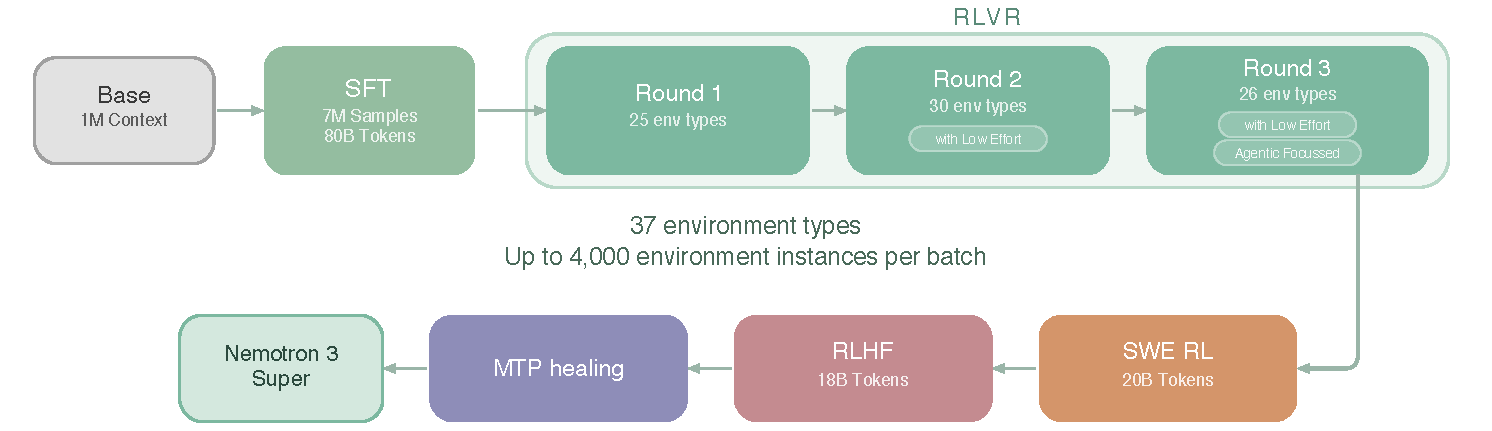
\includegraphics[width=0.92\linewidth]{n3s-fig12-posttraining-stages.pdf}
  \caption[Post-training pipeline of Nemotron 3 Super]{Post-training pipeline:
  SFT, three RL stages and MTP healing. \source{NVIDIA
  (2026)~\cite{nvidia2026super}, Fig.~12}}
  \label{fig:posttraining}
\end{figure}

\begin{figure}[!htbp]
  \centering
  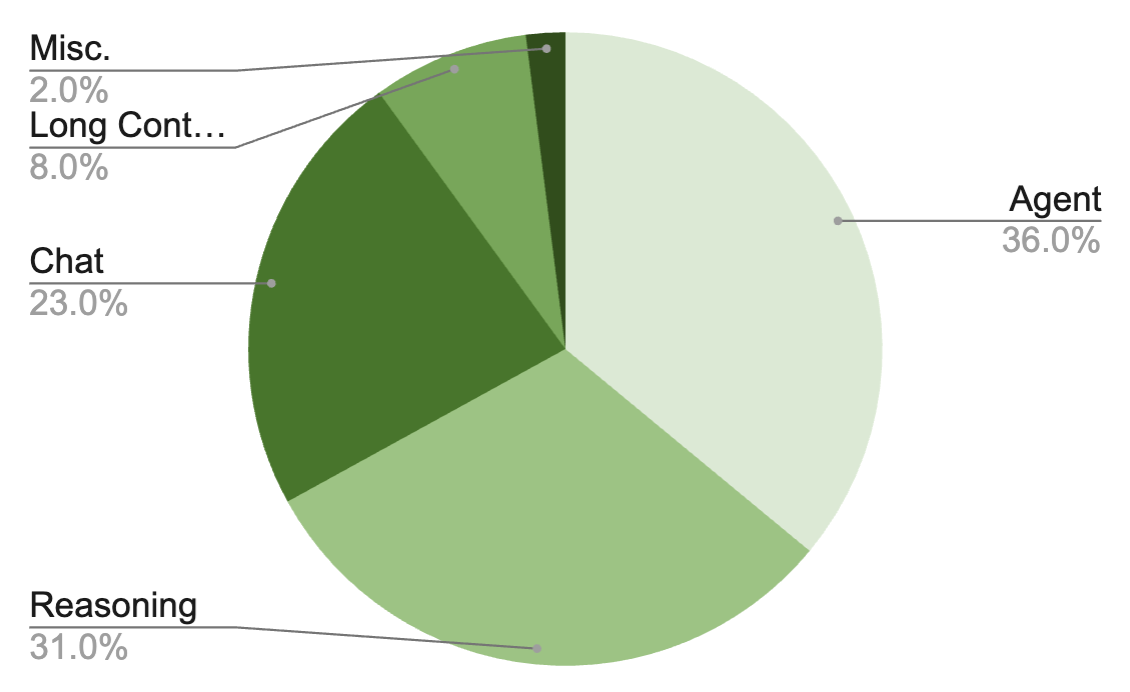
\includegraphics[width=0.52\linewidth]{n3s-fig16-sft-blend.jpg}
  \caption[SFT data blend for Nemotron 3 Super]{SFT data blend for \NS.
  \source{NVIDIA (2026)~\cite{nvidia2026super}, Fig.~16}}
  \label{fig:sft-blend}
\end{figure}

\section{Reinforcement Learning}

\textbf{Stage 1 -- RL from verifiable rewards.} The model is trained jointly
on 21 environments and 37 datasets (mathematics, code, STEM, safety, chat,
long context, agentic tasks) where rewards can be checked automatically.
Training on all at once avoided the regressions seen with single environments.
Easy prompts are filtered and the rest ordered by difficulty, a curriculum
shown to help on \NN\ (Figure~\ref{fig:rl-curriculum}). The algorithm is
asynchronous GRPO: inference workers generate trajectories continuously into a
buffer, full batches go to the trainer, and updated weights are pushed back
with workers never more than one step behind. Each step uses 256 prompts with
16 responses each, with generation length raised from 49K to 64K tokens. For
long-horizon agentic tasks, \emph{PivotRL} reuses expert trajectories and
focuses training on the ``pivot'' turns where the model is uncertain.

\begin{figure}[!htbp]
  \centering
  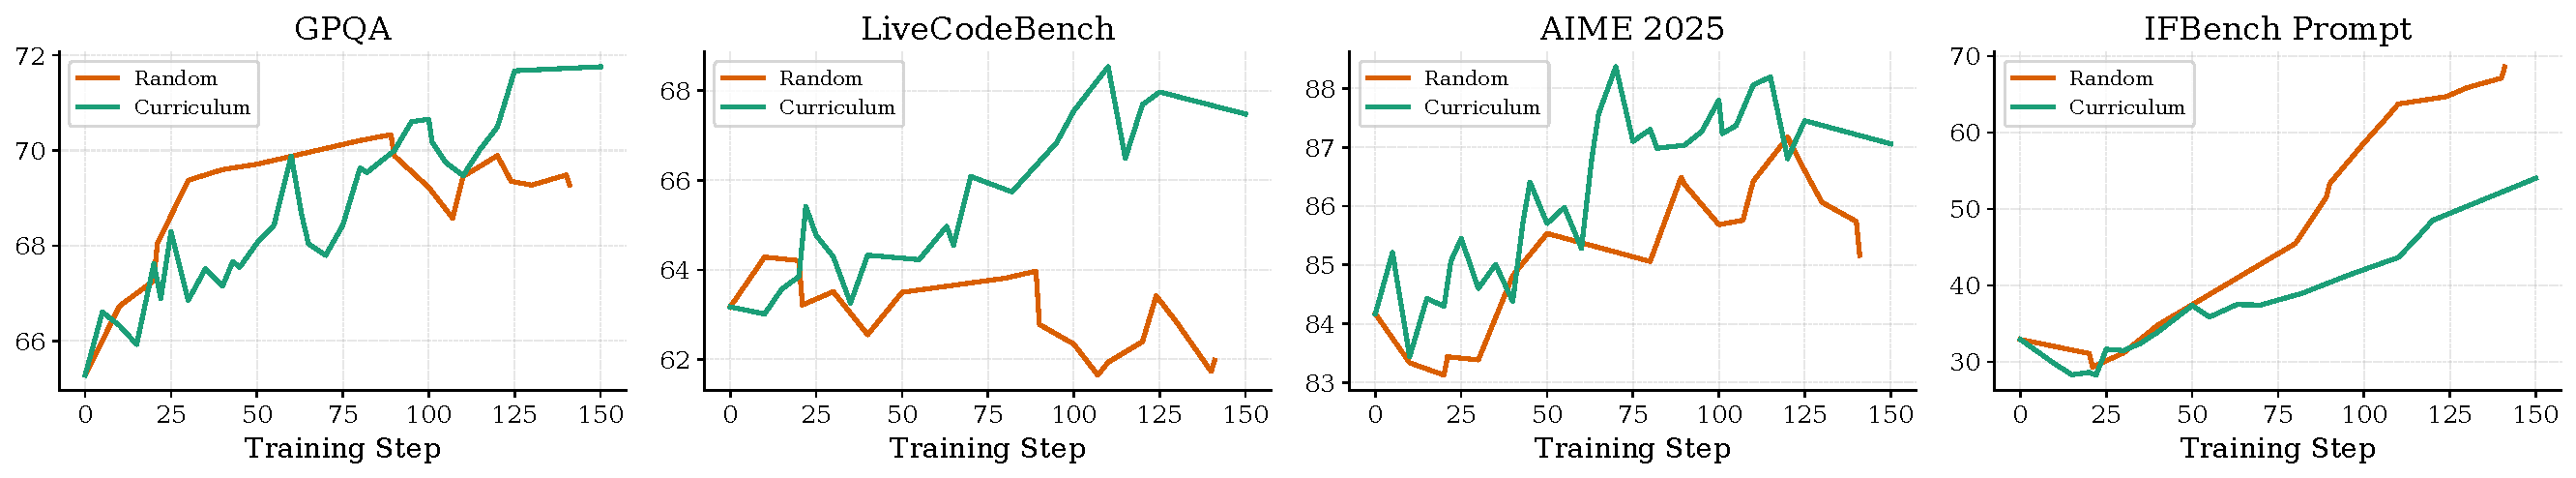
\includegraphics[width=0.85\linewidth]{nano3-fig07-rl-curriculum.pdf}
  \caption[Curriculum sampling versus random sampling in RL]{Curriculum versus
  random sampling during RL on \NN. \source{NVIDIA
  (2025)~\cite{nvidia2025nano3}, Fig.~7}}
  \label{fig:rl-curriculum}
\end{figure}

\textbf{Stage 2 -- Software engineering.} Each rollout runs an agent in a
container to produce a code patch, rewarded by the repository's tests.

\textbf{Stage 3 -- RL from human feedback.} A generative reward model trained
on human preferences improves instruction following and interaction quality.

\textbf{MTP healing.} Finally the network is frozen and only the MTP heads are
retrained on the model's own outputs, restoring their drafting accuracy.

\chapter{Quantization and Deployment}
\label{ch:quant}

After training, the model is compressed so that it runs faster and uses less
memory. NVIDIA applies \emph{post-training quantization} (PTQ) to the weights
and activations of the post-trained BF16 model and releases two deployment
checkpoints: an FP8 checkpoint (8-bit weights and activations) for
Hopper-generation GPUs, and an NVFP4 checkpoint (4-bit weights and
activations) for the newer Blackwell GPUs~\cite{nvidia2026super}.

\section{FP8 Checkpoint}

The FP8 checkpoint was calibrated on 256 samples of 65{,}536 tokens each,
drawn from the SFT data. Quantization is applied to the MoE matrix
multiplications (both routed and shared experts) and to the Mamba linear
layers, where most of the computation is. The KV cache is kept in FP8, and the
Mamba state cache is stored in FP16 rather than FP32 for speed.
Table~\ref{tab:precision-fp8} lists the assignments.

\begin{table}[htbp]
\centering
\small
\caption[Precision settings of the FP8 checkpoint]{Precision settings of the
FP8 checkpoint and of the BF16 baseline (from~\cite{nvidia2026super},
Table~6)}
\label{tab:precision-fp8}
\begin{tabular}{@{}lcc@{}}
\toprule
\textbf{Component} & \textbf{FP8 checkpoint} & \textbf{BF16 baseline} \\
\midrule
Embedding & BF16 & BF16 \\
Attention projections (QKV and output) & BF16 & BF16 \\
KV cache and first attention product & FP8 & FP8 \\
Second attention product & BF16 & BF16 \\
\midrule
MoE experts (routed and shared) & FP8 & BF16 \\
MoE latent projections & BF16 & BF16 \\
Router & FP32 & FP32 \\
\midrule
Mamba linear layers & FP8 & BF16 \\
Mamba SSM cache & FP16 & FP32 \\
Mamba 1-D convolution & BF16 & BF16 \\
\midrule
Output layers & BF16 & BF16 \\
\bottomrule
\end{tabular}
\end{table}

\section{NVFP4 Checkpoint}

FP4 is a more aggressive format than FP8. It is particularly attractive for
prefill-heavy workloads such as coding agents, in which very long inputs are
processed and the linear and MoE matrix multiplications dominate the running
time. NVFP4 for inference uses the same element format as in training: signed
E2M1 values with a scale per block of 16, the block scales being stored in FP8
with a per-tensor FP32 factor.

Naive 4-bit quantization costs accuracy. The final recipe combines three
measures:
\begin{enumerate}
  \item \textbf{MSE-calibrated weight scales.} In the default recipe each
        block scale is set from the largest absolute value in the block.
        Because weights are quantized once, offline, an expensive search can
        be afforded instead, choosing the scale that minimises the mean squared
        error of the block.
  \item \textbf{Max-based activation scales.} Activations must be quantized at
        run time, where a search is impractical, so they keep the simple
        max-based scaling.
  \item \textbf{AutoQuantize.} Sensitive layers are selectively promoted from
        FP4 to FP8 or BF16.
\end{enumerate}

\emph{AutoQuantize}, part of NVIDIA's Model-Optimizer toolkit, selects the
best precision for each layer automatically. It estimates how sensitive each
operation is to quantization, using a second-order approximation of the change
in loss, models the performance cost of each candidate precision, and then
solves a knapsack-style optimisation for the assignment that loses the least
accuracy within a given budget. For \NS\ the candidates were NVFP4, FP8 and
BF16 with an effective budget of 4.75 bits. The outcome
(Table~\ref{tab:precision-fp4}) is a model that is mostly FP4: the routed
experts, which hold the great majority of the parameters, are NVFP4
throughout, while the attention and Mamba projections were assigned FP8 or
BF16.

\begin{table}[htbp]
\centering
\small
\caption[Precision settings of the NVFP4 checkpoint]{Precision settings of the
NVFP4 checkpoint (from~\cite{nvidia2026super}, Table~7)}
\label{tab:precision-fp4}
\begin{tabular}{@{}lcc@{}}
\toprule
\textbf{Component} & \textbf{Searched?} & \textbf{NVFP4 checkpoint} \\
\midrule
Embedding & No & BF16 \\
Attention QKV projection & Yes & BF16 \\
Attention output projection & Yes & FP8 / BF16 \\
KV cache and first attention product & No & FP8 \\
\midrule
Routed (sparse) experts & Yes & NVFP4 \\
Shared expert & Yes & NVFP4 / FP8 / BF16 \\
MoE latent projections & Yes & FP8 / BF16 \\
Router & No & FP32 \\
\midrule
Mamba projections & Yes & FP8 / BF16 \\
Mamba 1-D convolution & No & BF16 \\
Mamba SSM cache & No & FP16 \\
\midrule
Output layers & No & BF16 \\
\bottomrule
\end{tabular}
\end{table}

The whole mixed-precision PTQ process took less than two hours on a single
node with eight B200 GPUs, using 512 calibration samples of 4096 tokens. The
resulting model achieves a median of 99.8\% of the BF16 baseline's accuracy
while keeping near-FP4 speed. Table~\ref{tab:quant-eval} compares the three
checkpoints on a selection of benchmarks; the differences are small and go in
both directions.

\begin{table}[htbp]
\centering
\small
\caption[Accuracy of the BF16, FP8 and NVFP4 checkpoints]{Accuracy of the
BF16, FP8 and NVFP4 checkpoints on selected benchmarks
(from~\cite{nvidia2026super}, Table~8)}
\label{tab:quant-eval}
\begin{tabular}{@{}lccc@{}}
\toprule
\textbf{Benchmark} & \textbf{BF16} & \textbf{FP8} & \textbf{NVFP4} \\
\midrule
MMLU-Pro & 83.73 & 83.63 & 83.33 \\
HMMT Feb25 (with tools) & 94.73 & 94.38 & 95.36 \\
GPQA (no tools) & 79.23 & 79.36 & 79.42 \\
LiveCodeBench v5 & 81.19 & 80.99 & 80.56 \\
SciCode (subtask) & 42.05 & 41.38 & 40.83 \\
Terminal Bench (hard subset) & 25.78 & 26.04 & 24.48 \\
SWE-Bench (OpenCode) & 60.47 & --- & 59.90 \\
TauBench V2 (average) & 61.15 & 61.07 & 60.46 \\
IFBench (prompt) & 72.58 & 72.32 & 73.30 \\
AA-LCR & 58.31 & 57.69 & 58.06 \\
RULER 512k & 95.22 & 95.15 & 95.21 \\
RULER 1M & 91.64 & 91.43 & 91.60 \\
MMLU-ProX (average) & 79.35 & 79.21 & 79.37 \\
\bottomrule
\end{tabular}
\end{table}

\section{Mamba State Quantization}

\subsection{The Problem}

The most instructive part of the deployment work concerns the Mamba state. In
memory-bound settings, reading the Mamba state cache (the \emph{SSM cache})
from memory becomes a major bottleneck for decoding speed. The cache is stored
in FP32 by default. The obvious optimisation is to store it in FP16: fetch it
in FP16, convert to FP32 for the recurrent update, and convert back to FP16
for storage.

On an early checkpoint this simple change had an unexpected effect. Accuracy
on coding benchmarks hardly moved, but the model's answers became much
longer: the number of generated tokens on LiveCodeBench rose by about 37\%
with BF16 weights and by about 40\% with FP8 weights
(Table~\ref{tab:ssm-cache}). A model that writes 40\% more tokens to reach the
same answer has given back much of the speed that quantization was meant to
provide.

\begin{table}[htbp]
\centering
\small
\caption[Effect of the SSM cache recipe on accuracy and verbosity]{Effect of
the SSM cache recipe on LiveCodeBench accuracy and verbosity (selected rows
from~\cite{nvidia2026super}, Table~9). W16A16 denotes BF16 weights and
activations, W8A8 denotes FP8.}
\label{tab:ssm-cache}
\begin{tabular}{@{}llccc@{}}
\toprule
\textbf{Weights/act.} & \textbf{SSM cache recipe} & \textbf{Accuracy} &
\textbf{Completion tokens} & \textbf{Verbosity change} \\
\midrule
W16A16 & FP32 (baseline) & 72.91 & 21{,}769 & 0.00\% \\
W16A16 & FP16 & 73.24 & 29{,}812 & $+36.95\%$ \\
W16A16 & FP16 + SR (Philox 5) & 72.00 & 21{,}392 & $-1.73\%$ \\
\midrule
W8A8 & FP16 & 73.13 & 30{,}536 & $+40.27\%$ \\
W8A8 & INT16 + block scale (128) & 72.22 & 22{,}406 & $+2.90\%$ \\
W8A8 & FP16 + SR (Philox 5) & 72.63 & 22{,}159 & $+1.79\%$ \\
W8A8 & FP16 + SR (Philox 3) & 70.07 & 24{,}098 & $+10.70\%$ \\
\bottomrule
\end{tabular}
\end{table}

\subsection{Why the Error Accumulates}

The cause lies in the recurrence itself. In an attention layer, a rounding
error in one cache entry stays in that entry. In a Mamba layer the state is
fed back into itself at every step, so an error made at one step is carried
into all later steps. Let the exact update be $h_t = A_t h_{t-1} + B_t x_t$ and
let storing the state at step $t$ add an error $e_t$, so that the quantized
state follows $h_{q,t} = A_t h_{q,t-1} + B_t x_t + e_t$. Unrolling the
recursion gives~\cite{nvidia2026super}
\begin{equation}
  h_{q,t} = h_t + \sum_{i=0}^{t} \left( \prod_{j=i+1}^{t} A_j \right) e_i .
  \label{eq:error-accum}
\end{equation}
Every past error $e_i$ is still present at step $t$, scaled by the product of
the transitions since. Over the tens of thousands of steps in a long
generation, small errors can add up to a visible change in behaviour.

Fixing this through training is not straightforward. Mamba-2 is trained with
the chunked SSD algorithm (Section~\ref{sec:mamba2}), which never
materialises the step-by-step recurrence or the inference-time cache, so
simulating cache quantization during training would add substantial overhead.
The team therefore looked for training-free fixes.

\subsection{Two Fixes}

\textbf{More mantissa bits.} Storing the cache as 16-bit integers gives more
precision than FP16 for values of similar size. Plain INT16 did not help,
because the state has a wide dynamic range, but adding an FP32 scale per block
of 128 values along the state dimension removed the verbosity problem.

\textbf{Stochastic rounding.} The second hypothesis was that the trouble comes
from \emph{how} values are rounded. The standard rule, round-to-nearest with
ties to even (RTNE), always maps the same input to the same output. Its error
is therefore a systematic \emph{bias}, and in a recurrence a bias accumulates
coherently, pushing the state steadily in one direction. Stochastic rounding
(SR) instead rounds a value $x$ lying between two representable neighbours
$x_{\downarrow} \le x \le x_{\uparrow}$ at random, with probabilities
proportional to how close each neighbour is:
\begin{equation}
  \operatorname{SR}(x) =
  \begin{cases}
    x_{\uparrow}   & \text{with probability } p = \dfrac{x - x_{\downarrow}}{x_{\uparrow} - x_{\downarrow}},\\[8pt]
    x_{\downarrow} & \text{with probability } 1 - p ,
  \end{cases}
  \qquad \mathbb{E}\bigl[\operatorname{SR}(x)\bigr] = x .
  \label{eq:sr}
\end{equation}
Each individual rounding is noisier, but the error has zero mean, so the
errors in Eq.~\eqref{eq:error-accum} tend to cancel instead of adding up: the
systematic drift is replaced by zero-mean noise. Applying stochastic rounding
before the cast to FP16 fixed the verbosity problem for both the BF16 and the
FP8 models.

\subsection{The Chosen Recipe}

Both fixes restored accuracy and verbosity to the FP32 baseline. \NS\ uses
FP16 with stochastic rounding, for three reasons given in the report: it needs
no block scale factors to be computed, stored and loaded; Blackwell GPUs
provide a dedicated instruction for stochastic rounding during type
conversion; and they support the Philox pseudo-random generator natively. The
number of Philox rounds trades randomness quality against overhead. Five
rounds kept accuracy and verbosity at baseline, while three rounds were too
few (verbosity $+10.7\%$), so Philox with five rounds was selected.

This episode is a good illustration of a general point about hybrid models: a
state-space layer is not simply a cheaper attention layer. Its recurrent
nature creates failure modes that Transformers do not have, and the
deployment stack has to be adapted accordingly.

\chapter{Results}
\label{ch:results}

This chapter summarises the results published in the \NS\ technical
report~\cite{nvidia2026super}. The model is compared with two open models of
similar size: GPT-OSS-120B~\cite{openai2025gptoss} from OpenAI and
Qwen3.5-122B-A10B from Alibaba. Both are Mixture-of-Experts Transformers, so
the comparison isolates, as far as a comparison between different training
pipelines can, what the hybrid design contributes.

\section{Base Model}

Before any post-training, the pretrained base model is compared with two other
publicly available base models, Ling-flash-Base-2.0 and GLM-4.5-Air-Base
(Table~\ref{tab:base}). The \NS\ base model is the most accurate on almost
every task. The margins are largest on the harder reasoning benchmarks
(MMLU-Pro, GPQA-Diamond, MATH Level~5) and on long-context retrieval, where it
is the only one of the three evaluated beyond 128K tokens and still scores
71.0 on RULER at one million tokens.

\begin{table}[htbp]
\centering
\small
\caption[Base model comparison]{Base model comparison on selected benchmarks
(from~\cite{nvidia2026super}, Table~4). Best value in each row in bold.}
\label{tab:base}
\begin{tabular}{@{}lccc@{}}
\toprule
\textbf{Benchmark} & \textbf{\NS\ Base} & \textbf{Ling-flash-Base-2.0} & \textbf{GLM-4.5-Air-Base} \\
\midrule
MMLU & \textbf{86.01} & 81.00 & 81.00 \\
MMLU-Pro & \textbf{75.65} & 62.10 & 58.20 \\
GPQA-Diamond & \textbf{60.00} & 36.00 & 23.20 \\
GSM8K & 90.67 & \textbf{90.75} & 82.60 \\
MATH & \textbf{84.84} & 63.80 & 50.36 \\
MATH Level 5 & \textbf{70.00} & 39.80 & 26.30 \\
HumanEval & \textbf{79.40} & 70.10 & 76.30 \\
MBPP-Sanitized & \textbf{78.38} & 77.30 & 77.50 \\
WinoGrande & 78.93 & 78.37 & \textbf{83.82} \\
MGSM (multilingual) & \textbf{87.47} & 82.73 & 80.33 \\
RULER 64K & \textbf{92.26} & 72.12 & 80.26 \\
RULER 128K & \textbf{88.26} & 52.03 & 61.70 \\
RULER 1M & \textbf{71.00} & --- & --- \\
\bottomrule
\end{tabular}
\end{table}

\section{Post-Trained Model: Accuracy}

Figure~\ref{fig:headline} is the headline comparison from the report and
Table~\ref{tab:main} gives the numbers for a representative set of
benchmarks.

\begin{figure}[htbp]
  \centering
  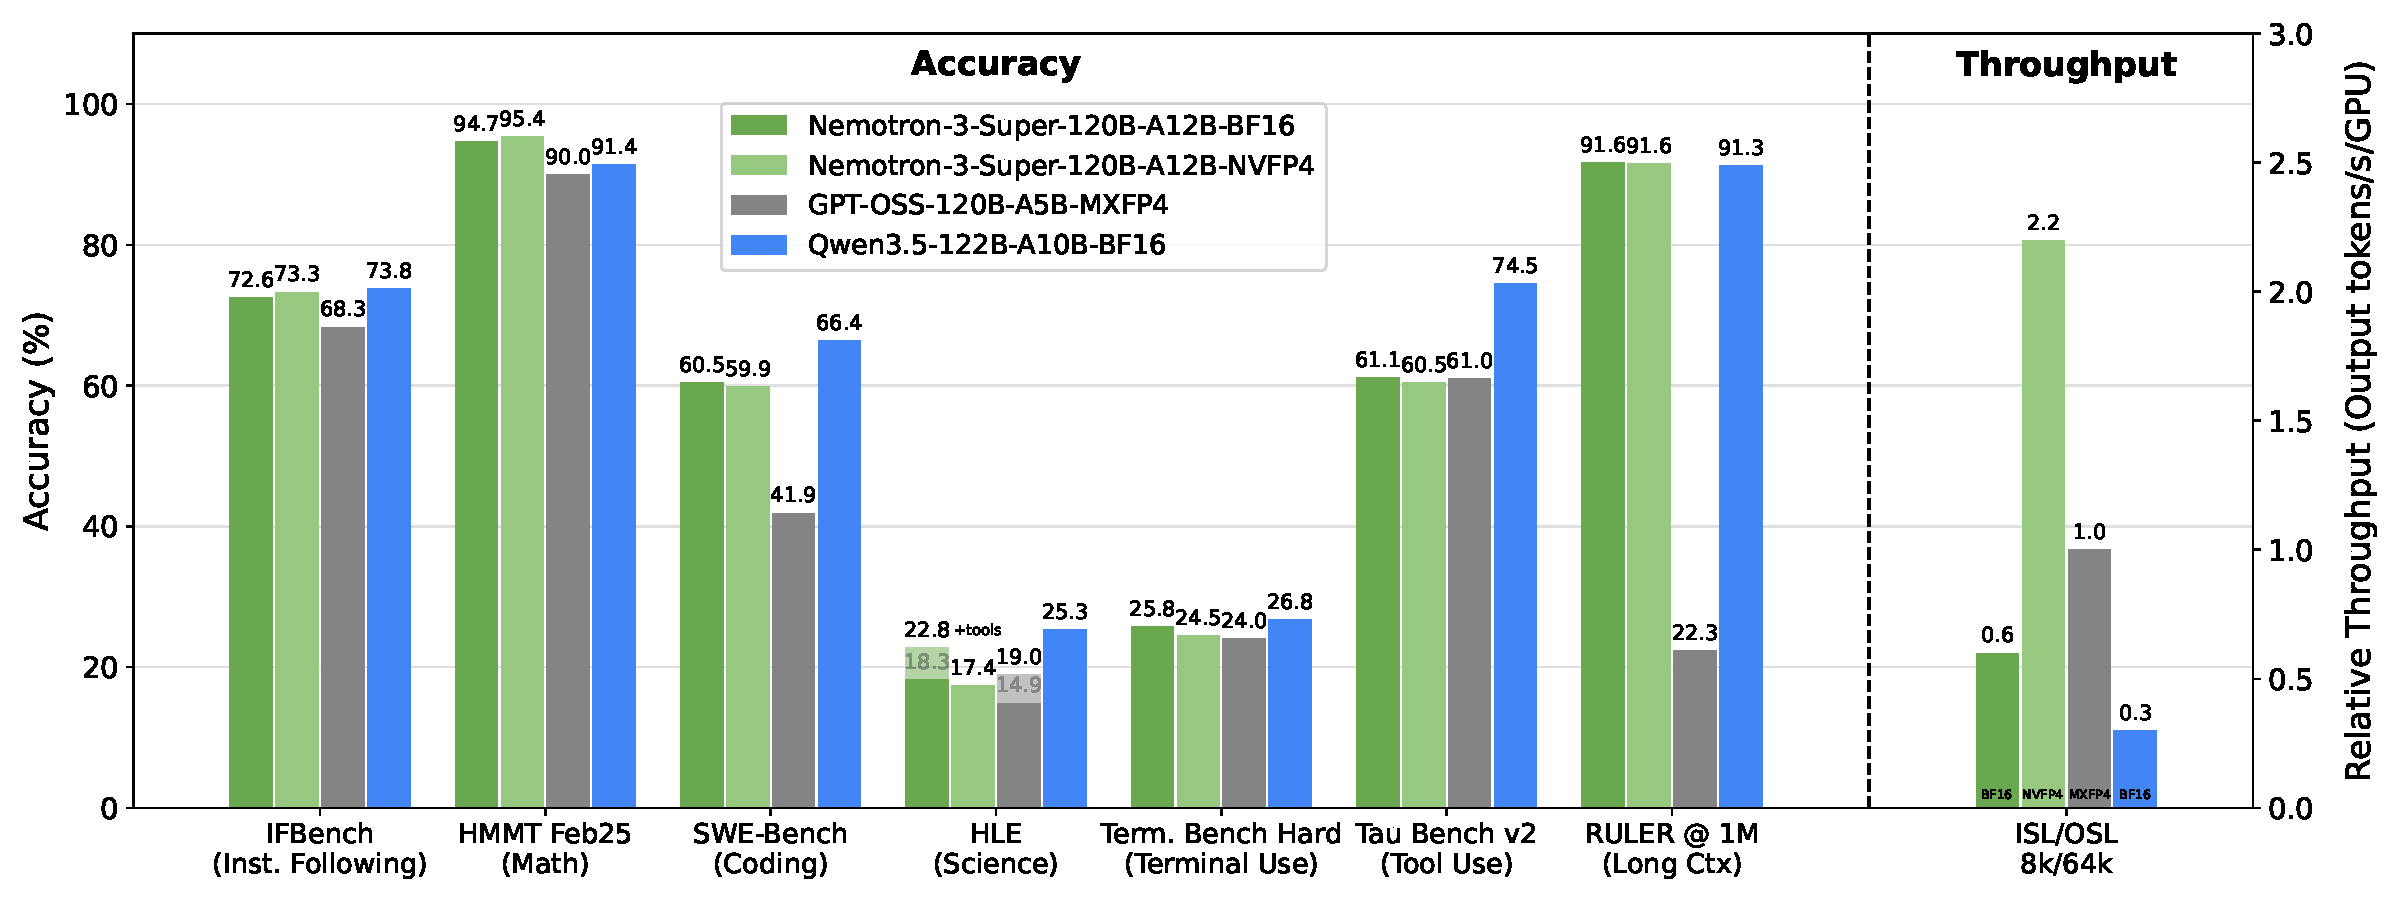
\includegraphics[width=\linewidth]{n3s-fig01-accuracy-throughput.pdf}
  \caption[Accuracy and throughput of Nemotron 3 Super against GPT-OSS-120B and Qwen3.5-122B]{Accuracy
  and throughput of \NS\ compared with GPT-OSS-120B and Qwen3.5-122B.
  Throughput is measured on B200 GPUs with 8k input and 64k output tokens.
  \source{NVIDIA (2026)~\cite{nvidia2026super}, Fig.~1}}
  \label{fig:headline}
\end{figure}

\begin{table}[htbp]
\centering
\small
\caption[Post-trained model comparison]{Post-trained \NS\ compared with
Qwen3.5-122B-A10B and GPT-OSS-120B on selected benchmarks
(from~\cite{nvidia2026super}, Table~5). Best value in each row in bold.}
\label{tab:main}
\begin{tabular}{@{}lccc@{}}
\toprule
\textbf{Benchmark} & \textbf{\NS} & \textbf{Qwen3.5-122B} & \textbf{GPT-OSS-120B} \\
\midrule
\multicolumn{4}{@{}l}{\emph{General knowledge and reasoning}} \\
MMLU-Pro & 83.73 & \textbf{86.70} & 81.00 \\
AIME25 (no tools) & 90.21 & 90.36 & \textbf{92.50} \\
HMMT Feb25 (no tools) & \textbf{93.67} & 91.40 & 90.00 \\
GPQA (no tools) & 79.23 & \textbf{86.60} & 80.10 \\
LiveCodeBench v5 & 81.19 & 78.93 & \textbf{88.00} \\
SciCode (subtask) & \textbf{42.05} & 42.00 & 39.00 \\
HLE (no tools) & 18.26 & \textbf{25.30} & 14.90 \\
\midrule
\multicolumn{4}{@{}l}{\emph{Agentic}} \\
Terminal Bench (hard subset) & 25.78 & \textbf{26.80} & 24.00 \\
Terminal Bench Core 2.0 & 31.00 & \textbf{37.50} & 18.70 \\
SWE-Bench (OpenHands) & 60.47 & \textbf{66.40} & 41.90 \\
TauBench V2 (average) & 61.15 & \textbf{74.53} & 61.00 \\
\midrule
\multicolumn{4}{@{}l}{\emph{Chat and instruction following}} \\
IFBench (prompt) & 72.56 & \textbf{73.77} & 68.32 \\
Arena-Hard-V2 & 73.88 & 75.15 & \textbf{90.26} \\
\midrule
\multicolumn{4}{@{}l}{\emph{Long context}} \\
AA-LCR & 58.31 & \textbf{66.90} & 51.00 \\
RULER 256k & \textbf{96.83} & 96.74 & 52.30 \\
RULER 512k & 95.22 & \textbf{95.95} & 46.70 \\
RULER 1M & \textbf{91.64} & 91.33 & 22.30 \\
\midrule
\multicolumn{4}{@{}l}{\emph{Multilingual}} \\
MMLU-ProX (average) & 79.36 & \textbf{85.06} & 76.59 \\
WMT24++ (en$\rightarrow$xx) & 86.67 & 87.84 & \textbf{88.89} \\
\bottomrule
\end{tabular}
\end{table}

Three observations can be made.

\textbf{Against GPT-OSS-120B.} \NS\ matches or beats GPT-OSS-120B on most of
the benchmarks listed. The lead is largest on agentic tasks---60.5 against
41.9 on SWE-Bench and 31.0 against 18.7 on Terminal Bench Core 2.0---which
reflects the emphasis on agentic data and RL environments during
post-training. GPT-OSS-120B remains ahead on a few benchmarks, notably
LiveCodeBench, AIME25 and Arena-Hard-V2.

\textbf{Against Qwen3.5-122B.} Qwen3.5-122B is the more accurate model on the
majority of rows: it leads on MMLU-Pro, GPQA, HLE, SWE-Bench, TauBench and
MMLU-ProX, in several cases by a clear margin. \NS\ is ahead on HMMT,
LiveCodeBench and RULER at 256k and 1M, and roughly level elsewhere. The
report itself describes the model as ``lagging behind Qwen-3.5-122B slightly''
on reasoning. The case for \NS\ over Qwen3.5 therefore rests on throughput
rather than on accuracy.

\textbf{Accuracy is ``comparable'', not uniformly better.} The fair summary is
that the hybrid model sits in the same accuracy class as the best open
Transformer MoE models of its size: ahead of one, somewhat behind the other.

\section{Long-Context Performance}

The clearest qualitative difference appears on RULER~\cite{hsieh2024ruler}, a
benchmark that measures how well a model actually uses a long context.
Figure~\ref{fig:ruler} plots the scores from Table~\ref{tab:main}. \NS\ loses
only about five points between 256k and one million tokens, finishing at
91.6. GPT-OSS-120B is already at 52.3 at 256k and falls to 22.3 at one million
tokens. Qwen3.5-122B, a Transformer, tracks \NS\ closely on this benchmark,
which shows that long-context \emph{accuracy} is not exclusive to hybrids;
what the hybrid changes is the \emph{cost} of serving such contexts.

\begin{figure}[htbp]
  \centering
  % RULER long-context accuracy, plotted from Table 5 of the Nemotron 3 Super report
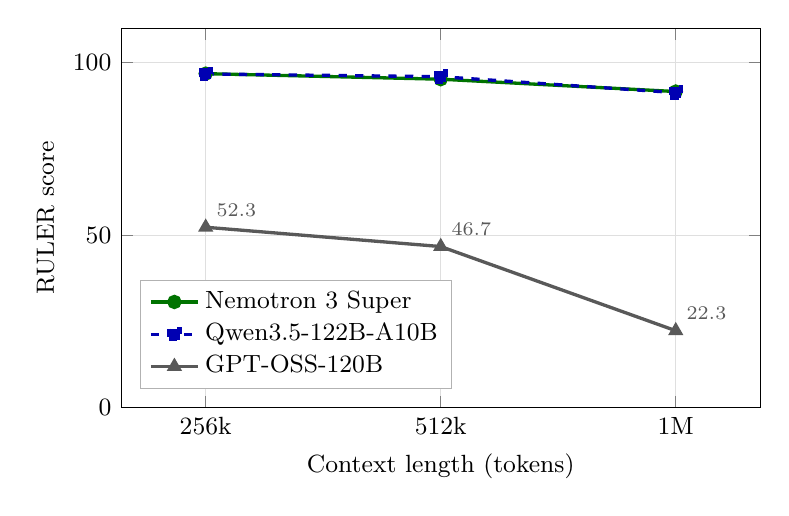
\begin{tikzpicture}
\begin{axis}[
  width=0.8\linewidth, height=6.4cm,
  symbolic x coords={256k,512k,1M}, xtick=data,
  xlabel={Context length (tokens)}, ylabel={RULER score},
  ymin=0, ymax=110, enlarge x limits=0.18,
  grid=major, grid style={gray!25},
  legend style={font=\small, at={(0.03,0.05)}, anchor=south west, draw=gray!60},
  legend cell align=left,
  tick label style={font=\small}, label style={font=\small},
  ]
\addplot[very thick, mark=*, green!45!black]
  coordinates {(256k,96.83) (512k,95.22) (1M,91.64)};
\addlegendentry{Nemotron 3 Super}
\addplot[very thick, mark=square*, blue!70!black, dashed]
  coordinates {(256k,96.74) (512k,95.95) (1M,91.33)};
\addlegendentry{Qwen3.5-122B-A10B}
\addplot[very thick, mark=triangle*, gray!70!black,
  nodes near coords, nodes near coords style={font=\scriptsize, anchor=south west}]
  coordinates {(256k,52.30) (512k,46.70) (1M,22.30)};
\addlegendentry{GPT-OSS-120B}
\end{axis}
\end{tikzpicture}

  \caption[RULER score against context length]{RULER score against context
  length for the three models (plotted by the author from the data
  in~\cite{nvidia2026super}, Table~5).}
  \label{fig:ruler}
\end{figure}

It is also notable that the score at one million tokens rose from 71.0 for the
base model (Table~\ref{tab:base}) to 91.6 after post-training, which included
long-context SFT data and a long-context RL environment.

\section{Inference Throughput}

Throughput is where the architecture pays off. On B200 GPUs, with 8k input
tokens and 64k output tokens---a setting typical of long reasoning or agentic
generation---\NS\ delivers up to 2.2$\times$ the throughput of GPT-OSS-120B
and up to 7.5$\times$ that of Qwen3.5-122B. Table~\ref{tab:throughput} lists
the relative values shown in Figure~\ref{fig:headline}.

\begin{table}[htbp]
\centering
\small
\caption[Relative inference throughput]{Relative inference throughput at 8k
input / 64k output tokens, normalised to GPT-OSS-120B (values read by the
author from~\cite{nvidia2026super}, Fig.~1)}
\label{tab:throughput}
\begin{tabular}{@{}llc@{}}
\toprule
\textbf{Model} & \textbf{Precision} & \textbf{Relative throughput} \\
\midrule
\NS\ 120B-A12B & NVFP4 & 2.2 \\
GPT-OSS-120B-A5B & MXFP4 & 1.0 \\
\NS\ 120B-A12B & BF16 & 0.6 \\
Qwen3.5-122B-A10B & BF16 & 0.3 \\
\bottomrule
\end{tabular}
\end{table}

Two details matter when reading these figures. First, the 2.2$\times$ result
belongs to the NVFP4 checkpoint; the unquantized BF16 checkpoint is slower
than the 4-bit GPT-OSS-120B. The headline speed is thus the product of the
architecture \emph{and} the quantization work of Chapter~\ref{ch:quant}, not
of the architecture alone. Second, at equal precision (BF16) \NS\ is about
twice as fast as Qwen3.5-122B even though it activates slightly more
parameters per token (12B against 10B). Here the difference does come from the
architecture: a long 64k-token generation is exactly the regime in which a
constant-size Mamba state beats a growing KV cache.

\section{Summary of Results}

\begin{itemize}
  \item The base model outperforms comparable public base models on nearly all
        benchmarks.
  \item The post-trained model matches or beats GPT-OSS-120B on most tasks and
        trails Qwen3.5-122B on several reasoning and agentic benchmarks.
  \item On RULER at one million tokens it scores 91.6, against 22.3 for
        GPT-OSS-120B.
  \item It runs up to 2.2$\times$ faster than GPT-OSS-120B and up to
        7.5$\times$ faster than Qwen3.5-122B.
  \item Quantization to NVFP4 retains a median of 99.8\% of BF16 accuracy, and
        MTP yields an average acceptance length of 3.45 tokens.
\end{itemize}

\chapter{Applications}
\label{ch:apps}

The design choices of \NS---a million-token context, high throughput on long
generations, and post-training focused on multi-step tool use---point to a
particular class of applications. The Nemotron~3 white paper positions Super
for collaborative agents and high-volume workloads such as IT ticket
automation~\cite{nvidia2025nemotron3}. The main application areas are outlined
below.

\section{Coding Agents}

A coding agent must read a repository, locate the cause of an issue, edit
several files and run the tests, often over dozens of steps. Each step adds
tool output to the context, so the context grows quickly and most of the work
is \emph{prefill}: processing a long input before a short action. This is the
workload for which the NVFP4 checkpoint was designed. \NS\ was trained for it
directly, with SFT data built from real GitHub issues and a dedicated
software-engineering RL stage, and it scores 60.5 on SWE-Bench with the
OpenHands harness (Table~\ref{tab:main}).

\section{Terminal and Multi-Step Task Automation}

Closely related are assistants that operate a command line: installing
software, inspecting logs, and chaining commands to complete an administrative
task. The model was trained on terminal-use data and is evaluated on Terminal
Bench. Long sessions benefit from the constant-size Mamba state, because the
cost of each new token does not climb as the session history accumulates in
the way it does for a model built only from attention layers.

\section{Tool-Using Agents and Customer Service}

Many business applications consist of a model calling external tools: querying
a database, searching the web, or invoking an API to check an order or change
a booking. \NS\ was trained with conversational and general-purpose
tool-calling data and with search and SQL datasets, and is evaluated on
TauBench (airline, retail and telecom customer-service scenarios), BrowseComp
(web search) and BIRD (text-to-SQL). High throughput matters here because such
systems serve many users at once and often run several model calls per
request.

\section{Long-Document Analysis}

With a context of one million tokens, entire contracts, sets of research
papers, financial reports or codebases can be given to the model at once,
instead of being cut into fragments and retrieved piecemeal. The RULER score
of 91.6 at one million tokens indicates that the model can actually locate and
use information at that range, rather than merely accept it as input.

\section{Reasoning with Controllable Effort}

The model supports three reasoning modes---off, regular and low-effort---which
can be combined with a reasoning budget set at inference time. An application
can thus spend long reasoning traces on hard problems and answer simple
requests quickly, trading accuracy against cost request by request.

\section{On-Premises and Customised Deployment}

Because the weights, the quantized checkpoints and much of the training data
are openly released, an organisation can run the model on its own hardware and
fine-tune it on its own data. This is important where data cannot leave the
organisation, for example in finance, healthcare or government. The FP8 and
NVFP4 checkpoints target the Hopper and Blackwell GPU generations
respectively, and the built-in MTP heads provide speculative decoding without
a separate draft model.

\chapter{Advantages and Limitations}
\label{ch:adv}

\section{Advantages}

\begin{enumerate}
  \item \textbf{Long context at low cost.} The model supports contexts of up
        to one million tokens. Because 40 of its 48 sequence-mixing layers are
        Mamba-2 blocks with a constant-size state, only 8 layers need a KV
        cache, and the cost of generating each new token grows far more slowly
        with context length than in a pure Transformer.
  \item \textbf{High throughput.} It runs up to 2.2$\times$ faster than
        GPT-OSS-120B and up to 7.5$\times$ faster than Qwen3.5-122B at
        comparable accuracy, in a long-generation setting.
  \item \textbf{Large capacity, small active size.} Only about 12 billion of
        the 120 billion parameters are used for any one token, so the compute
        per token is that of a much smaller model.
  \item \textbf{Hardware-aware MoE.} LatentMoE reduces the memory traffic and
        the routing traffic of each expert by a factor of four and uses the
        saving to run more experts, improving accuracy at about the same cost.
  \item \textbf{Built-in speculative decoding.} The shared-weight MTP heads act
        as an internal draft model, with an average of 3.45 tokens accepted
        per verification step and no separate draft model to deploy.
  \item \textbf{Efficient training and deployment precision.} Pretraining in
        4-bit NVFP4 was stable over 25 trillion tokens, and the 4-bit
        deployment checkpoint keeps a median of 99.8\% of full-precision
        accuracy.
  \item \textbf{Openness.} Base, post-trained and quantized checkpoints, much
        of the training data and the training recipe are released openly, so
        the work can be inspected, reproduced in part and built upon.
\end{enumerate}

\section{Limitations}

\begin{enumerate}
  \item \textbf{Memory footprint.} MoE reduces computation, not storage. All
        120 billion parameters must still be held in memory even though only a
        tenth are used per token, so the hardware requirements remain high.
  \item \textbf{Serving complexity.} Expert routing makes deployment more
        complicated than for a dense model: different tokens need different
        experts, and in multi-GPU serving tokens must be routed between
        devices. Combining Mamba, attention, MoE and MTP also means the serving
        software must support all four efficiently.
  \item \textbf{Sensitivity of the recurrent state.} Compressing the Mamba
        state causes rounding errors that build up over long outputs
        (Chapter~\ref{ch:quant}). The stochastic-rounding fix works, but it
        depends on hardware support that is specific to recent NVIDIA GPUs, and
        the underlying effect was observed rather than removed by training.
  \item \textbf{Hardware dependence of the headline speed.} The 2.2$\times$
        figure applies to the NVFP4 checkpoint on Blackwell GPUs. On hardware
        without native FP4 support the advantage is smaller.
  \item \textbf{Accuracy gap to the strongest competitor.} The model is still
        behind Qwen3.5-122B on several reasoning and agentic benchmarks,
        including GPQA, HLE, SWE-Bench and TauBench.
  \item \textbf{Lossy memory in most layers.} A Mamba state is a summary. Exact
        recall over long distances relies on just eight attention layers, and
        the published results do not include an ablation showing how accuracy
        changes with the number or placement of those layers at this scale.
  \item \textbf{Cost of training.} Pretraining on 25 trillion tokens followed
        by RL across 21 environments on thousands of GPUs is far beyond the
        reach of most organisations; the open release lowers the barrier to
        \emph{using} the model, not to reproducing it from scratch.
  \item \textbf{Vendor-reported results.} All figures in this report come from
        the developers' own technical reports. Independent evaluation on other
        hardware and other serving frameworks would be needed to confirm how
        general the advantages are.
\end{enumerate}

\section{Comparison at a Glance}

Table~\ref{tab:compare} places \NS\ beside a pure Transformer MoE model of the
same class.

\begin{table}[htbp]
\centering
\small
\caption{Hybrid Mamba--Transformer MoE compared with a pure Transformer MoE}
\label{tab:compare}
\begin{tabularx}{\linewidth}{@{}P{3.6cm}LL@{}}
\toprule
\textbf{Aspect} & \textbf{Pure Transformer MoE} & \textbf{\NS\ (hybrid)} \\
\midrule
Sequence mixing & Attention in every block & Mamba-2 in 40 blocks, attention in 8 \\
Generation memory & KV cache in every block & KV cache in 8 layers, fixed state elsewhere \\
Feed-forward part & Standard MoE at full width & LatentMoE in a 1024-dimensional latent space \\
Faster decoding & External draft model, if any & Built-in MTP heads \\
Deployment risk & Well understood & Recurrent state needs careful quantization \\
Tooling maturity & Very mature & Newer, fewer optimised runtimes \\
\bottomrule
\end{tabularx}
\end{table}

\chapter{Conclusion and Future Scope}
\label{ch:conclusion}

\section{Conclusion}

Pure Transformers become slow and memory-heavy on long inputs because
self-attention compares every pair of tokens and keeps a KV cache that grows
with the context. State-space models such as Mamba-2 avoid both costs by
carrying a constant-size state, but that state is a lossy summary. This
seminar studied \NS, a model that combines the two: 40 Mamba-2 blocks carry
most of the sequence processing, 8 attention layers act as global anchors for
exact long-range retrieval, and 40 LatentMoE layers provide capacity.

Three further ideas complete the design. LatentMoE moves the experts into a
1024-dimensional latent space, which cuts memory and routing traffic fourfold
and pays for more experts, so that 120 billion parameters exist while only
about 12 billion are active for each token. Shared-weight multi-token
prediction heads give the model its own draft mechanism for speculative
decoding. Pretraining in 4-bit NVFP4 shows that low-precision training is
stable even over 25 trillion tokens.

The published results show a model in the same accuracy class as the best
open Transformer models of its size---ahead of GPT-OSS-120B on most tasks and
somewhat behind Qwen3.5-122B---while running up to 2.2$\times$ and
7.5$\times$ faster than them and holding a RULER score of 91.6 at one million
tokens. The study also showed that the hybrid approach is not free: it brings
new engineering problems, of which the accumulation of rounding error in the
Mamba state is the clearest example.

The broader lesson is that attention does not have to be everywhere. Used
sparingly and placed carefully, a handful of attention layers appear to be
enough, and the rest of the network can be built from cheaper components.
\NS\ is strong evidence that the next generation of efficient large-scale
models will be hybrids designed together with the hardware they run on, rather
than pure Transformers.

\section{Future Scope}

Several directions follow from this study.
\begin{itemize}
  \item \textbf{Larger hybrids.} The Nemotron~3 family includes a larger
        \emph{Ultra} model~\cite{nvidia2025nemotron3}; it will show whether the
        same layout continues to scale.
  \item \textbf{Placement and number of attention layers.} The ratio of about
        8--9\% attention comes from experiments on small models. A systematic
        study at large scale, or a learned placement, could improve the
        trade-off further.
  \item \textbf{Quantization-robust state-space layers.} The Mamba state
        currently needs a training-free fix at deployment. Training methods
        that make the recurrence itself robust to low-precision storage would
        remove a source of fragility and might allow the state to be stored in
        fewer bits.
  \item \textbf{Lower-precision training everywhere.} Several layer types are
        still trained in BF16. Extending 4-bit training to them, and
        understanding the growth of zero-valued gradients, would reduce
        training cost further.
  \item \textbf{Independent benchmarking.} Reproducing the throughput results
        on other accelerators and serving stacks would clarify how much of the
        advantage is architectural and how much is specific to one hardware
        platform.
  \item \textbf{Other modalities.} Linear-time sequence layers are attractive
        wherever sequences are very long, such as audio, video and genomic
        data; hybrid backbones could be extended to multimodal models.
  \item \textbf{Smaller footprints.} Techniques for loading experts on demand
        or pruning rarely used experts could reduce the memory needed to hold
        all 120 billion parameters and bring such models to smaller
        deployments.
\end{itemize}


% ================================================================ references
\clearpage
\phantomsection\addcontentsline{toc}{chapter}{References}
\renewcommand{\bibname}{References}
\begingroup
\singlespacing
\bibliographystyle{IEEEtran}
\bibliography{refs}
\endgroup

\end{document}
